\documentclass[a4paper,12pt]{article}

\documentclass[a4paper,12pt]{article}

%%% Работа с русским языком
\usepackage{cmap}					% поиск в PDF
\usepackage{mathtext} 				% русские буквы в формулах
\usepackage[T2A]{fontenc}			% кодировка
\usepackage[utf8]{inputenc}			% кодировка исходного текста
\usepackage[english,russian]{babel}	% локализация и переносы
\usepackage{indentfirst}            % красная строка в первом абзаце
\frenchspacing                      % равные пробелы между словами и предложениями

%%% Дополнительная работа с математикой
\usepackage{amsmath,amsfonts,amssymb,amsthm,mathtools} % пакеты AMS
\usepackage{icomma}                                    % "Умная" запятая

%%% Свои символы и команды для математики, обозначений
\usepackage{centernot} % центрированное зачеркивание символа
\usepackage{stmaryrd}  % некоторые спецсимволы

\renewcommand{\phi}{\ensuremath{\varphi}}
\renewcommand{\kappa}{\ensuremath{\varkappa}}
\renewcommand{\le}{\ensuremath{\leqslant}}
\renewcommand{\leq}{\ensuremath{\leqslant}}
\renewcommand{\ge}{\ensuremath{\geqslant}}
\renewcommand{\geq}{\ensuremath{\geqslant}}
\renewcommand{\emptyset}{\ensuremath{\varnothing}}

\DeclareMathOperator{\sgn}{sgn}
\DeclareMathOperator{\Arg}{Arg}
\DeclareMathOperator{\Ln}{Ln}
\DeclareMathOperator{\re}{Re}
\DeclareMathOperator{\im}{Im}
\DeclareMathOperator{\dlim}{\underline{lim}}

\newcommand{\N}{\mathbb{N}}
\newcommand{\Z}{\mathbb{Z}}
\newcommand{\Q}{\mathbb{Q}}
\newcommand{\R}{\mathbb{R}}
\newcommand{\Cm}{\mathbb{C}}
\newcommand{\F}{\mathbb{F}}
\newcommand{\id}{\mathrm{id}}
\newcommand{\goth}{\mathfrak}
\newcommand{\eps}{\varepsilon}
\newcommand{\veps}{\epsilon}
\newcommand{\liml}{\lim\limits}

\newcommand{\System}[1]{
	\left\{\begin{aligned}#1\end{aligned}\right.
}
\newcommand{\Root}[2]{
	\left\{\!\sqrt[#1]{#2}\right\}
}

\renewcommand\labelitemi{$\triangleright$}

\let\bs\backslash
\let\lra\Leftrightarrow
\let\ra\rightarrow
\let\rra\rightrightarrows
\let\Ra\Rightarrow
\let\la\Leftarrow
\let\emb\hookrightarrow

\newcommand{\dse}{\displaystyle}

%%% Перенос знаков в формулах (по Львовскому)
\newcommand*{\hm}[1]{#1\nobreak\discretionary{}{\hbox{$\mathsurround=0pt #1$}}{}}

%%% Работа с картинками
\usepackage{graphicx}    % Для вставки рисунков
\setlength\fboxsep{3pt}  % Отступ рамки \fbox{} от рисунка
\setlength\fboxrule{1pt} % Толщина линий рамки \fbox{}
\usepackage{wrapfig}     % Обтекание рисунков текстом

%%% Работа с таблицами
\usepackage{array,tabularx,tabulary,booktabs} % Дополнительная работа с таблицами
\usepackage{longtable}                        % Длинные таблицы
\usepackage{multirow}                         % Слияние строк в таблице

%%% Теоремы
\theoremstyle{plain}
\newtheorem{theorem}{Теорема}[section]
\newtheorem{lemma}{Лемма}[section]
\newtheorem{proposition}{Утверждение}[section]
\newtheorem*{exercise}{Упражнение}

\theoremstyle{definition}
\newtheorem{definition}{Определение}[section]
\newtheorem*{adefinition}{Определение(не материал лектора)}
\newtheorem*{corollary}{Следствие}
\newtheorem*{addition}{Дополнение}
\newtheorem*{note}{Замечание}
\newtheorem*{anote}{Замечание автора}
\newtheorem*{reminder}{Напоминание}
\newtheorem*{example}{Пример}
\newtheorem*{examples}{Примеры}

\theoremstyle{remark}
\newtheorem*{solution}{Решение}

%%% Оформление страницы
\usepackage{extsizes}     % Возможность сделать 14-й шрифт
\usepackage{geometry}     % Простой способ задавать поля
\usepackage{setspace}     % Интерлиньяж
\usepackage{enumitem}     % Настройка окружений itemize и enumerate
\setlist{leftmargin=25pt} % Отступы в itemize и enumerate

\geometry{top=25mm}    % Поля сверху страницы
\geometry{bottom=30mm} % Поля снизу страницы
\geometry{left=20mm}   % Поля слева страницы
\geometry{right=20mm}  % Поля справа страницы

\setlength\parindent{15pt}        % Устанавливает длину красной строки 15pt
\linespread{1.3}                  % Коэффициент межстрочного интервала
%\setlength{\parskip}{0.5em}      % Вертикальный интервал между абзацами
%\setcounter{secnumdepth}{0}      % Отключение нумерации разделов
%\setcounter{section}{-1}         % Нумерация секций с нуля
\usepackage{multicol}			  % Для текста в нескольких колонках
\usepackage{soulutf8}             % Модификаторы начертания

%%% Шаблонная информация для титульного листа
\newcommand{\CourseName}{Основы комбинаторики и теории чисел}
\newcommand{\FullCourseNameFirstPart}{\so{ОСНОВЫ КОМБИНАТОРИКИ И ТЕОРИИ ЧИСЕЛ}}
\newcommand{\SemesterNumber}{I}
\newcommand{\LecturerInitials}{Райгородский Андрей Михайлович, Мусатов Даниил Владимирович}
\newcommand{\CourseDate}{осень 2021}
\newcommand{\GithubLink}{https://github.com/MIPT-Group/Lectures_Tex_Club}

%%% Колонтитулы
\usepackage{titleps}
\newpagestyle{main}{
	\setheadrule{0.4pt}
	\sethead{\CourseName}{}{\hyperlink{intro}{\;Назад к содержанию}}
	\setfootrule{0.4pt}                       
	\setfoot{ФПМИ МФТИ, \CourseDate}{}{\thepage} 
}
\pagestyle{main}  

%%% Нумерация уравнений
\makeatletter
\def\eqref{\@ifstar\@eqref\@@eqref}
\def\@eqref#1{\textup{\tagform@{\ref*{#1}}}}
\def\@@eqref#1{\textup{\tagform@{\ref{#1}}}}
\makeatother                      % \eqref* без гиперссылки
\numberwithin{equation}{section}  % Нумерация вида (номер_секции).(номер_уравнения)
\mathtoolsset{showonlyrefs=false} % Номера только у формул с \eqref{} в тексте.

%%% Гиперссылки
\usepackage{hyperref}
\usepackage[usenames,dvipsnames,svgnames,table,rgb]{xcolor}
\hypersetup{
	unicode=true,            % русские буквы в раздела PDF
	colorlinks=true,       	 % Цветные ссылки вместо ссылок в рамках
	linkcolor=black!15!blue, % Внутренние ссылки
	citecolor=green,         % Ссылки на библиографию
	filecolor=magenta,       % Ссылки на файлы
	urlcolor=NavyBlue,       % Ссылки на URL
}

%%% Графика
\usepackage{tikz}        % Графический пакет tikz
\usepackage{tikz-cd}     % Коммутативные диаграммы
\usepackage{tkz-euclide} % Геометрия
\usepackage{stackengine} % Многострочные тексты в картинках
\usetikzlibrary{angles, babel, quotes}

\newcommand{\CourseName}{ТФКП} %  Используется в преамбуле для создания названия предмета в верхнем контитуле   
\newcommand{\CourseDate}{Осень 2020}           %  Используется в преамбуле для создания даты в нижнем контитуле

%\includeonly{lectures/lect05,lectures/lect06}  % Чтобы скомпилировать только часть лекций

\begin{document}
    \begin{titlepage}
	\clearpage\thispagestyle{empty}
	\centering
	
	\textbf{Московский физико-технический институт \\ Физтех-школа прикладной математики и информатики}
	\vspace{33ex}
	
	{\textbf{\FullCourseNameFirstPart}}
	
	\SemesterNumber\ СЕМЕСТР  
	\vspace{1ex}
	
	Лектор: \textit{\LecturerInitials}
	
	
\includegraphics[width=0.4\textwidth]{images/logo_ltc.png}

	\begin{flushright}
		\noindent
		Автор: \href{\VKLink}{\textit{\AuthorInitials}}
		\\
		\href{\GithubLink}{\textit{Проект на Github}}
	\end{flushright}
	
	\vfill
	\CourseDate
	\pagebreak
\end{titlepage}

    \hypertarget{intro}{}
    \tableofcontents
    \newpage
    \begin{flushright}
    \textit{Лекция 1 (от 07.09)}
\end{flushright}
\section{$\S 1.$ Комплексные числа}
\Def
Пусть $z = \left( x;y \right) \in \RR^2$. Пусть определены операции:
\begin{enumerate}
    \item \textbf{Сложение:} $z_1 + z_2 = \left( x_1+x_2; y_1+y_2 \right)$
    \item \textbf{Умножение на действительное число:} $\lambda z = \left(\lambda
        x, \lambda y \right)$
    \item \textbf{Расстояние:} $\rho(z_1, z_2) = \left| \left| z_1 - z_2 \right|
    \right| = \sqrt{\left( x_1 - x_2 \right)^2 + (y_1 - y_2)^2}$
\end{enumerate}
Добавим операцию
умножения друг на друга:
\begin{equation}
  z_1 \cdot z_2 = \left( x_1 \cdot x_2 - y_1 \cdot y_2; x_1 \cdot y_2 + x_2 \cdot y_1 \right)
\end{equation}
Будем называть это \textbf{комплексными числами} $\CC$.

Пусть $1 \sim (1; 0)$~--- \textbf{единица}, $i \sim (0;1)$~--- \textbf{мнимая
  единица}.

Тогда $z = 1 \cdot x + i \cdot y \Leftrightarrow z = x + iy$~---
\textbf{алгебраическая запись}.
\section{$\S 2.$ Последовательность. Предел. Ряды. Функции. Расширенная
  комплексная плоскость}

    \begin{flushright}
    \textit{Лекция 2 (от 08.09)}
\end{flushright}
\section{$\S 3.$ Дифференцирование}
\section{$\S 4.$ Регулярные и гармонические функции}

    \begin{flushright}
    \textit{Лекция 3 (от 14.09)}
\end{flushright}
\section{$\S 5.$ Теорема об обратной функции}
\theorem
Пусть $f: G \mapsto H \subseteq \CC$, $g: H \mapsto \CC$ регулярны.
Тогда $\zeta(z) = g(f(z)): G \mapsto \CC$ также регулярна, причем
\begin{equation}\label{(5.1)}
    \zeta'(z) = g'(f(z))f'(z) \forall z \in G
\end{equation}
\pr
\begin{align*}
  & z_0 \in G, \ w_0 = f(z_0) \in H
\end{align*}
Из дифференцируемости
\begin{align*}
  & \Delta f = f(z_0)\Delta z + o(\Delta z), \ \Delta g = g'(w_0) \Delta w + 0(\Delta w)
\end{align*}
Пусть $\Delta w = \Delta f$, тогда
\begin{align*}
  & \frac{\Delta \zeta}{\Delta z} = g'(w_0) \frac{\Delta f}{\Delta z} + \frac{o(\Delta f)}{\Delta f} \cdot \frac{\Delta f}{\Delta z} \us{\Delta z \to 0}{\to} g'(w_0)f'(z_0) + 0
\end{align*}
\theorem (об обратной функции)
Пусть $f: G \mapsto \CC$ регулярна и непрерывно дифференцируема на $G$. Пусть
$z_0 \in G$, $w_0 = f(z_0)$, $f'(z_0) \neq 0$. Тогда $\exists B_\delta(z_0),
B_\varepsilon(w_0)$, такие, что:
\begin{enumerate}
    \item $\forall z \in B_\delta(z_0) \ f'(z) \neq 0$;
    \item $\forall \hat{w} \in B_\varepsilon(w_0)$ уравнение $\hat{w} = f(z)$
    имеет в $B_\delta(z_0)$ единственное решение $\hat{z}$, т.~е. на
    $B_\varepsilon(w_0)$ определена обратная функция $g: B_\varepsilon(w_0)
    \mapsto B_\delta(z_0)$, т.~е. $\forall w \in B_\delta(w_0) \hookrightarrow
    f(g(w)) = w$;
    \item $g$ регулярна на $B_\varepsilon(w_0)$, причем
    \begin{align*}
      & \forall w \in B_\varepsilon(w_0) \hookrightarrow g'(w) = \frac{1}{f'(g(w))}
    \end{align*}
\end{enumerate}
\pr
Пусть $f(z) = u(x,y) +iv(x,y)$. Имеем отображение $\RR^2 \mapsto \RR^2$. В силу
непрерывной дифференцируемости этих двух функций запишем якобиан и преобразуем
согласно УКР:
\begin{align*}
  & J(x,y) = \left| \begin{matrix}
          u_x & u_y \\
          v_x & v_y
      \end{matrix} \right| = \left| \begin{matrix}
          u_x & -v_x \\
          v_x & u_x
      \end{matrix} \right| = (u_x)^2+(v_x)^2 = \left| f'(z) \right|^2
\end{align*}
\begin{align*}
  & J(x_0,y_0) \neq 0
\end{align*}
\theorem (Бесов, $\S 12.1$, $1$)
Для такого отображения, как в теореме $5.2$, $\exists B_\delta(z_0): \ \forall z
\in B_\delta(z_0) \ f'(z) \neq 0 $, а также $\exists B_\varepsilon(z_0)$, где
существует обратное отображение
\begin{align*}
  & \left\{ \begin{matrix}
          x = x(u,v) \\
          y = y(u,v)
      \end{matrix} \right.: B_\varepsilon(w_0) \mapsto B_\delta(z_0)
\end{align*}
причем непрерывно дифференцируемое.
\pr
\begin{align*}
  & g(w) = z = x(u,v) + iy(u,v): B_\varepsilon(w_0) \mapsto B _\delta(z_0)
\end{align*}
Докажем, что
\begin{align*}
  &\forall w \in B_\varepsilon(w_0) \ \exists g'(w)
\end{align*}
Действительно,
\begin{align*}
  & \forall \hat{w} \in B_\varepsilon(w_0) \ \exists \hat{z} \in B_\delta(z_0): \ f(\hat{z}) = \hat{w} \Leftrightarrow g(\hat{w}) = \hat{z}
\end{align*}
\begin{align*}
  & \forall \left\{ w_k \right\}_{k=1}^\infty \subseteq B_\varepsilon(w_0): \ \forall k \ w_k \neq \hat{w}, \ w_k \us{k \to \infty}{\to} \hat{w} \ \exists z_k = g(w_k): \ \forall k \ f(z_k) = w_k; \ z_k \us{k \to \infty}{\to} z
\end{align*}
\begin{align*}
  & \frac{g(w_k) - g(\hat{w})}{w_k - \hat{w}} = \frac{z_k - \hat{z}}{w_k - \hat{w}} = \frac{1}{\dst \frac{f(z_k) - f(\hat{z})}{z_k - \hat{z}}} \us{k \to \infty}{\to} \frac{1}{f'(\hat{z})}
\end{align*}
\corollary
Пусть $f: G \mapsto \CC$ \textbf{однолистна} (взаимно однозначна) на $G$,
регулярна на этой области и имеет непрерывную производную. Пусть $\forall z \in
G \ f'(z) \neq 0$. Тогда обратное отображение $g: G^* \mapsto \CC$, причем
$g(G^*) = G$, регулярно на $G^*$.
\pr
Докажем, что $G^*$~--- область. Видим, что $\forall w_0 \in G^* \ \exists z_0
\in G: \ f(z_0) = w_0$. По условию, $f'(z) \neq 0$; тогда по теореме $2$ $\S 5$
$\exists \varepsilon > 0: \ B_\varepsilon(w_0) \subseteq G^*$.
\\
Докажем регулярность.
\begin{align*}
  & w_1, w_2 \in G \Rightarrow \exists z_1, z_2 \in G: \ f(z_k) = w_k
\end{align*}
Заметим, что $\exists \gamma_{z_1z_2} \subseteq G$; тогда $\gamma_{w_1w_2}^* =
\gamma^* = f(\gamma_{z_1z_2}) \subseteq G^*$.
В силу дифференцируемости $g$ в $B_\varepsilon(w_0)$ $g$ будет регулярна на
$G^*$.
\Example
$w = z^n, \ n \geq 2, \ n \in \NN$.
\\
Уравнение $z^n = w_0$ имеет решения:
\begin{align*}
  & z \in \left\{ \sqrt[n]{w_0} \right\} = \left\{ \sqrt[n]{\left| w_0 \right|} \exp \left( \dst \frac{i}{n}\left( \argt w_0 + 2 \pi k \right) \right) \mid k \in \left\{0, \dots, n-1 \right\} \right\}
\end{align*}
\Def
Пусть $\forall z \in G$ поставлено в соответствие некоторое множество $F(z)
\subseteq \CC$. Тогда говорят, что $F$~--- \textbf{многозначная функция}.
\\
Для нашего примера $F(w) = \left\{ \sqrt[n]{w} \right\}, \ w \in \CC$.
\Def
Пусть $F: G \mapsto 2^{\CC}$, $f: G \mapsto \CC$, $\forall z \in G \ f(z)\in
F(z)$. Тогда $f$~--- \textbf{ветвь многозначной функции} $F$.
\Example
\begin{align*}
  & z_1^n = z_2^n \Leftrightarrow \left| z_1 \right|^n \exp \left( in\varphi_1 \right) = \left| z_2 \right|^n \exp \left( in\varphi_2 \right) \Leftrightarrow \left| z_1 \right| = \left|z_2\right|, \ n\left( \varphi_1 - \varphi_2 \right) = 2 \pi k, \ k \in \ZZ
\end{align*}
Рассмотрим область
\begin{align*}
  & G_{\alpha, \beta} = \left\{ z \mid z = re^{i \varphi}, \ r>0, \ \varphi \in \left( \alpha, \beta \right) \right\}
\end{align*}
Если $0 < n(\beta - \alpha) \leq 2 \pi$, то $w = z^n$ будет однолистной. По
следствию $1$ существует обратная $g(w)$, причем регулярная. Эта функция
строится для случая $\alpha = -\frac{\pi}{2}$, $\beta = \frac{\pi}{2}$ так:
\begin{align*}
  & g: G_{-\frac{\pi}{2}, \frac{\pi}{2}} \mapsto G_{-\frac{n\pi}{2}, \frac{n\pi}{2}} \subseteq \CC \setminus (-\infty; 0]; \ l_{\varphi_0} = \left\{ z \mid z = re^{\i \varphi_0}, \ r > 0 \right\}, \ l_{\varphi_0} \mapsto l_{n \varphi_0}
\end{align*}
В явном виде функция будет иметь вид
\begin{align*}
  & g(w) = \sqrt[n]{\left| w \right|}\exp\left( \frac{i}{n} \argm w \right)
\end{align*}
Это \textbf{главная ветвь многозначной функции $\sets{\sqrt[n]{z}}$}.
\Example
$w = e^z$, $w'(z) \neq 0$.
\\
Отыщем область однолистности. Если $z_1 \neq z_2$, а $e^{z_1} = e^{z_2}$, то
$x_1 = x_2$, $y_1 - y_2 = 2 \pi k, \ k \in \ZZ$. Пусть $G_0 = \left\{ z \mid
    \Img z \in (-i\pi, i \pi) \right\}$. Тогда по следствию $5.3.1$ существует
обратная $g: \CC \setminus (-\infty; 0] \mapsto G_0$, причем регулярная. Эта
функция строится так:
\begin{align*}
  & e^z = w_0; \ e^x = \left| w_0 \right|, \ y = \alpha + 2 \pi k
\end{align*}
Имеем логарифм:
\begin{align*}
  & \Ln z = \ln \left| w \right| + i \Arg w
\end{align*}
Функция в явном виде имеет вид:
\begin{align*}
  & g = \ln \left| w \right| + i \argm w
\end{align*}
Это \textbf{главная ветвь многозначной функции $\Ln z$}.
\Example
Производная главной ветви логарифма
\begin{align*}
  & g'(w) = \frac{1}{w}
\end{align*}
а корня
\begin{align*}
  & g'(w) = \frac{1}{n(g(w))^{n-1}}
\end{align*}
\section{$\S 6.$ Интегрирование}
Задание $z(t) = x(t) + iy(t)$, $t \in [t_0;t_1]$, $x, y \in C[t_0, t_1]$
называется \textbf{параметрическим заданием кривой}.
\\
Если $t = \psi(\tau)$, $\tau \in [\tau_0; \tau_1]$ и функция непрерывно моотонно
возрастает, то это называется \textbf{эквивалентными параметризациями}.
\\
Множество эквивалентных параметризаций называется \textbf{кривой}.
\\
Кривая называется \textbf{жордановой (простой)}, если $\tau_1 \neq \tau_2
\Rightarrow z(\tau_1) \neq z(\tau_2)$, \textbf{гладкой}, если она непрерывно
дифференцируема, и \textbf{замкнутой}, если $z(\tau_0) = z(\tau_1)$
(\textbf{начальная} и \textbf{конечная} точки совпадают).
\\
Наконец, кривая называется \textbf{замкнутой жордановой}, если совпадение
разрешено только на концах.
\theorem (Жордана)
Всякая замкнутая ломаная жорданова кривая разбивает комплексную плоскость на
ограниченную (не содержащую $\infty$) и неограниченную, причем в ограниченной
облсти существует триангуляция с ориентацией: можно построить непересекающиеся
отрезки, разбивающие плоскость на треугольники, а на треугольниках задано
направление обхода, что совпадает на границе области с направлением обхода
кривой.
\pr (схема)
\\
Доказывать можем по индукции числа вершин ломаной.
\\
База: $n = 3$, очевидно, есть и область, и триангуляция.
\\
Шаг: допустим, есть вершина $A$ с максимальной действительной частью. Рассмотрим
соседние вершины: предшествующую $B$ и последующую $C$. Если ни в треугольнике,
ни на его границах нет вершин ломаной, то добавляем отрезок $BC$ и ориентацию
ему в обе стороны. Иначе, если внутри треугольника или на стороне $BC$ есть еще
одна вершина (пусть $D$, ближайшая к точке $A$), то включим в триангуляцию
отрезок $AD$.
    \begin{flushright}
    \textit{Лекция 4 (от 15.09)}
\end{flushright}

\textbf{Кривая} $\gamma$~--- класс эквивалентных параметризаций $z(t) = x(t) +
iy(t), \ t \in \left[ t_0; t_1 \right]$
\\
\textbf{Параметризации эквивалентны}, если существует монотонная возрастающая
функция $\psi(\tau) = t$, сохраняющая направление.
\\
\textbf{Гладкая кривая (ГК)}~--- такая кривая $\gamma$, что существует параметризация
$z(t) = x(t) + iy(t)$, $x \in C^1 \left( \left[ t_0; t_1 \right] \right)$, $y
\in C^1 \left( \left[ t_0; t_1 \right] \right)$, $\forall t \in \left[ t_0; t_1
\right] \ z'(t) \neq 0$.
\\
\textbf{Замкнутая ГК (ЗГК)}~--- такая ГК, что $z(t_0) = z(t_1)$, $z'(t_0+0) =
z'(t_1-0)$.
\\
\textbf{Кусочно гладкая кривая (КГК)}~--- такая непрерывная кривая $\gamma$, что
$\exists t_0 = \theta_0 < \theta_1 < \dots < \theta_{n-1} < \theta_n = t_1$, что
$\forall k \ \gamma_k: \ z(t), \ t \in [\theta_{k-1}, \theta_k]$ есть ГК.
\\
\textbf{Разбиение} отрезка $\left[ t_0, t_1 \right]$: $\lambda = \{t_0 = \tau_0
< \tau_1 < \dots < \tau_{m_\lambda} = t_1\}$.
\\
\textbf{Мелкость (диаметр)} разбиения $\lambda$ $\left| \lambda \right| = \dst
\max_{k \{1, \dots, m_\lambda\}}\left| \tau_k - \tau_{k-1} \right|$.
\Def Пусть $f: \gamma \mapsto \CC$ непрерывна на КГК $\gamma$. Пусть
$\lambda$~--- разбиение $\left[ t_0, t_1 \right]$ для $\gamma: \ z(t)$~---
кусочно гладкой. Пусть $z(t_k) = z_k, \ k \in \{0, \dots, m_\lambda\}$, $\zeta_k
\in$
\[\sigma(\lambda) = \sum_{k = 1}^{m_{\lambda}} f(\zeta_k) \Delta z_k\]
$\Delta z_k = z_k - z_{k-1}$~--- \textbf{интегральная сумма};
\\
если $\exists \lim
\sigma(\lambda) \forall \zeta_k, \ \left| \lambda \right| \to 0$, то этот предел
называется \textbf{интегралом Римана от $f$ по $\gamma$} и записывается как
\begin{equation} \label{(6.1)}
  \int_{\gamma}f(z) dz
\end{equation}
\theorem
Если условия определения интеграла выполняются, то он существует и справедливо:
\begin{equation} \label{(6.2)}
    \int_{\gamma}f(z)dz = \int_{\gamma}\left( u dx - v dy \right) + i \int_\gamma \left( v dx + u dy \right)
    \end{equation}
\pr
\begin{align*}
  & \sigma(\lambda) = \sum_{k = 1}^{m_\lambda}\left( u(\xi_k, \eta_k) + iv(\xi_k, eta_k) \right)\left( \Delta x_k + i \Delta y_k \right) = \sum_{k = 1}^{m_\lambda}\left( u(\xi_k, \eta_k) \Delta x_k - v(\xi_k, \eta_k) \Delta y_k\right) + \\
  & + \left( v(\xi_k, \eta_k) \Delta x_k + u(x_k, y_k) \Delta y_k\right) = \sigma_1(\lambda) + \sigma_2(\lambda) \to \int_{\gamma}\left( u dx - v dy \right) + i \int_\gamma \left( v dx + u dy \right)
\end{align*}
\corollary
Если условия определения интеграла выполняются, то верно:
\begin{equation} \label{(6.3)}
  \int_\gamma f(z) dz = \int_{t_0}^{t_1}f(z(t))z'(t)dt
\end{equation}
\begin{equation} \label{(6.4)}
  \gamma: z(t), \ \int_{t_0}^{t_1}\left( P(t) + iQ(t) \right) dt = \int_{t_0}^{t_1}P(t)dt + i \int_{t_0}^{t_1}Q(t)dt
\end{equation}
\pr
Из (\ref{(6.2)}) и свойств криволинейных интегралов II рода
\begin{align*}
  &\int_{\gamma}P(x,y) dx + Q(x,y)dy = \int_{t_0}^{t_1} \left( P(x(t), y(t)x'(t) + Q(x(t), y(t))y'(t) \right) dt
\end{align*}
\underline{\textbf{Общие свойства интеграла}}
\begin{enumerate}
    \item Линейность:
    \begin{align*}
      &\int_{\gamma}\left(\lambda f(z) + \mu g(z)\right) dz = \lambda\int_{\gamma}f(z) dz + \mu \int_\gamma g(z) dz
    \end{align*}
    \item Аддитивность вдоль кривой: если $\gamma = \gamma_1 \cup \gamma_2$
    (общая точка~--- только конец), то
    \begin{align*}
      &\int_{\gamma}f(z) dz = \int_{\gamma_1}f(z) dz \int_{\gamma_2} f(z) dz
    \end{align*}
    \item Изменение знака при смене направления: если $\gamma^{-1}$~---
    кривая, совпадающая во всех точках с $\gamma$, но противоположно
    направленная, то
    \begin{align*}
      &\int_{\gamma^{-1}}f(z) dz = - \int_{\gamma}f(z) dz
    \end{align*}
    \item Инвариантность относительно замены параметра.
    \item \prop Выполняется неравенство:
    \begin{equation} \label{(6.5)}
      \left| \int_\gamma f(z) dz \right| \leq \int_{\gamma}\left| f(z) \right| \cdot \left| dt \right| = \int_{t_0}^{t_1} \left| f(z(t)) \right| \sqrt{(x'(t))^2 + (y'(t))^2}dt
    \end{equation}
    \pr
    Из (\ref{(6.3)}):
    \begin{equation} \label{(6.6)}
      \left| \sigma(\lambda) \right| \leq \sum_{k = 1}^{m_\lambda}\left| f(\zeta) \right| \cdot \left| \Delta z_k \right|
    \end{equation}
\end{enumerate}
\example
\begin{align*}
  &J_k = \int_{\gamma: \left| z-a \right| = r} (z-a)^k dz, \ k \in \ZZ
\end{align*}
Параметр: $z(t_ = a+re^{it}), \ t \in [0;2\pi]$
\\
$dz(t) = rie^{it}dt$
\begin{align*}
  &J_k = \int_{0}^{2\pi} r^ke^{ikt}rie^{it}dt = r^{k+1}i\int_{0}^{2\pi}e^{i(k+1)t} dt
\end{align*}
\begin{align*}
  &J_{-1} = 2 \pi i
\end{align*}
\begin{align*}
  &J_k = r^{k+1}i\int_{0}^{2\pi} \left( \cos(k+1)t + i \sin(k+1)t \right) dt = 0, \ k \neq -1
\end{align*}
\example
\begin{align*}
  &J_1 = \int_{\gamma} dz, \ J_2 = \int_{\gamma}z dz
\end{align*}
$\gamma: z(t)$, и согласно (\ref{(6.3)})
\begin{align*}
  &J_1 = \int_{t_0}^{t_1} z'(t)dt = z(t_1) - z(t_0)
\end{align*}
\begin{align*}
  &J_2 = \int_{t_0}^{t_1} z(t)z'(t)dt = \frac{1}{2}\int_{t_0}^{t_1}\frac{d}{dt}\left( z^2(t) \right)dt = \frac{1}{2}\left( z^2(t_1) - z^2(t_0) \right)
\end{align*}
\theorem
Пусть $f_n: G \mapsto \CC$ непрерывна на $G$ $\forall n \in \NN$, $\gamma$~---
КГК, $\gamma \subseteq G$.
\\
Пусть $\dst \sum_{n=1}^{\infty}f_n(z) \underset{\gamma}{\rightrightarrows} \rightarrow_{\gamma} S(z)
\forall z \in \gamma$.
Тогда $S(z)$ непрерывна на $\gamma$ и выполняется
\begin{equation} \label{(6.7)}
  \int_{\gamma}S(z) dz = \sum_{n=1}^{\infty}\int_{\gamma}f_n(z)dz
\end{equation}
\pr
Ряд сходится равномерно на $\gamma$
\\
$$\Updownarrow$$
\begin{equation} \label{(6.8)}
  \forall \varepsilon > 0 \exists N(\varepsilon): \forall N\geq N(\varepsilon) \ \underset{z \in \gamma}{\sup} \left| S(z) - \sum_{n = 1}^{N} \right| = \underset{z \in \gamma}{\sup} S_N(z) \leq \varepsilon
\end{equation}
\begin{align*}
  &\exists \delta > 0: \ \forall z_0 \in \gamma, \ z \in \gamma, \ \left| z - z_0 \right| < \delta: \ \left| S(z) = S(z_0) \right| \leq \left| S(z) - S_N(z) \right| +  \left| S_N(z) - \right. \\
  &\left. - S_N(z_0) \right| + \left| S_N(z_0) - S(z_0) \right| \leq \left| S_N(z) - S_N(z_0) \right| + 2 \varepsilon \leq 3 \varepsilon
\end{align*}
$$\Downarrow$$
$$S(z) \rightarrow S(z_0)$$
$$\Downarrow$$
$$\exists \int_{\gamma}S(z)dz$$
\begin{align*}
  &\forall N \geq N(\varepsilon) \ \left| \int_{\gamma}S(z)dz - \int_{\gamma}S_N(z)dz\right| = \left| \int_\gamma \left( S(z) - S_N(z) \right)dz\right| \leq \int_\gamma \left| S(z) - S_N(z) \right| \left| dz \right| \leq \\
  & \leq \varepsilon \int_{\gamma} \left| dz \right| = \varepsilon l(\gamma) = \varepsilon \cdot const
\end{align*}
Теорема доказана.
\Def
Пусть $g: G \mapsto \CC$ на области $G$; назовем это \textbf{первообразной}
непрерывной функции $f: G \mapsto \CC$, если $g$ регулярна на $G$ и $g'(z) =
f(z) \forall z \in G$.
\Def
Выражение $f(z)dz$ называется \textbf{полным дифференциалом в области $G$}, если
существует первообразная $g$ для $f$ на $G$, т.~е. $f(z)dz = g'(z)dz$.
\theorem
Пусть $f:G \mapsto \CC$ непрерывна на области $G$. Тогда:
\begin{enumerate}
    \item если $f dz$~--- полный дифференциал на $G$, то для любой замкнутой КГК
    $\overset{\circ}{\gamma} \subseteq G$ выполняется
    \begin{equation} \label{(6.9)}
      \int_{\overset{\circ}{\gamma}} f(z) dz = 0
    \end{equation}
    \item если для любой замкнутой ломаной кривой $\gamma$ выполняется
    (\ref{(6.8)}), то $f dz$~--- полный дифференциал.
\end{enumerate}
\pr ~
\\
\begin{enumerate}
    \item $\exists g:G \mapsto \CC$, регулярная, такая, что $g'(z) = f(z)$.
    Тогда
        \begin{align*}
          & \int_{\overset{\circ}{\gamma}} f(z) dz \underset{\overset{\circ}{\gamma}: z = z(t)}{=} \int_{t_0}^{t_1} g'(z(t))z'(t)dt = \int_{t_0}^{t_1}\frac{d}{dt}(g(z(t)))dt = g(z(t_1)) - g(z(t_0)) = \\
          & = g(z(t_1)) - g(z(t_1)) = 0
    \end{align*}
    \item Фиксируем $a \in G$ как начальную точку ломаной $\gamma$. $\forall z
    \in G$ $\exists \gamma_{az}$~--- ломаная с началом в $a$ и концом в $z$.
        \begin{align*}
          & g(z) = \int_{\gamma_{az}} f(z) dz
        \end{align*}
        не зависит от $\gamma_{az}$, а лишь зависит от $z$. Действительно, если
        $\exists \gamma_{az}, \exists \tilde{\gamma_{az}}$, то пусть
        $\overset{\circ}{\gamma} = \gamma_{az} \cup \tilde{\gamma_{az}}^{-1}$,
        тогда из \hyperlink{(8)}{(8)}
        \begin{align*}
          & \int_{\overset{\circ}{\gamma}} f(z) dz = 0 = \int_{\gamma_{az}}f dz - \int_{\tilde{\gamma_{az}}}f(z)dz
        \end{align*}
        Докажем, что $\forall z g'(z) = f(z)$. Рассмотрим $z_0$; $\exists
        \varepsilon > 0: B_{\varepsilon}(z_0) \subseteq G$, $\Delta z: 0 <
        \left| \Delta z \right| < \varepsilon$. Тогда $z_0 + \Delta z \in G$.
        Рассмотрим
        $$\frac{g(z_0+\Delta z) - g(z_0)}{\Delta z}$$
        Тогда
        \begin{align*}
          & g(z+ \Delta z) = \int_{\gamma_{az_0} \cap [z_0; \Delta z + z_0]}
        \end{align*}
        $$\Downarrow$$
 \begin{align*}
          & \frac{g(z_0+ \Delta z) - g(z_0)}{\Delta z} = \frac{1}{\Delta z} \int_{[z_0; \Delta z + z_0]} f(z)dz
 \end{align*}
  \begin{align*}
          & \left| \frac{\Delta g}{\Delta z} - f(z_0) \right| = \left| \frac{1}{\Delta z} \int_{[z_0; \Delta z + z_0]}(f(z) - f(z_0))dz \right|
        \end{align*}    
\end{enumerate}

    \begin{flushright}
    \textit{Лекция 5 (от 21.09)}
\end{flushright}
% \begin{center}
\section{$\S 7.$ Интегральная теорема Коши}
% \end{center}
\theorem (Коши)
Пусть $G$~--- односвязная область, пусть $f: G \mapsto \CC$
регулярна. Тогда для любой простой замкнутой кусочно гладкой кривой
$\overset{\circ}{\gamma} \subseteq G$ выполняется
\begin{equation} \label{(7.1)}
  \int_{\overset{\circ}{\gamma}}f(z)dz = 0
\end{equation}
\lemma (Гурса)
Пусть $G$~--- область, $f: G \mapsto \CC$ регулярна. Тогда для
любого треугольника из $G$ верно
\begin{equation} \label{(7.2)}
  \int_{\partial \triangle} f(z) dz = 0
\end{equation}
\pr
\begin{align*}
  \triangle ABC \subseteq G
\end{align*}
\begin{align*}
  I = \int_{\partial \triangle ABC}f(z)dz
\end{align*}
Разобьем треугольник средними линиями:
\begin{align*}
  \triangle ABC = \bigcup_{k=1}^{4}\triangle_k
\end{align*}
Тогда
\begin{align*}
  I = \sum_{k=1}^4\int_{\partial \triangle_k}f(z)dz
\end{align*}
Докажем, что
\begin{align*}
  \exists k_0: \left| \int_{\partial \triangle_{k_0}} f(z)dz\right|\geq\frac{\left| I \right|}{4}
\end{align*}
Очевидно от противного: т.~к. триангуляция с ориентацией, то если бы все были
меньше, то нельзя было бы набрать $I$.
\\
Назовем этот треугольник $\triangle^1$, а $\triangle ABC = \triangle^0$.
Аналогично построению $\triangle^1$ из $\triangle^0$ можем построить
бесконечную последовательность $\triangle^{N+1}$ из $\triangle^N$, и для них
\begin{align*}
  \left| \int_{\partial \triangle^N} f(z)dz\right|\geq\frac{\left| I \right|}{4^N}
\end{align*}
\begin{align*}
  P_N = \frac{P_0}{2^N}
\end{align*}
В силу компактности
\begin{align*}
  \exists z_0 \in \bigcap_{N=1}^{\infty}\triangle^N
\end{align*}
Т.~к. $f$ дифференцируема в $z_0$, то по определению дифференцируемости
\begin{align*}
  \exists B_{\delta_0}(z_0): \ \forall z \in B_{\delta_0}(z_0) \ f(z) = f(z_0)+f'(z_0)(z-z_0) + o(z-z_0)
\end{align*}
\begin{align*}
  o(z-z_0): \ \forall \varepsilon > 0 \exists \delta_1 \leq \delta_0: \forall z \in B_{\delta_1}(z_0) \ \left| o(z-z_0) \right| \leq \varepsilon\left| z-z_0 \right|
\end{align*}
\begin{align*}
  & \int_{\partial \triangle^N}f(z)dz = f(z_0)\int_{\partial \triangle^N}dz+f'(z_0)\int_{\partial \triangle^n}zdz - z_0 f'(z_0)\int_{\partial \triangle^N} dz + \int_{\partial \triangle^N}o(z-_0)dz = \\
  & = \int_{\partial \triangle^N}o(z-z_0)dz
\end{align*}
причем
\begin{align*}
  \forall z \in \triangle^N \left| z-z_0 \right| < \delta_1
\end{align*}
Тогда
\begin{align*}
  \left| \int_{\partial \triangle^N}f(z)dz \right| \leq \int_{\partial \triangle^N} \left| o(z-z_0) \right|\cdot \left| dz \right| \leq \varepsilon\int_{\partial\triangle^N}\left| z-z_0 \right|\cdot\left| dz \right| \leq \varepsilon P^2_N \leq \varepsilon \frac{P^2_0}{4^N}
\end{align*}
\begin{align*}
  \frac{\left| I \right|}{4^N} \leq \varepsilon \frac{P^2_0}{4^N}
\end{align*}
\begin{align*}
  I = 0
\end{align*}
ч.~т.~д.
\corollary (леммы)
Пусть $G$~--- односвязная область, а $\gamma_{br} \subseteq
G$~--- замкнутая жорданова ломаная; $f:G \mapsto \CC$ регулярна. Тогда
\begin{equation} \label{(7.3)}
  \int_{\gamma_{br}} f(z)dz = 0
\end{equation}
\pr
По теореме Жордана существует триангуляция с ориентацией для $\gamma_{br}$;
тогда 
\begin{align*}
  \int_{\gamma_{br}} f(z)dz = \sum_{k=1}^K\int_{\partial\triangle^K}f(z)dz = 0
\end{align*}
ч.~т.~д.
\pr (теоремы Коши)
Для любой ломаной $\gamma_{br}\subseteq G$ выполняется (\ref{(7.3)}).
Тогда по теореме $3$ $\S 6$ (п. $2$) $f dz$~--- полный дифференциал,
соответственно, по теореме $3$ $\S 6$ (п. $1$) выполняется (\ref{(7.1)}).
\note
Нельзя так просто убрать односвязность области:
\begin{align*}
  \int_{\left| z \right| = 1} \frac{dz}{z} = 2 \pi i \neq 0
\end{align*}
но $\dst \frac{1}{z}$ регулярна в $\CC \setminus \{0\}$.
\Def
\textbf{Областью с кусочно гладкой границей $\Gamma$} называется область,
граница которой $\Gamma = \dst \bigcup_{k=1}^K\Gamma_k$, $\Gamma_k$~--- гладкая
кривая конечной пложительной длины и одного из классов:
\begin{itemize}
    \item \textbf{правильная компонента}~--- $\forall z \in \Gamma_k, \forall
    B_r(z_0): \ B_r(z_0)\cap \overline{G} \neq \varnothing, \ B_r(z_0) \cap
    \overline{\CC\setminus G} \neq \varnothing$
    \item \textbf{разрез}~--- $\forall z \in \Gamma_k$ (за исключением концов)
    $\exists \varepsilon > 0: \ B_{\varepsilon}(z) \setminus \Gamma \subseteq G$
\end{itemize}
\Def
Пусть $G$~--- область с кусочно гладкой границей $\Gamma$; говорят, что на
$\Gamma$ задана \textbf{положительная ориентация}, если:
\begin{itemize}
    \item для любой правильной компоненты $\Gamma_k$ направление обхода таково,
    что $G$ остается слева;
    \item любой разрез $\Gamma_k$ обходится дважды в противоположных
    направлениях.
\end{itemize}

Говорят, что \textbf{$f$ непрерывна на $G$ с кусочно гладкой границей $\Gamma$},
если
\begin{itemize}
    \item если $\Gamma_k$~--- правильная компонента, то $\forall \Gamma_k, \ z_0
    \in \Gamma_k \ \dst \lim_{z \overset{G}{\to} z_0}f(z) = f(z_0)$
    \item если $\Gamma_k$~--- разрез, то $\forall \Gamma_k, \ z_0 \in \Gamma_k,
    \ z_0 \to z_0^+, z_0^-$ ($2$ края разреза, может быть больше краев)
    $f(z_0^+) = \dst \lim_{z \overset{B_+}{\to} z_0}, f(z_0^-) = \dst \lim_{z
      \overset{B_-}{\to}z_0}$ ($B_+$, $B_-$~--- части, на которые разделена
    разрезами область, может быть больше частей.)
\end{itemize}
\theorem
Пусть $G$~--- ограниченная односвязная область с положительно ориентированной
кусочно гладкой границей $\Gamma$. Пусть $f: G \mapsto \CC$ регулярна в $G$,
непрерывна на $\overline{G}$. Тогда
\begin{equation}\label{(7.4)}
  \int_{\Gamma}f(z)dz = 0
\end{equation}
\Def
Ограниченная область $G$ называется \textbf{звездной}, если
\begin{itemize}
    \item $\Gamma = \left\{z \mid z = z_0 + z_1(t), \ t \in [\alpha, \beta], \
        z_1(\alpha) = z_1(\beta) \right\}$; $z_0$ называется \textbf{центром},
    $z_1(t)$ непрерывно дифференцируема;
    \item $\forall \lambda \in [0;1) \Gamma_{\lambda} = \left\{ z \mid z = z_0 +
    \lambda z_1(t), t \in [\alpha, \beta], z_1(\alpha) = z_1(\beta), \lambda \in
    [0;1)\right\} \subseteq G$
\end{itemize}
Докажем теорему $2$ для звездной области и конечного объединения звездных
областей.
\pr
Пусть $G$~--- звездная, тогда можем принять $z_0=0$: пусть $G$ такова, что $z_0
\neq 0$, тогда примем $\tilde{z} = z-z_0$, $\tilde{G} = G-z_0$, $\tilde{\Gamma}
= \Gamma - z_0$. Тогда
\begin{align*}
  \int_{\Gamma}f(z)dz = \int_{\tilde{\Gamma}}f(\tilde{z}+z_0)d\tilde{z} = \int_{\tilde{\Gamma}}\tilde{f}(\tilde{z})d\tilde{z}
\end{align*}
Рассмотрим звездную $G$, такую, что $z_0 = 0$, $\Gamma_{\lambda} = \{z \mid z =
\lambda z_1(t), t\in[\alpha, \beta], z_1(\alpha) = z_1(\beta)\}$,
$\Gamma_{\lambda}\subseteq G$
По теореме Коши 
\begin{align*}
  \forall \lambda \in (0;1) \ \int_{\Gamma_\lambda}f(\zeta)d\zeta = 0
\end{align*}
\begin{align*}
  \zeta = lambda z, \ \zeta \in \Gamma_{\lambda} \Leftrightarrow z \in \Gamma
\end{align*}
\begin{align*}
  0 = \int_{\Gamma_\lambda}f(z)dz = \int_{\Gamma}f(\lambda z)\lambda dz \Rightarrow \forall \lambda \in (0;1) \ \int_{\Gamma}f(\lambda z)dz = 0
\end{align*}
$f$ равномерно непрерывна на $\overline{G}$: $\forall \varepsilon > 0 \exists
\delta(\varepsilon) >0: \ \forall z_1, z_2 \in \overline{G}: \ \left| z_1-z_2
\right| < \delta(\varepsilon) \hookrightarrow \left| f(z_1) - f(z_2) \right| < \varepsilon$
\begin{align*}
  \forall z \in \Gamma \left| z-\lambda z \right| = (1-\lambda) \left| z \right| \leq (1-\lambda)C_0, \ C_0 = \max_{z \in \overline{G}}\left| z \right| < +\infty
\end{align*}
Пусть $\lambda_{\varepsilon}\in(0;1): \ (1 -
\lambda_{\varepsilon})C_0<\delta(\varepsilon)$; тогда
\begin{align*}
  \left| \int_{\Gamma}f(z)dz \right|= \left| \int_{\Gamma}\left( f(z)-f(\lambda_{\varepsilon}z) \right)dz \right|\leq \int_{\Gamma} \left| f(z) - f(\lambda_{\varepsilon}z) \right| \cdot \left| dz \right| \leq \varepsilon \int_{\Gamma} \left| dz \right| = \varepsilon l(\Gamma) = \varepsilon \cdot const
\end{align*}
ч.~т.~д.
\theorem (обобщенная Коши) Пусть $G$~--- ограниченная область с кусочно гладкой
и положительно ориентированной границей $\Gamma$. Пусть $f: G \mapsto
\overline{G}$ регулярна на $G$ и непрерывна на $\overline{G}$. Тогда
\begin{equation} \label{(7.5)}
  \int_{\Gamma}f(z)dz = 0
\end{equation}
\pr
Пусть $\Gamma_1$~--- внешняя граница, $\Gamma_k$~--- внутренние (правильные
копоненты и разрезы). Зададим для любой $\Gamma_k$, не выходящей на границу,
разрез $\gamma_k$ с двумя обходами, соединяющий с границей. Получим тогда
$\tilde{G} = G \setminus \left(\dst \bigcup_{k=1}^N \gamma_k \right)$. Тогда по
теореме $2$
\begin{align*}
  0 = \int_{\tilde{\Gamma}}f(z)dz = \int_{\Gamma} f(z)dz + \sum_{k=1}^N\left( \int_{\gamma_k} f(z) dz + \int_{\gamma_k^{-1}} \right) = \int_{\Gamma} f(z) dz
\end{align*}
ч.~т.~д.
\\
    \begin{flushright}
    \textit{Лекция 6 (от 22.09)}
\end{flushright}
\section{$\S 8.$ Интегральная формула Коши}
\theorem
Пусть $G$~--- ограниченная область в $\CC$ с кусочно гладкой положительно
ориентированной границей $\Gamma$. Пусть $f: \overline{G} \mapsto CC$ регулярна
на $G$ и непрерывна на $\overline{G}$. Тогда
\begin{equation} \label{(8.1)}
    \forall z \in G f(z) = \frac{1}{2\pi i}\int_{\Gamma}\frac{f(\zeta)}{\zeta - z}d\zeta
\end{equation}
\pr
Зафиксируем
\begin{align*}
  & z \in G: \ \zeta \to \frac{f(\zeta)}{\zeta - z}
\end{align*}
\begin{align*}
  & \exists r_0 > 0: \ \forall r \leq r_0 \ \overline{B_r(z)} \subseteq G
\end{align*}
Пусть
\begin{align*}
  & \gamma_r = \{\zeta \mid \left| \zeta - z \right| = r\}, \ r > 0, \ r \leq r_0
\end{align*}
причем $\gamma_r$ положительно ориентированная. Пусть
\begin{align*}
  & G = \tilde{G} \setminus \overline{B_r(z)}
\end{align*}
Тогда
\begin{align*}
  & \frac{f(\zeta)}{\zeta - z}
\end{align*}
регулярна и непрерывна на $\Gamma_r = \Gamma \cup \gamma_r^{-1}$.
По теореме $3$ $\S 7$
\begin{align*}
  & 0 = \int_{\Gamma_r} \frac{f(\zeta)}{\zeta - z} d \zeta =  \int_{\Gamma} \frac{f(\zeta)}{\zeta - z} d \zeta - \int_{\gamma_r} \frac{f(\zeta)}{\zeta - z} d \zeta
\end{align*}
\begin{align*}
  & \forall r \in (0; r_0) \ J(z) = \frac{1}{2 \pi i} \int_{\Gamma} \frac{f(\zeta)}{\zeta - z} d \zeta = \frac{1}{2 \pi i} \int_{\gamma_r} \frac{f(\zeta)}{\zeta - z} d \zeta
\end{align*}
$f$ непрерывна в $z$ $\Rightarrow$
\begin{align*}
  & \forall \varepsilon > 0 \exists \delta > 0: \forall \zeta: \ \left| \zeta - z \right| < \delta(\varepsilon) \hookrightarrow \left| f(\zeta) - f(z) \right| < \varepsilon; \ 0 < r < \delta(\varepsilon)
\end{align*}
\begin{align*}
  & J(z) - f(z) = \frac{1}{2 \pi i} \int_{\gamma_r} \frac{f(\zeta) - f(z)}{\zeta - z} d \zeta
\end{align*}
\begin{align*}
  & \frac{1}{2 \pi i} \int_{\gamma_r} \frac{f(\zeta)}{\zeta - z} d \zeta = 1
\end{align*}
\begin{align*}
  & \left| J(z) - f(z) \right| \leq \frac{1}{2 \pi i} \int_{\gamma_r} \frac{\left| f(\zeta) - f(z) \right|}{\left| \zeta - z \right|} \cdot \left| d\zeta \right| \leq \frac{\varepsilon}{2 \pi r} \int_{\gamma_r}\left| d\zeta \right| = \varepsilon
\end{align*}
ч.~т.~д.
\Def
Пусть $\gamma$~--- кусочно гладкая в $\CC$; $q: \gamma \mapsto \CC$ непрерывна.
Тогда \textbf{интегралом Коши} называется выражение
\begin{equation} \label{(8.2)}
    I(z) = \frac{1}{2 \pi i} \int_{\gamma} \frac{q(z)}{\zeta - z} d\zeta, \ z \in \CC \setminus \gamma
\end{equation}
\theorem
В условиях определения интеграла Коши он бесконечно дифференцируем на
$\CC\setminus\gamma$, причем
\begin{equation} \label{(8.3)}
    \forall n \in \NN, \  z \in \CC \setminus \gamma \ I^{(n)}(z) = \frac{n!}{2 \pi i} \int_{\gamma} \frac{q(z)}{(\zeta - z)^{n+1}} d\zeta
\end{equation}
\pr
По индукции.
\\
База: при $n=0$, очевидно, верно.
\\
Шаг: пусть верно для $n-1$, тогда для $n$ фиксируем произвольное $z_0 \in
gamma$.
\\
Пусть
\begin{align*}
  & d = \inf\{\left| z_0 - \zeta \right| \mid \zeta \in \gamma\}; \ d < +\infty
\end{align*}
Пусть
\begin{align*}
  & \Delta z: \ 0 < \left| \Delta z \right| < \frac{d}{2}
\end{align*}
Тогда
\begin{align*}
  & \zeta \in \gamma: \ \left| \zeta - (z_0+\Delta z)\right| \geq \left| \zeta - z_0 \right| - \left| \Delta z \right| > d - \frac{d}{2} = \frac{d}{2} > 0
\end{align*}
\begin{align*}
  & \frac{I^{(n-1)}(z_0+\Delta z) - I^{(n-1)}(z_0)}{\Delta z} - \frac{n!}{2 \pi i}\int_{\gamma}\frac{q(\zeta)}{(\zeta-z)^{n+1}}d\zeta = \frac{(n-1)!}{2 \pi i}\int_{\gamma}q(\zeta)\left( \left( \frac{1}{(\zeta-z_0-\Delta z)^n} - \right. \right.\\
  & \left. \left. - \frac{1}{(\zeta-z_0)^n} \right)\frac{1}{\Delta z} - \frac{n}{(\zeta-z_0)^{n+1}}\right)d\zeta
\end{align*}
\begin{align*}
  & (\zeta-z_0)^n - (\zeta - z_0 - \Delta z)^n = n\Delta z(\zeta - z_0)^{n-1} + O(\Delta z^2) = \frac{n(\zeta-z_0)^{n-1}+O(\Delta z)}{(\zeta - z_0)^n(\zeta-z_0-\Delta z)^n} - \\
  & - \frac{n}{(\zeta - z_0)^{n+1}} = \frac{n(\zeta-z_0)^n+O(\Delta z) - (\zeta-z_0-\Delta z)^n}{(\zeta - z_0)^{n+1}(\zeta - z_0 - \Delta z)^n} = n \frac{O(\Delta z)}{(\zeta - z_0)^{n+1}(\zeta - z_0)^n}
\end{align*}
\begin{align*}
  & \exists C > 0: \ \left| O(\Delta t) \right| < C \left| \Delta z \right|
\end{align*}
\begin{align*}
  & \left| \zeta - z_0 \right| \geq d \left| \zeta - z_0 - \Delta z \right| > \frac{d}{2}
\end{align*}
\begin{align*}
  ???
\end{align*}
\theorem
Пусть $f: G \mapsto \CC$ регулярна в $G$, тогда $f$ бесконечно дифференцируема в
$G$ и $\forall z \in \overline{B_r(z_0)} \subseteq G$
\begin{equation} \label{(8.4)}
    f^{(n)}(z) = \frac{n!}{2 \pi i}\int_{\gamma_r}\frac{f(\zeta)}{(\zeta - z)^{n+1}}d\zeta
\end{equation}
\pr
Из (\href{(8.1)}{8.1})
\begin{align*}
  f(z) = \frac{1}{2 \pi i}\int_{\gamma_r}\frac{f(\zeta)}{(\zeta - z)}d\zeta
\end{align*}
Тогда по (\href{(8.3)}{8.3}) выполняется (\href{(8.4)}{8.4}).
\section{$\S 9.$ Ряд Тейлора. Теорема Вейерштрасса}
\Def
\textbf{Функциональным рядом} называется ряд
\begin{equation} \label{(9.1)}
    \sum_{n=0}^{\infty}c_n(z-a)^n, \ a \in \CC, \ c_n \in \CC
\end{equation}
\theorem (Абеля)
(Пусть ???) (\href{(9.1)}{9.1}) сходится в $z_0 \neq a$.
\\
(Тогда ???)
\begin{enumerate}
    \item $\forall z \in B_{\left| z_0 - a \right|}(a)$ (\href{(9.1)}{9.1})
    сходится абсолютно;
    \item $\forall r \in (0; \left| z_0-a \right|)$ (\href{(9.1)}{9.1}) сходится
    равномерно на $\overline{B_r(a)}$.
\end{enumerate}
\pr
\begin{enumerate}
    \item Пусть $z \in B_{\left| z_0-a \right|}(a)$.
    \\
    (\href{(9.1)}{9.1}) сходится в $z_0 \Rightarrow \dst
    \sum_{n=0}^{\infty}c_n(z-a)^n$ сходится.
    \\
    По критерию Коши
    \begin{align*}
      \lim_{n \to \infty}\left| c_n(z_0-a)^n \right| = 0
    \end{align*}
    \begin{align*}
      \exists \alpha > 0: \ \forall n \in \NN \ \left| c_n(z-a)^n \right| \leq \alpha
    \end{align*}
    \\
    Пусть
    \begin{align*}
      z \in B_{\left| z_0-a \right|}(a), \ \left| z-a \right|< \left| z_0-a \right|
    \end{align*}
    \begin{align*}
      q_z = \frac{\left| z-a \right|}{\left| z_0-a \right|} < 1
    \end{align*}
    \begin{align*}
      \left| c_n(z-a)^n \right| = \left| c_n(z_0-a)^n \right|\frac{\left| (z-a)^n \right|}{\left| (z_0-a)^n \right|} \leq \alpha q_z^n
    \end{align*}
    В силу того, что $\dst \sum_{n=0}^{\infty}q_{z}^{n} < \infty$, то по
    признаку сравнения сходится абсолютно.
    \item Имеем
    \begin{align*}
      \forall z \in \overline{B_{r}(a)}, \ r < \left| z_0-a \right|
    \end{align*}
    \begin{align*}
      q = \frac{r}{\left| z_0-a \right|} < 1
    \end{align*}
    \begin{align*}
      \forall z \in \overline{B_r(a)} \ \left| c_n(z-a)^n \right| = \leq \alpha q^n
    \end{align*}
    По признаку Вейерштрасса сходится равномерно.
\end{enumerate}
\begin{align*}
  R = \sup\{\left| z-a \right|\mid \sum_{n=0}^{\infty}c_n(z-a)^n \text{ сходится}\}
\end{align*}
Тогда при $\left| z-a \right|<R$ ряд сходится, при $\left| z-a \right|>R$
расходится.
\begin{align*}
  R = \frac{1}{\overline{\dst \lim_{n \to \infty}} \sqrt[n]{\left| c_n \right|}}
\end{align*}
\example
\begin{align*}
  \sum_{n=0}^{+\infty}z^n, \ \left| z \right|< 1
\end{align*}
\begin{align*}
  f(z) = \frac{1}{1-z}
\end{align*}
\begin{align*}
  S_N = \sum_{n=0}^Nz^n
\end{align*}
\begin{align*}
  (1-z)S_N = 1- z^{N+1}
\end{align*}
\begin{equation}\label{(9.2)}
  S_N = \frac{1}{1-z} - \frac{z^{N+1}}{1-z} \underset{N \to \infty}{\to} \frac{1}{1-z}
\end{equation}
\Def
Пусть $f: B_r(a) \mapsto \CC$ регулярна. Пусть
\begin{equation}\label{(9.3)}
    \exists f^{(n)}(a): \ \sum_{n=0}^{\infty}c_n(z-a)^n, \ c_n = \frac{f^{(n)}(a)}{n!}
\end{equation}
Такой ряд называется \textbf{рядом Тейлора для функции $f$}.
\theorem
Пусть $f: B_r(a) \mapsto \CC$ регулярна. Тогда $\forall z \in B_r(a)$
выполняется разложение $f$ в ряд Тейлора (\href{(9.3)}{9.3}), т.~е.
\begin{align*}
  f(z)= \sum_{n=0}^{\infty}c_n(z-a)^n, \ z \in B_r(a)
\end{align*}
\pr
Зафиксируем $z_0 \in B_r(a)$.
\\
Тогда $\exists r_1 > 0: \ \left| a-z_0 \right|<r_1<r$; пусть $\gamma_1 = \{\zeta
\mid \left| \zeta - a \right| = r_1\}$~--- положительно ориентированная. Тогда
по интегральной формуле Коши
\begin{equation}\label{(9.4)}
  f(z_0) = \frac{1}{2 \pi i} \int_{\gamma_1}\frac{f(\zeta)}{\zeta - z_0} d \zeta 
\end{equation}
\begin{align*}
  \frac{1}{\zeta - z_0} = \frac{1}{(\zeta - a) - (z_0 - a)} = \frac{1}{(\zeta - a)\left( 1-\frac{z_0-a}{\zeta - a} \right)} = \frac{1}{\zeta - a} \sum_{n=0}^{\infty}\left( \frac{z_0-a}{\zeta - a} \right)^n
\end{align*}
(т.~к. $\left| \dst \frac{z_0-a}{\zeta-a} \right| = q < 1$)
\\
При $\zeta \in \gamma_1$ ряд сходится равномерно.
\begin{align*}
  \frac{f(\zeta)}{z - z_0} = \frac{1}{\zeta - a} \sum_{n=0}^{\infty}\frac{f(\zeta)}{(\zeta - a)^{n+1}}\left( z_0-a\right)^n
\end{align*}
сходится равномерно на $\zeta \in \gamma$. Тогда по теореме $2$ $\S 6$
\begin{align*}
  f(z_0) = \sum_{n=0}^{\infty}\left( \frac{1}{2\pi i} \int_{\gamma} \frac{f(\zeta)}{(\zeta - a)^{n+1}} d \zeta \right)(z_0-a)^n
\end{align*}
По теореме $3$ $\S 8$
\begin{align*}
  \frac{1}{2 \pi i}\int_{\gamma_1}\frac{f(\zeta)}{(\zeta - a)^{n+1}}d \zeta = \frac{f^{(n)}(a)}{n!} = c_n
\end{align*}
не зависит от $z_0$.
\\
ч.~т.~д.
\corollary
Пусть $f: G \mapsto \CC$ регулярна. Пусть $a \in G$, $d = \inf \{\left| a-\zeta
\right| \mid \zeta \in \Gamma\}$.
\\
Тогда $f(z)$ представима в виде ряда Тейлора в $B_d(a)$, т.~е. радиус сходимости
ряда Тейлора не менее $d$.
\note
Как известно, на $\RR$ $f(x) = \dst \frac{1}{x^2+1}$ всюду непрерывна, а ее ряд
Тейлора сходится только при $\left| x \right|< 1$. Это легко понять, перейдя в
$\CC$, ведь там $f(x) = \dst \frac{1}{(x+i)(x-i)}$ и, очевидно, регулярна при
$\left| x \right| < 1$.
\example
$w = e^z$: всюду дифференцируема, $w^{(n)}(z) = e^z = w(z)$. Тогда $\forall R$
ряд Тейлора будет сходиться в $B_R(0)$, причем $c_n = \dst \frac{1}{n!}$.
\begin{align*}
  e^z = \sum_{n=0}^{\infty} \frac{z^n}{n!}, \ R = +\infty
\end{align*}
\example
$\sin z = \dst \frac{e^{iz} - e^{-iz}}{2i}$~--- регулярна в $\CC$.
\begin{align*}
  \sin z = \sum_{n=0}^{\infty} \frac{(-1)^nz^{2n+1}}{(2n+1)!}, \ R = +\infty
\end{align*}
\example
$\cos z = \dst \frac{e^{iz} + e^{-iz}}{2}$~--- регулярна в $\CC$.
\begin{align*}
  \cos z = \sum_{n=0}^{\infty} \frac{(-1)^nz^{2n}}{(2n)!}, \ R = +\infty
\end{align*}
\example
$h(z) = \ln \left| z \right| + i \cdot arg_r(z)$~--- регулярна в $\CC \setminus
(-\infty; 0]$.
\\
Если $h(z+1) = \varphi(z)$, то $\varphi(z)$ регулярна в $\CC\setminus (-\infty; -1]$
\\
$\varphi(z)$ регулярна в $B_1(0)$.
\begin{align*}
  \varphi^{(n)}(z) = \frac{(-1)^{n+1}(n-1)!}{(z+1)^n}
\end{align*}
\begin{align*}
  \varphi(z) = \sum_{n=1}^{\infty}\frac{(-1)^{n+1}z^n}{n!}, \ R < 1
\end{align*}

    \begin{flushright}
    \textit{Лекция 7 (от 28.09)}
\end{flushright}
\begin{equation}\label{(9.5)}
    \sum_{n=1}^{\infty}f_n(z), \ f_n: G \mapsto \CC
\end{equation}
\Def
Функциональный ряд (\href{(9.5)}{9.5}) \textbf{сходится локально равномерно на
  $G$}, если $\forall z \in G \ \exists B_r(z) \subseteq G$, на котором
(\href{(9.5)}{9.5}) сходится равномерно.
\theorem (Вейерштрасса)
Пусть $f_n: G \mapsto \CC$ регулярны на $G$, а ряд $\dst
\sum_{n=1}^{\infty}f_n(z)$ сходится локально равномерно на $G$.
\\
Тогда
\begin{enumerate}
    \item $S(z)$~--- сумма ряда (\href{(9.5)}{9.5})~--- регулярна на $G$.
    \item ряд (\href{(9.5)}{9.5}) можно почленно дифференцировать:
    \begin{equation}\label{(9.6)}
        \forall k \in NN, \ \forall z \in G \ S^{(k)}(z) = \sum_{n=1}^{\infty}f^{(k)}_n(z)
    \end{equation}
    причем ряд (\href{(9.6)}{9.6}) сходится локально равномерно на $G$.
\end{enumerate}
\pr
Фиксируем произвольную $z_0 \in G$ и $r>0, \ r_1>0: \ \overline{B_{r+r_1}(z_0)}
\subseteq G$. По определению $3$
\begin{equation}\label{(9.7)}
    \forall \varepsilon > 0 \ \exists N(\varepsilon): \forall N \geq N(\varepsilon) \sup_{\zeta \in \overline{B_{r+r_1}(z_0)}}\left| S(\zeta) - S_N(\zeta) \right| \leq \varepsilon
\end{equation}
где
\begin{equation}\label{(9.8)}
    S_N(\zeta) = \sum_{n=1}^{\infty}f_n(\zeta)
\end{equation}
\begin{enumerate}
    \item Пусть $\gamma_1 = \{\zeta \mid \left| \zeta - z_0 \right| =
    r+r_1\}$~--- положительно ориентированная.
    $S_N(z)$ регулярна, тогда по интегральной формуле Коши
    \begin{equation}\label{(9.9)}
        \forall z \in B_r(z_0) \ S_N(z) = \frac{1}{2 \pi i}\int_{\gamma_1}\frac{S_N(\zeta)}{(\zeta - z)}d \zeta
    \end{equation}
    По теореме $2$ $\S 6$ $S(z)$ непрерывна на $\overline{B_{r+r_1}}(z_0)$.
    Рассмотрим
    \begin{align*}
      & \left| S_N(z) - \frac{1}{2 \pi i}\int_{\gamma_1}\frac{S(\zeta)}{\zeta - z} d\zeta \right| = \frac{1}{2 \pi}\left| \int_{\gamma_1} \frac{S_N(z) - S(\zeta)}{\zeta - z} d \zeta \right| \leq \frac{1}{2 \pi} \varepsilon \int_{\gamma_1}\frac{\left| d \zeta \right|}{\left| \zeta - z \right|} \leq \frac{\varepsilon}{2 \pi r_1}2 \pi \cdot \\
      & \cdot (r+r_1) = \frac{r+r_1}{r_1}\varepsilon
    \end{align*}
    \begin{align*}
      \forall z \in B_r(z_0) \ S(z) = \frac{1}{2\pi i}\int_{\gamma_1}\frac{S(\zeta)}{\zeta - z}d\zeta
    \end{align*}
    Отсюда следует бесконечная дифференцируемость $S$ в $B_r(z_0)$, а значит,
    регулярность в $z_0$, а в силу произвольности выбора $z_0$~--- во всей $G$.
    \item $S$, $S_N$~--- регулярные функции; по интегральным формулам Коши и
    теореме $3$ $\S 8$
    \begin{align*}
      \forall z \in B_r(z_0) \ S^{(k)}(z) = \frac{k!}{2 \pi i} \int_{\gamma_1} \frac{S(\zeta)}{(\zeta - z)^{k+1}}d\zeta
    \end{align*}
    \begin{align*}
      \forall z \in B_r(z_0) \ S_N^{(k)}(z) = \frac{k!}{2 \pi i}\int_{\gamma_1}\frac{S_N(\zeta)}{(\zeta - z)^{k+1}} d \zeta 
    \end{align*}
    Из (\href{(9.7)}{9.7}) $\forall \varepsilon > 0 \exists N(\varepsilon):
    \forall N\geq N(\varepsilon)$ выполняется (\href{(9.7)}{9.7}).
    \begin{align*}
      \left| S^{(k)}(z) - s_N^{(k)}(z) \right| \leq \frac{k!}{2\pi}\int_{\gamma_1}\frac{\left| S(\zeta) - S_N(\zeta) \right|}{\left| \zeta - z \right|^{k+1}} \left| d\zeta \right|\leq \frac{\varepsilon 2 \pi (r+r_1)k!}{2 \pi r^{k+1}}
    \end{align*}
    что для любого фиксированного $k$ сколь угодно мало.
    \begin{align*}
      \forall z \in B_r(z_0) \ \lim_{N \to \infty}S^{(k)}_N (z) = S^{(k)}(z)
    \end{align*}
\end{enumerate}
\corollary
Всякий степенной ряд
\begin{align*}
  \sum_{n=0}^{\infty}c_n(z-a)^n
\end{align*}
имеет суммой регулярную функцию и дифференцируем почленно.
\corollary
Любая регулярная функция представима в виде ряда Тейлора.
\section{$\S 10.$ Некоторые свойства регулярных функций}
\theorem (единственности)
Пусть $f: G \mapsto \CC$ регулярна на $G$; пусть $\exists z_n \to a, \ z_n \in
G, \ a \in G, \ z_n \neq a: \ \forall n f(z_n) = 0$.
\\
Тогда $f(z) \equiv 0$ на $G$.
\pr
\begin{enumerate}
    \item Т.~к. $a \in G$, то $\exists \rho_0 = \dst \inf_{\zeta \in \partial
      G}\left| a-\zeta \right| > 0: \ B_{\rho_0}(a) \subseteq G $. По теореме
    $2$ $\S 9$ существует разложение $f(z) = \dst \sum_{n=0}^{\infty}c_n(z-a)^n$
    в ряд Тейлора для любого $z \in B_{\rho_0}(a)$.
    \begin{align*}
      f(a) = \lim_{n \to \infty} f(z_n) = 0 = c_0
    \end{align*}
    Пусть существует наименьшее натуральное $m$ такое, что $c_m \neq 0$. тогда
    \begin{align*}
      f(z) = \sum_{n=m}^{\infty}c_n(z-a)^n = (z-a)^mh(z)
    \end{align*}
    \begin{align*}
      h(z) = \sum_{j=0}^{\infty}c_{m+j}(z-a)^j; \ h(a) = c_m \neq 0
    \end{align*}
    $h$ регулярна, значит, $\exists \varepsilon \in (0; \rho_0): \ h(z) \neq 0
    \forall z \in B_{\varepsilon}(a)$.
    \\
    Но тогда в $\overset{\circ}{B_{\varepsilon}(a)}$ $((z-a)^m \neq 0) \wedge
    (h(z) \neq 0)$ $\Rightarrow$ $\exists z \in
    \overset{\circ}{B_{\varepsilon}(a)}: \ f(z) \neq 0$.
    \\
    Противоречие.
    \\
    Значит, $\forall z \in B_{\rho_0}(a) \ f(z) = 0$.
    \item Рассмотрим произвольное $b \in G \setminus B_{\rho_0}(a)$.
    \\
    Существует спрямляемая $\gamma_{ab} \subseteq G$. Пусть $\rho = \inf\{\left|
        \zeta - z \right| \mid \zeta \in \gamma_{ab}, \ z \in \Gamma\} > 0$;
    $\rho_0 \leq \rho$.
    \\
    Можем построить разбиение $\zeta_0 = a, \zeta_1, \dots, \zeta_{K-1}, \zeta_K
    = b$, такое, что $l(\zeta_k, \zeta_{k+1}) \leq \dst \frac{\rho}{2}$. Пусть
    $B_k = B_{\rho}(\zeta_k), \ k \in \{0, \dots, K\}$.
    \\
    По построению $\zeta_{k+1}\in B_{\rho}(\zeta_k) \cap B_{\rho}(\zeta_{k+1}) =
    B_k \cap B_{k+1}$.
    \\
    По индукции:
    \begin{enumerate}
        \item База: $\zeta_0 = a$, $B_0 \subseteq B_{\rho_0}(a): \ \forall z \in
        B_0 \ f(z) = 0$.
        \item Шаг: если $\forall z \in B_k \ f(z) = 0$, то $[\zeta_k;
        \zeta_{k+1}]\subseteq B_{k+1}\cap B_{k}$, значит, $\forall z \in B_{k+1}
        f(z) = 0$ (по п. $1$), а значит, $f(z) = 0$ на $B_k$ и $f(b) = 0 $.
    \end{enumerate}
\end{enumerate}
\corollary
Пусть $f, g: G \mapsto \CC$ регулярны на $G$ и $\exists E \subseteq G$,
содержащее нестационарные последовательности, сходящиеся к точке из $G$. Пусть
$\forall z \in E \ f(z) = g(z)$.
\\
Тогда $\forall z \in G \ f(z) = g(z)$.
\pr
Очевидно из теоремы $1$, полагая $h(z) = f(z) - g(z)$.
\example
$f(z) = e^z = e^{x}e^{iy}$~--- регулярна во всей $\CC$.
\\
$g(z) = \dst \sum_{n=0}^{\infty} \dst \frac{z^n}{n!}$ по теореме Вейерштрасса
регулярна в $G$ как равномерно сходящийся ряд.
\\
Известно, что $\forall z \in \RR \ f(z) = g(z)$, а значит, по теореме
единственности и $\forall z \in \CC \ f(z) = g(z)$.
\example
Докажем, что $\sin^2 z + \cos^2 z = 1$.
\\
Пусть $f(z) = \sin^2 z + \cos^2 z - 1$. Она регулярна в $\CC$.
\\
Известно, что $\forall z \in \RR \ f(z) = 0$, а значит, по теореме
единственности и $\forall z \in \CC \ f(z) = 0$.
\theorem (Морера)
Пусть $f: G \mapsto \CC$ непрервывна в $G$. Пусть для любого замкнутого
треугольника из $G$
\begin{align*}
  \int_{\triangle}f(z) dz = 0
\end{align*}
Тогда $f$ регулярна на $G$.
\pr
Фиксируем $z_0 \in G$. Пусть $\exists B_r(z_0)\subseteq G$.
\\
Внутри $B_r(z_0)$ рассмотрим
\begin{align*}
  g(z) = \int_{\gamma_{z_0 z}}f(\zeta) d \zeta
\end{align*}
причем $\gamma_{z_0z}\subseteq B_{r}(z_0)$.
\\
Аналогично теореме $3$ $\S 6$ $\forall z \in B_r(z_0) \ \exists g'(z) = f(z)$,
т.~е. $g(z)$ регулярна в $B_r(z_0)$.
\\
Из теоремы $3$ $\S8$ $g(z)$ бесконечно дифференциуема. Значит, и $f(z)$
бесконечно дифференцируема, а значит, и регулярна в $B_r(z_0)$.
\\
В силу произвольности $z_0$ $f(z)$ регулярна во всей $G$.
\theorem (о стирании разреза)
Пусть $G$~--- односвязная область, которая интервалом $(A;B)$ разрезана на $2$
односвязные подобласти, т.~е. $G = G_1 \cup G_2 \cup (A;B)$, $G_1 \cap G_2 =
\varnothing$.
\\
Пусть $f_1: G_1 \cup (A;B) \mapsto \CC$ регулярна на $G_1$ и непрерывна на $G_1
\cup (A;B)$; $f_2: G_2 \cup (A;B) \mapsto \CC$ регулярна на $G_2$ и непрерывна
на $G_2 \cup (A;B)$; $\forall z \in (A;B) \ f_1(z) = f_2(z)$.
\\
Тогда
\begin{align*}
  f(z) = \left\{ \begin{matrix}
          f_1(z), \ z \in G_1 \cup (A;B) \\
          f_2(z), \ z \in G_2
      \end{matrix} \right.
\end{align*}
регулярна на $G$.
\pr
Рассмотрим произвольный $\triangle CDE$. Если $\triangle CDE \subseteq G_1 \cup
(A;B)$, то по теореме $2$ $\S7$ следует
\begin{align*}
  \int_{\partial \triangle CDE}f dz = 0
\end{align*}
Аналогично для $\triangle CDE \subseteq G_2 \cup (A;B)$.
\\
Если же $(\triangle CDE \cap G_1 \neq \varnothing)\wedge (\triangle CDE \cap G_2
\neq \varnothing)$,  то пусть $\triangle CDE \cap (A;B)  = (P;Q)$.
\begin{align*}
  \int_{\partial \triangle CDE}f dz =   \int_{\partial \triangle PEQ}f_1 dz +   \int_{\partial PQDC}f_2 dz = 0
\end{align*}
Значит, по теореме Морера $f(z)$ регулярна.

    \begin{flushright}
    \textit{Лекция 8 (от 29.09)}
\end{flushright}
\section{$\S 11.$ Ряд Лорана}
\Def \textbf{Ряд Лорана с центром в точке $a \in \CCC$}~--- выражение вида
\begin{equation}\label{(11.1)}
    \sum_{n=-\infty}^{+\infty}c_n(z-a)^n
\end{equation}
Это сумма
\begin{equation}\label{(11.2)}
    \sum_{n=0}^{+\infty}c_n(z-a)^n
\end{equation}
и
\begin{equation}\label{(11.3)}
    \sum_{n=-\infty}^{-1}c_n(z-a)^n
\end{equation}
Пусть $t = \dst \frac{1}{z-a}$, тогда \eqref{(11.3)} равносильно
\begin{equation}\label{(11.4)}
    \sum_{m=1}^{+\infty}c_{-m}t^m
\end{equation}
\begin{align*}
  & \left| t \right| < \alpha \Rightarrow \left| z - a \right| > \frac{1}{\alpha} = \rho
\end{align*}
Из \eqref{(11.2)} ($R$~--- радиус сходимости) и \eqref{(11.4)} ($\alpha$~---
радиус сходимости)
\begin{align*}
  & \left| z-a \right|<R, \ \rho < R
\end{align*}
\begin{align*}
  & \rho < \left| z-a \right| < R
\end{align*}
\textbf{Кольцом сходимости} называется
\begin{equation}\label{(11.5)}
    K_{\rho, R}(a) = \{z \mid \rho < \left| z-a \right| < R\}
\end{equation}
$\forall r_1, r_2: \ \rho < r_1 < r_2 < R$ \eqref{(11.1)} сходится
равномерно в кольце $\overline{K_{r_1,r_2}(a)}$.
\theorem (Лорана-Вейерштрасса)
Пусть $f: K_{\rho,R}(a) \mapsto \CC$ регулярна. Тогда она предстваима в виде
сходящегося ряда Лорана с центром в точке $a$:
\begin{equation}\label{(11.6)}
    f(z) = \sum_{-\infty}^{+\infty}c_n(z-a)^n, \ z \in K_{\rho,R}(a)
\end{equation}
\begin{equation}\label{(11.7)}
    c_n = \frac{1}{2\pi i}\int_{\gamma_r}\frac{f(\zeta)}{(\zeta - a)^{n+1}}d\zeta, \ r \in (\rho, R), \ \gamma_r = \{\zeta \mid \left| \zeta - a \right| = r\}
\end{equation}
\pr
~
\begin{enumerate}
    \item Коэффициенты $c_n$ в \eqref{(11.7)} не зависят от $r$.
    \begin{align*}
      & r_1,r_2: \ \rho < r_1 < r_2 < R, \ \gamma_k = \{\zeta \mid \left| \zeta - a \right| = r_k\}
    \end{align*}
    Пусть $\Gamma = \Gamma_1 \cup \Gamma_2$~--- положительно ориентированная
    граница $K_{r_1,r_2}(a)$.
    \\
    $\dst \frac{f(\zeta)}{(\zeta - a)^{n+1}}$ регулярна в $K_{r_1,r_2}(a)$.
    Тогда по обобщенной теореме Коши
    \begin{align*}
      & \int_{\Gamma} \frac{f(\zeta)}{(\zeta - a)^{n+1}}d\zeta = 0 = \int_{\gamma_2} \frac{f(\zeta)}{(\zeta - a)^{n+1}}d\zeta - \int_{\gamma_1} \frac{f(\zeta)}{(\zeta - a)^{n+1}}d\zeta
    \end{align*}
    а значит, $c_n$ не зависит от $r$.
    \item Фисируем произвольную $z_0 \in K_{\rho,R}(a)$.
    \begin{align*}
      & \exists r_1, r_2 \in (\rho,R): \ \rho < r_1 < \left| z_0-a \right|<r_2<R 
    \end{align*}
    значит, для $\gamma_k$ по интегральной формуле Коши
    \begin{align*}
      & f(z_0) = \frac{1}{2\pi i}\int_{\gamma_2} \frac{f(\zeta)}{(\zeta - z_0)}d\zeta - \frac{1}{2\pi i}\int_{\gamma_1} \frac{f(\zeta)}{(\zeta - z_0)}d\zeta = I_2 + I_1
    \end{align*}
    Рассмотрим $I_2$.
    \begin{align*}
      & \frac{1}{\zeta - z_0} = \frac{1}{(\zeta - a) - (z_0-a)} = \frac{1}{(\zeta - a)\left( 1 - \frac{z_0-a}{\zeta-a} \right)}, \ \zeta \in \gamma_2
    \end{align*}
    \begin{align*}
      & \left| \frac{z_0-a}{\zeta - a} \right| = \frac{\left| z_0-a \right|}{r_2} = q_2 < 1
    \end{align*}
    \begin{align*}
      & \frac{1}{2 \pi i}\frac{f(\zeta)}{\zeta - z_0} = \sum_{n=0}^{+\infty}\frac{1}{2\pi i}\frac{f(\zeta)}{(\zeta - a)} \cdot \frac{(z_0-a)^n}{(\zeta - a)^n}, \zeta \in \gamma_2
    \end{align*}
    \begin{align*}
      & M = \sup_{z \in \overline{K_{r_1,r_2}(a)}}\left| f(z) \right|< \infty
    \end{align*}
    По теореме $3$ $\S 6$ интегрируем (сходится равномерно):
    \begin{align*}
      & I_2 = \sum_{n=0}^{+\infty}\int_{\gamma_2} \frac{1}{2 \pi i}\frac{f(\zeta)}{(\zeta - a)}\cdot \frac{(z_0-a)^n}{(\zeta - a)^n} d\zeta = \sum_{n=0}^{+\infty} c_n(z_0-a)^n
    \end{align*}
    Рассмотрим $I_1$.
    \begin{align*}
      & \frac{-1}{\zeta - z_0} = \frac{1}{z_0-\zeta} = \frac{1}{(z_0 - a) - (\zeta-a)} = \frac{1}{(z_0 - a)\left( 1 - \frac{\zeta-a}{z_0-a} \right)}, \ \zeta \in \gamma_1
    \end{align*}
    \begin{align*}
      & \left| \frac{\zeta-a}{z_0 - a} \right| = \frac{r_1}{\left| z_0-a \right|} = q_1 < 1
    \end{align*}
    \begin{align*}
      & -\frac{1}{2 \pi i}\frac{f(\zeta)}{\zeta - z_0} = \sum_{n=0}^{+\infty}\frac{1}{2\pi i}\frac{f(\zeta)}{(z_0 - a)} \cdot \frac{(\zeta-a)^n}{(z_0 - a)^n}, \zeta \in \gamma_2
    \end{align*}
    По теореме $2$ $\S 6$ интегрируем (сходится равномерно):
    \begin{align*}
      & I_1 = \sum_{n=0}^{+\infty}\left( \frac{1}{2\pi i}\int_{\gamma_1}f(\zeta)(\zeta - a)^n d\zeta \right) \frac{1}{(z_0-a)^{n+1}} = \sum_{m = -\infty}^{-1}c_m(z_0-a)^m
    \end{align*}
    Итак, $I_1+I_2$ дают ряд Лорана \eqref{(11.6)} с коэффициентами вида \eqref{(11.7)}.
\end{enumerate}
\corollary
Пусть $f: B_R(a) \mapsto \CC$ регулярна; тогда ее ряд Лорана совпадает с ее
рядом Тейлора.
\pr
~
\begin{enumerate}
    \item $f$ регулярна в круге, а значит,
    \begin{align*}
      & c_m = \frac{1}{2 \pi i}\int_{\gamma_r}\frac{f(\zeta)}{(\zeta - a)^{m+1}}d \zeta
    \end{align*}
    При $m < 0$ $f(\zeta)(\zeta - a)^{-m-1}$ регулярна в этом круге, а значит,
    по теореме Коши $\forall m < 0 \ c_m = 0$.
    \item По \eqref{(11.7)} $\forall n \geq  0 \ c_n$ совпадает с
    коэффициентом ряда Тейлора.
\end{enumerate}
ч.~т.~д.
\theorem (единственность ряда Лорана)
Пусть $f:K_{\rho,R}(a) \mapsto \CC, \ 0 \leq \rho < R$ регулярна и представима в
виде
\begin{equation}\label{(11.8)}
  f(z) = \sum_{-\infty}^{+\infty} b_n(z-a)^n
\end{equation}
Тогда коэффициенты $b_n$ есть коэффициенты $c_n$ из \eqref{(11.7)}.
\pr
\begin{align*}
  & r \in (\rho, R); \gamma_r = \{\zeta \mid \left| \zeta - a \right| = r\}
\end{align*}
Фиксируем $k \in \ZZ$.
\\
Из примера $1$ $\S 6$
\begin{align*}
  & \frac{1}{2 \pi i} \int_{\gamma_r}\frac{d\zeta}{(\zeta - a)^{m+1}} = \left\{ \begin{matrix}
          1, \ m = 0 \\
          0, \ m \in \ZZ \setminus\{0\}
      \end{matrix} \right.
\end{align*}
Ряд Лорана \eqref{(11.8)} сходится локально равномерно в $K_{\rho,R}(a)$,
а значит, равномерно на $\gamma_r$.
\\
Домножим \eqref{(11.8)} на выражение (константное в силу фиксированного
$k$):
\begin{align*}
  & \frac{1}{2\pi i}\frac{f(z)}{(z-a)^{k+1}} = \sum_{n = -\infty}^{+\infty} \frac{1}{2 \pi i}\frac{b_n(z-a)^n}{(z-a)^{k+1}}
\end{align*}
По теореме $3$ $\S 6$ интегрируем по $\gamma_r$:
\begin{align*}
  & c_k = \frac{1}{2 \pi i} \int_{\gamma_r}\frac{f(z)}{(z - a)^{k+1}} = \sum_{n = -\infty}^{+\infty} \frac{1}{2\pi i}b_n \int_{\gamma_r}\frac{dz}{(z-a)^{k-n+1}}
\end{align*}
В правой части ненулевое значение только при $n=k$, а значит, $c_k = b_k$
\\
ч.~т.~д.
\corollary
Разложение регулярной функции $f: B_R(a) \mapsto \CC$ в ряд Тейлора
единственное.
\pr
Это очевидно следует из теоремы $2$ и следствия $1$.
\corollary
Пусть $f:K_{\rho,R}(a) \mapsto \CC$ регулярна и разложена в ряд Лорана. Пусть
$\forall r \in (\rho, R) \ \left| f(z) \right|\leq A_r$ при $z \in \gamma_r$.
\\
Тогда $\forall n \ \left| c_n \right| \leq \dst \frac{A_r}{r_n} \ \forall r \in
(\rho, R)$.
\pr
\begin{align*}
  & \left| c_n \right| = \frac{1}{2 \pi} \int_{\gamma_r}\frac{\left| f(\zeta) \right|}{\left| \zeta - a \right|^{n+1}} \leq \frac{A_r}{2 \pi r^{n+1}} \cdot 2 \pi r = \frac{A_r}{r^n}
\end{align*}
ч.~т.~д.
\section{$\S 12.$ Изолированные особые точки}
\Def
Пусть $f$ определена в $\overset{\circ}{B}_\rho(a), \ a \in \CCC$, регулярна в
$\overset{\circ}{B}_\rho(a)$, но не регулярна в $a$. Тогда $a$~---
\textbf{изолированная особая точка однозначного характера функции $f$ (ИОТ(ОХ),
  ИОТ)}.
\Def
Пусть $a$~--- ИОТ $f$. Тогда $a$ называется:
\begin{enumerate}
    \item \textbf{устранимой особой точкой (УОТ)}, если $\exists \dst \lim_{z
      \to a} f(z) \in \CC$.
    \item \textbf{полюсом}, если $\exists \dst \lim_{z \to a}f(z) = \infty$.
    \item \textbf{существенно особой точкой (СОТ)}, если $\not \! \exists \dst
    \lim_{z \to a} f(z) \in \CCC$.
\end{enumerate}
\begin{itemize}
    \item Если $a \in \CC$, то $\overset{\circ}{B}_\rho(a) = \{z \mid 0 < \left|
        z-a \right| < \rho\}$
    \item Если $a = \infty \in \CCC$, то $\overset{\circ}{B}_\rho(a) = \{z \mid
    \left| z \right| > \rho\}$
\end{itemize}
\begin{enumerate}
    \item Если $a \in \CC$, то существует ряд Лорана с центром в точке $a$:
    \begin{align*}
      & f(z) = \sum_{n=0}^{+\infty}c_n(z-a)^n + \sum_{n=-\infty}^{-1} c_n(z-a)^n
    \end{align*}
    Его первое слагаемое называется \textbf{правильной частью}, второе~---
    \textbf{главной частью}.
    \item Если $a  = \infty \in \CCC$, то существует ряд Лорана с центром в
    точке $a$:
    \begin{align*}
      & f(z) = \sum_{n=-\infty}^{0}c_nz^n + \sum_{n=1}^{+\infty} c_nz^n
    \end{align*}
    Его первое слагаемое называется \textbf{правильной частью}, второе~---
    \textbf{главной частью}.
\end{enumerate}
\theorem
Пусть $a \in \CCC$~--- ИОТ $f$. Тогда для рада Лорана $f$ выполняется:
\begin{enumerate}
    \item $a$~--- УОТ $\Leftrightarrow$ главная часть есть тождественный ноль
    \item $a$~--- полюс $\Leftrightarrow$ главная часть содержит конечное число
    ненулевых слагаемых
    \item $a$~--- СОТ $\Leftrightarrow$ главная часть содержит бесконечно много
    ненулевых слагаемых.
\end{enumerate}
\pr
~
\begin{itemize}
    \item[I] $a \in \CC$
    \begin{enumerate}
        \item $a$~--- УОТ.
        \begin{itemize}
            \item Необходимость.
            \\
            $a$~--- УОТ $\Rightarrow$
            \begin{align*}
              & \exists \lim_{z \to a} \in \CC
            \end{align*}
            \begin{align*}
              & \exists \rho > 0, \ \exists A > 0: \ \left| f(z) \right| < A \ \forall z \in \overset{\circ}{B}_{\rho}(a)
            \end{align*}
            По следствию $11.2.2$
            \begin{align*}
              & \forall r \in (0;\rho) \ \left| c_n \right| \leq \frac{A}{r^n}
            \end{align*}
            а значит, $\forall n < 0$
            \begin{align*}
              & \left| c_n \right| \leq Ar^{\left| n \right|} \underset{r\to 0}{\longrightarrow} 0
            \end{align*}
            А значит, главная часть ряда Лорана тождественно равна нулю.
            \item Достаточность.
            \begin{align*}
              & f(z) = \sum_{n=0}^{+\infty}c_n(z-a)^n = S(z)
            \end{align*}
            По теореме Вейерштрасса ряд сходится локально равномерно, $S(z)$~---
            регулярная при $z \neq a$. Но тогда
            \begin{align*}
              & \lim_{z \to a}f(z) = \lim_{z \to a}S_n(z) = S(a) = c_0 \in \CC
            \end{align*}
        \end{itemize}
        \item $a$~--- полюс.
        \begin{itemize}
            \item Необходимость.
            \\
            $a$~--- полюс $\Rightarrow$
            \begin{align*}
              & \lim_{z \to a}f(z) = \infty
            \end{align*}
            \begin{align*}
              & \exists \rho > 0, \ \exists \delta > 0: \ \left| f(z) \right| > 1 \ \forall z \in \overset{\circ}{B}_{\rho}(a)
            \end{align*}
            Положим $g(z) = \dst \frac{1}{f(z)}$. Эта функция регулярна в
            $\overset{\circ}{B}_{\rho}(a)$, а значит,
            \begin{align*}
              & \lim_{z \to a}g(z) = \lim_{z \to a}\frac{1}{f(z)} = 0
            \end{align*}
            $a$~--- УОТ $g$, а значит, по пункту $1$
            \begin{align*}
              & \exists m \geq 1: \ g(z) = b_m(z-a)^m + b_{m+1}(z-a)^{m+1} + \dots
            \end{align*}
            Тогда $\exists b_m \neq 0$. Тогда
            \begin{align*}
              & g(z) = (z-a)^m \sum_{n=0}^{+\infty}b_{n+m}(z-a)^n = (z-a)^mh(z)
            \end{align*}
            $h(z)$ регулярна в $B_{\rho}(a)$, $h(a) = b_m \neq 0$.
            Тогда
            \begin{align*}
              & \exists \delta_1 \in (0;\delta]: \ h(z) \neq 0 \ \forall z \in B_{\delta_1}(a) 
            \end{align*}
            Тогда $p(z) = \dst \frac{1}{h(z)}$ регулярна в $B_{\delta_1}(a)$,
            $p(a) = \dst \frac{1}{b_m} \neq 0$.
            \begin{equation}\label{(12.1)}
                f(z) = \frac{1}{g(z)} = \frac{p(z)}{(z-a)^m}
            \end{equation}
            \begin{equation}\label{(12.2)}
                \begin{split}
                    & f(z) = \frac{1}{(z-a)^m} \sum_{n=0}^{+\infty}d_n(z-a)^n = \sum_{n=0}^{\infty}d_n(z-a)^{n-m} = \sum_{n=0}^{m-1} d_n(z- \\
                    & - a)^{n-m} + \sum_{n=m}^{+\infty}d_n(z-a)^{n-m}
                \end{split}
            \end{equation}
            \item Достаточность.
            Пусть главна часть содержит конечное число слагаемых (по
            \eqref{(12.2)}), $d_0\neq 0$
            \\
            Тогда из \eqref{(12.2)} и \eqref{(12.1)}:
            \begin{align*}
              & f(z) = \frac{p(z)}{(z-a)^n}, \ p(a) \neq 0
            \end{align*}
            регулярная в $\os{\circ}{B}_{\delta_1}(a)$;
            \begin{align*}
              & \lim_{z \to a} \frac{p(z)}{(z-a)^n} = \infty
            \end{align*}         
        \end{itemize}
        \item $a$~--- СОТ.
        \\
        Существование предела в $\CCC$ дает конечное число слагаемых, и это
        критерий. Значит, отсутствие предела в $\CCC$ равносильно бесконечному
        числу слагаемых в главной части ряда Лорана.
        \end{enumerate}
    \item[II] $a = \infty$: положим $\zeta = \dst \frac{1}{z}$, тогда $\infty$
    перейдет в $0$. Рассмотрим $\tilde{f}(\zeta) = f\left( \dst \frac{1}{\zeta}
    \right)$. Тогда $\zeta = 0$~--- особая точка $\tilde{f}(\zeta)$. Главная
    часть при таком преобразовании переходит в главную часть, и мы можем
    повторить доказательство для точки из $\CC$.
\end{itemize} 
    \begin{flushright}
    \textit{Лекция 9 (от 05.10)}
\end{flushright}
\corollary
~
\begin{enumerate}
    \item $a \neq \infty$~--- полюс $f$ $\Leftrightarrow$ $\exists
    \overset{\circ}{B}_{\rho}(a), \ \exists m \in \NN, \ \exists p: B_{\rho}(a)
    \mapsto \CC$~--- регулярная, причем $p(a) \neq 0$, для которой верно:
    \begin{equation}\label{(12.3)}
        f(z) = \frac{p(z)}{(z-a)^m} \ \forall z \in \overset{\circ}{B}_\rho(a)
    \end{equation}
    \item $a = \infty$~--- полюс $f$ $\Leftrightarrow$ $\exists
    \overset{\circ}{B}_{\rho}(\infty), \ \exists m \in \NN, \ \exists h:
    B_{\rho}(\infty) \mapsto \CC$~--- регулярная, причем $\dst\lim_{z \to
      \infty} h(z) = h(\infty) \neq 0$, для которой верно:
    \begin{equation}\label{(12.4)}
        f(z) = z^mh(z) \ \forall z \in \overset{\circ}{B}_\rho(\infty)
    \end{equation}
\end{enumerate}
\Def \label{[12.3]}
Пусть $a$~--- полюс $f$, $m$ определено из \eqref{(12.3)} или
\eqref{(12.4)}. Тогда $m$ называется \textbf{порядком полюса $a$}.
\Def \label{[12.4]}
Пусть $g: B_R(a) \mapsto \CC$ регулярна, и $g(a) = g'(a) = \dots = g^{(n-1)}(a)
= 0$, $g^{(n)}(a)\neq 0$. Тогда $a$ называется \textbf{нулем $n$-го порядка
  функции $g$}.
\corollary
Пусть $g$, $h: B_\rho(a) \mapsto \CC$ регулярны; пусть $a$~--- нуль $k$-го
порядка функции $g$, причем $k \geq 0$, и $m$-го порядка функции $h$, причем $m
\geq 1$. Тогда для $f = \dst \frac{g}{h}$ точка $a$ будет:
\begin{enumerate}
    \item полюсом $(m-k)$-го порядка, если $m > k$;
    \item УОТ, если $m \leq k$.
\end{enumerate}
\pr
По определению \ref{[12.4]}
\begin{align*}
  & g(z) = (z-a)^kg_1(z), \ g_1(a) \neq 0
\end{align*}
\begin{align*}
  & g(z) = (z-a)^mh_1(z), \ h_1(a) \neq 0
\end{align*}
Тогда
\begin{align*}
  & p(z) = \frac{g_1(z)}{h_1(z)}
\end{align*}
регулярна в некоторой окрестности $a$, $p(a) \neq 0$. Тогда из следствия $1$
получаем желаемое.
\note
Существуют неизолированные особые точки. Пусть
\begin{align*}
  & f(z) = \frac{1}{\sin \frac{\pi}{z}}
\end{align*}
Тогда $z_n = \dst \frac{1}{n}$~--- особые точки, но $0$~---
неизолированная особая точка (предельная точка полюсов).
\Exse
Пусть $a$~--- полюс $f$ и существенно особая точка $g$. Чем является $a$ для $h
= fg$?
\Exse
Пусть $a$~--- полюс $f$. Чем является $a$ для $g= f^2$?
\Exse
Пусть $a$~--- существенно особая точка $f$. Чем является $a$ для $g = \dst
\frac{1}{f}$?
\Exse
Пусть $a$~--- полюс $f$. Чем является $a$ для $g = e^f$?
\section{$\S 13.$ Теория вычетов}
\Def
Пусть $a \in \CC$~--- ИОТ $f: \overset{\circ}{B}_\rho(a) \mapsto \CC$. Тогда
\textbf{вычетом $f$ в точке $a$} называется
\begin{equation}\label{(13.1)}
    \us{a}{\res}f = \frac{1}{2\pi i}\int_{\gamma_r}f(z)dz
\end{equation}
где $\gamma_r = \sets{z \mid \abs{z-a} = r}$ положительно ориентирована, $r \in
(0; \rho)$.
\\
\property
$f$ регулярна в $\os{\circ}{B}_\rho(a)$ $\Rightarrow$ существует ряд Лорана с
центром в точке $a$, причем
\begin{equation}\label{(13.2)}
    \begin{split}
        & c_n = \frac{1}{2 \pi i}\int_{\gamma_r}\frac{f(\zeta)}{(\zeta - a)^{n+1}}d \zeta \\
        & \us{a}{\res}f = c_{-1}
    \end{split}
\end{equation}
\lemma
Пусть $a$~--- полюс $m$-го порядка функции $f$. Тогда
\begin{equation}\label{(13.3)}
    \us{a}{\res} f = \frac{1}{(m-1)!}\lim_{z \to a}\frac{d^{m-1}}{dz^{m-1}} \left( (z-a)^mf(z) \right)
\end{equation}
\pr
\begin{align*}
  & f(z) = \frac{c_{-m}}{(z-a)^m} + \dots + \frac{c_{-1}}{z-a} + c_0 + c_1(z-a) + \dots
\end{align*}
\begin{align*}
  & (z-a)^mf(z) = c_{-m}+ c_{-m+1}(z-a) + \dots + c_{-1}(z-a)^{m-1} + \dots
\end{align*}
По теореме Вейерштрасса можно дифференцировать ряд:
\begin{align*}
  & \frac{d^{m-1}}{dz^{m-1}}\left( (z-a)^mf(z)\right) = (m-1)!c_{-1} + m!c_0(z-a) + \dots
\end{align*}
Переходя к пределу $z \to a$, получаем \eqref{(13.3)}.
\lemma
Пусть $f(z) = \dst \frac{P(z)}{Q(z)}$, $P(z)$, $Q(z)$ регулярны в $B_\rho(a)$ и
$P(a) \neq 0$, $Q(a) = 0$, $Q'(a) \neq 0$. Тогда
\begin{equation}\label{(13.4)}
    \us{a}{\res} f = \frac{P(z)}{Q'(z)}
\end{equation}
\pr
Из \eqref{(13.3)} получаем:
\begin{align*}
  & \us{a}{\res}f = \lim_{z\to a}\left( (z-a)\frac{P(z)}{Q(z)} \right) = \lim_{z \to a} \frac{P(z)}{\left( \frac{Q(z) - Q(a)}{z-a} \right)}
\end{align*}
что, по определению производной, равносильно \eqref{(13.4)}.
\Def
Пусть $\infty$~--- ИОТ $f: \os{\circ}{B}_{R_0}(\infty) \mapsto \CC$, тогда
\begin{equation}\label{(13.5)}
    \us{\infty}{\res}f = \frac{1}{2\pi i}\int_{\gamma_R^{-1}}f(z)dz
\end{equation}
где $\gamma_R = \sets{z \mid \abs{z} = R}$ положительно ориентирована, $R >
R_0$.
\lemma
Пусть $\infty$~--- УОТ $f$; тогда
\begin{equation}\label{(13.6)}
    \us{\infty}{\res}f = \lim_{z \to \infty} \left( z(f(\infty) - f(z)) \right)
\end{equation}
\pr
\begin{align*}
  & f(z) = f(\infty) + \frac{c_{-1}}{z} + \frac{c_{-2}}{z^2} + \dots
\end{align*}
\begin{align*}
  & z(f(\infty) - f(z)) = -c_{-1} - \frac{c_{-2}}{z} - \dots
\end{align*}
Устремляя $z \to \infty$, получаем \eqref{(13.6)}.
\theorem (Коши о вычетах)
Пусть $G \subseteq \CCC$~--- область с положительно ориентированной кусочно
гладкой границей $\Gamma$. Пусть $\ol{G} = G \cup \Gamma$.
\\
Пусть $g: \ol{G} \mapsto \CC$ регулярна в $G$ за исключением конечного числа ИОТ
$a_1, \dots, a_n$, причем если $\infty \in \ol{G}$, то $a_n = \infty$, и
непрерывна на $\ol{G}\setminus \left( \dst \bigcup_{k=1}^n\{a_k\} \right)$.
Тогда
\begin{equation}\label{(13.7)}
    \int_{\Gamma}f(z)dz = 2 \pi i \sum_{k=1}^{n}\us{a_k}{\res} f
\end{equation}
\pr
~
\begin{enumerate}
    \item Рассмотрим случай: $G$ ограничена, $\exists r > 0:$ окрестности
    $\ol{B_r(a_k)}\subseteq G$ и не пересекаются.
    \\
    Пусть $\gamma_k = \{\zeta \mid \abs{\zeta - a_k} = r\}$ положительно
    ориентированы.
    \\
    Пусть
    \begin{align*}
      & \tilde{G} = G \setminus \left( \bigcup_{k=1}^n\ol{B_r(a_k)} \right)
    \end{align*}
    \begin{align*}
      & \tilde{\Gamma} = \Gamma \cup \left( \bigcup_{k=1}^n  \gamma_k^{-1} \right)
    \end{align*}
    Тогда по теореме $3$ $\S7$
    \begin{align*}
      & 0 = \int_{\tilde{\Gamma}}f(z)dz =  \int_{\Gamma}f(z)dz + \sum_{k=1}^n\int_{\gamma_k^{-1}}f(z)dz =  \int_{\Gamma}f(z)dz -2 \pi i \sum_{k=1}^n\us{a_k}{\res}f(z)
    \end{align*}
    \item Рассмотрим второй случай: $\infty \in G$, $a_n = \infty$, $\Gamma$
    ограничена.
    \\
    Тогда
    \begin{align*}
      & \exists R_0 > 0: \ \forall z \in \Gamma \cup \left( \bigcup_{k=1}^{n-1}\{a_k\} \right) \abs{z} < R_0
    \end{align*}
    \\
    Тогда 
    \begin{align*}
      & \forall R > R_0: \ \tilde{G} = G \cap B_R(0), \ \tilde{\Gamma} = \Gamma \cup \gamma_R
    \end{align*}
    $\gamma_R = \{z \mid \abs{z} = R\}$~--- положительно ориентирована.
    Тогда из пункта $1$
    \begin{align*}
      & \int_{\tilde{\Gamma}}f(z)dz = 2 i \pi \sum_{k=1}^{n-1}\us{a_k}{\res}f(z) =  \int_{\Gamma}f(z)dz +  \int_{\gamma_R}f(z)dz =  \int_{\Gamma}f(z)dz - 2 \pi i \us{\infty}{\res} f
    \end{align*}
\end{enumerate}
\corollary
Пусть $f$ регулярна в $\CC$ за исклчением конечного числа ИОТ $a_1, \dots, a_n$
($a_n = \infty$). Тогда
\begin{equation}\label{(13.8)}
    \sum_{k=1}^n\us{a_k}{\res}f = 0
\end{equation}
\pr
\begin{align*}
  & \exists R_0: \ \forall k \in \{1, \dots, n-1\} \ \abs{a_k} \leq R_0
\end{align*}
Пусть $\gamma_{R_0} = \{z \mid \abs{z} = R_0\}$ положительно ориентирована.
\\
Тогда
\begin{align*}
  & \int_{\gamma_{R_0}}f(z)dz = 2 \pi i \sum_{k=1}^{n-1} \us{a_k}{\res}f
\end{align*}
\begin{align*}
  & \int_{\gamma_{R_0}}f(z)dz = -2 \pi i \us{\infty}{\res}f
\end{align*}
Отсюда очевидно следует \eqref{(13.8)}.
\Example
\begin{align*}
  & I = \int_{\abs{z} = 3}\frac{z dz}{(z-1)(z-2)}
\end{align*}
Особые точки~--- $z=1$, $z=2$~--- полюса $1$ порядка.
\\
По теореме Коши о вычетах ($13.1$)
\begin{align*}
  & I = 2 \pi i \left( \us{1}{\res} \frac{z}{(z-1)(z-2)} +  \us{2}{\res} \frac{z}{(z-1)(z-2)}\right) = 2 \pi i \left( \left. \frac{\left( \frac{z}{z-2} \right)}{(z-1)'} \right|_{z=1} +  \left. \frac{\left( \frac{z}{z-1} \right)}{(z-2)'} \right|_{z=2} \right) = 2 \pi i
\end{align*}
\Example
\begin{align*}
  & I = \int_{-\infty}^{+\infty}\frac{1+x^2}{1+x^4}dx
\end{align*}
Продолжим на комплексную плоскость:
\begin{align*}
  & f(z) = \frac{1+z^2}{1+z^4}
\end{align*}
Особые точки: $z_k = \exp \left( i \left( \dst \frac{\pi}{4} + \dst \frac{\pi
          k}{2} \right) \right), \ k \in\{0, 1, 2, 3\}$.
\\
Положим $\gamma_R = \left[ -R;R \right] \cup \{z \mid \abs{z} = R, \ \Img z \geq
0 \} = \left[ -R;R \right] \cup C_R$.
\begin{figure}[h!]
		\centering
		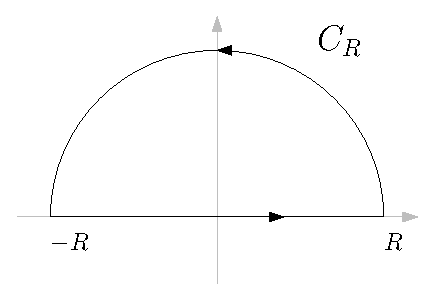
\includegraphics[scale=1]{circ.eps}
    \caption{Полукруг в верхней полуплоскости с обходом против часовой стрелки}
		\label{fig:13.1}
\end{figure}
\\
Пусть 
\begin{align*}
  & I_R = \int_{\gamma_R}f(z)dz = 2 \pi i \left( \us{z_0}{\res} f(z) +  \us{z_1}{\res} f(z)\right) = 2 \pi i \left( \left.\frac{1+z^2}{4z^3}\right|_{z_0} + \left.\frac{1+z^2}{4z^3}\right|_{z_1}\right) = 2 \pi i \cdot \\
  & \cdot \left( \frac{1+\exp\left( \frac{2i \pi}{4} \right)}{4 \exp \left( \frac{3i \pi}{4} \right)} +  \frac{1+\exp\left( \frac{6i \pi}{4} \right)}{4 \exp \left( \frac{9i \pi}{4} \right)}\right) = 2 \pi i \left( \frac{\exp\left( \frac{-i\pi}{4} \right) + \exp\left( \frac{i\pi}{4} \right)}{2 i \cdot 2} +  \frac{\exp\left( \frac{-3i\pi}{4} \right) + \exp\left( \frac{3i\pi}{4} \right)}{-2 i \cdot 2}\right) = \\
  & = \pi \left( \cos \frac{\pi}{4} - \cos \frac{3\pi}{4} \right) = \pi \sqrt{2}
\end{align*}
\begin{align*}
  & \pi \sqrt{2} = \int_{-R}^{+R}f(z) + \int_{C_R}f(z) \us{R\to \infty}{\longrightarrow} \int_{-\infty}^{+\infty} f(z) = \int_{-\infty}^{\infty}f(x)
\end{align*}
Итак, достаточно доказать
\begin{align*}
  & \int_{C_R}f(z)  \us{R\to \infty}{\longrightarrow} 0
\end{align*}
чтобы получить, что $I = \pi \sqrt{2}$.
    \begin{flushright}
    \textit{Лекция 10 (от 06.10)}
\end{flushright}
\section{$\S 14.$ Приращение аргумента $z$ вдоль кривой}


    \newpage
\section{Лекционные задачи.}
Автор решения многих задач: \href{https://vk.com/h0ho_haha}{Лев Нечитайло}.

\subsection{Различные системы множеств.}
\newpage
\lecture{1}{Различные системы множеств.}

В этом курсе имеется дело с функциями, аргументами которых являются множества.
\begin{definition}
	\mdef{Мерой} на множестве $X$ называется функция
	$\mu:\: \F \rightarrow [0,\, \infty]$, где $\F$~--- семейство подмножеств $X$.
\end{definition}

На $\F$ нужно наложить некоторые ограничения, потому как если, к примеру, определена мера для двух множеств,
то логично было бы, чтобы была определена мера и на их сумме, пересечении, объединении. Отсюда вытекают такие понятия как:

\begin{definition}
	Семейство $\F$ подмножеств множества $X$ (далее используется обозначение $\F \subset \mathcal{P} (X)\equiv 2^{X}$, где
	$\mathcal{P} (X)$~--- множество всех подмножеств множества $X$) называется \mdef{$\sigma$"=алгеброй}, если
	\begin{enumerate}[label=\arabic*\degree.]
		\item $\varnothing\in \F$.
		\item $\forall A,\, B\in\F:\: A\cap B\in\F,\,A\cup B\in\F,\, A\setminus B\equiv A\cap B^C\in\F$, где
		      $B^C=X\setminus B$.
		\item $X\in\F$.
		\item $\forall \{A_n\}_{n\in\N}\subset\F$ выполнено, что
		      $\bigcup\limits_{n=1}^{\infty}A_n\in\F,\,\bigcap\limits_{n=1}^{\infty}A_n\in\F$.
	\end{enumerate}
\end{definition}

\begin{definition}
	$\F$~--- \mdef{кольцо}, если выполняются условия $1\degree$ и $2\degree$.
\end{definition}
\begin{definition}
	$\F$~--- \mdef{алгебра}, если выполняются условия $1\degree$, $2\degree$ и $3\degree$.
\end{definition}

\begin{remark}
	Пусть $\F$~--- $\sigma$"=алгебра, тогда $\forall A\in\F:\: A^C=X\setminus A\in\F$. Тогда
	\[
		\bigcup\limits_{n=1}^{\infty}A_n=\left(\bigcup\limits_{n=1}^{\infty}A_n\right)^{CC}=
		\left(\bigcap\limits_{n=1}^{\infty}A_n^C\right)^C.
	\]
	Поэтому можно сказать, что вторая часть в условии $4\degree$ избыточна. Абсолютно аналогично и в обратную сторону,
	то есть эти два требования равносильны.
	\label{lect1remark1}
\end{remark}

\begin{remark}
	Пусть $\F$~--- кольцо,
	тогда $A\cap B=A\cap\left(B^{CC}\right)=A\setminus B^C=A\setminus\left(X\setminus B\right)=
		A\setminus\left(A\setminus B\right)$. То есть требование замкнутости по пересечению в свойстве $2\degree$ избыточно.
\end{remark}

\begin{exercise}
	Пусть $\F$~--- семейство всех ограниченных подмножеств множества $\R$. Тогда $\F$~--- кольцо, но не алгебра.
\end{exercise}

\begin{definition}
	Кольцо $\F$ называется
	\begin{enumerate}[label=\alph*)]
		\item \mdef{$\sigma$"=кольцом}, если $\forall \{A_n\}_{n=1}^{\infty}\subset\F$ выполнено, что
		      $\bigcup\limits_{n=1}^{\infty}A_n\in\F$.
		\item \mdef{$\delta$"=кольцом}, если $\forall \{A_n\}_{n=1}^{\infty}\subset\F$ выполнено, что
		      $\bigcap\limits_{n=1}^{\infty}A_n\in\F$.
	\end{enumerate}
\end{definition}

\begin{remark}
	Любое $\sigma$"=кольцо является $\delta$"=кольцом, но обратное неверно.
\end{remark}

\begin{definition}
	Множество $I\subset \R$ называется \mdef{промежутком}, если $\forall a,\, b\in I:\: [a,\, b]\subset I$.
	Промежуток $I$ называется \mdef{конечным}, если он ограничен.

	Например, $[a,\, b],\, (a,\, b),\, [a,\, b),\, (a,\, b]$~--- промежутки.
\end{definition}

Пусть $K_1$~--- семейство всех конечных промежутков на прямой. Легко заметить, что это не кольцо (объединение промежутков
--- не всегда промежуток). Отсюда вытекает новая структура:

\begin{definition}
	Семейство $\F\subset \mathcal{P} (X)$ называется \mdef{полукольцом}, если
	\begin{enumerate}[label=\arabic*\degree.]
		\item $\varnothing\in \F$.
		\item $\forall A,\, B\in\F:\: A\cap B\in\F$, а $A\setminus B$ представимо в виде
		      конечного дизъюнктного объединения элементов $\F$, то есть
		      \[\exists n\in\N: \: \exists A_1,A_2,\ldots,A_n\in\F: \: A\setminus B=\bigcup_{i=1}^{n}A_i
			      ,\, A_i\cap A_j=\varnothing,\, \forall i,j: i\neq j.\]
		      Если множества попарно не пересекаются, то вводиться обозначение:
		      \[A_1\cup A_2\cup\ldots\cup A_n=A_1\sqcup A_2\sqcup\ldots\sqcup A_n.\]
	\end{enumerate}
\end{definition}

\begin{remark}
	Для любого семейства множеств $\F$ под $\FDU(\F)$ будем понимать семейство всех конечных дизъюнктных
	объединений элементов $\F$ (FDU~--- finite disjoint union).
\end{remark}

\begin{claim}
	$K_1$~--- полукольцо.
\end{claim}

\begin{definition}
	$K_d=\{I_1\times I_2\times \ldots\times I_d,\, \text{где } I_l\in K_1\quad\forall l = \overline{1..d}\}$, $d\in\N$~--- \mdef{семейство клеток
	в $\R^d$}.
\end{definition}

\begin{claim}
	$K_d$~--- полукольцо.
\end{claim}

\begin{definition}
	Пусть $\F$~--- семейство подмножеств множества $X$.
	Введем обозначение: \[\mathcal{R}(\F):=\bigcap\{\mathcal{G}:\:\mathcal{G}\text{~--- кольцо, } \F\in\mathcal{G} \}:=\bigcap M.\]
	$\mathcal{R}(\F)$ называется \mdef{кольцом порожденным $\F$}.
\end{definition}

\begin{theorem}
	\label{lect1thdef}
	$\mathcal{R}(\F)$ является кольцом и $\F\subset \mathcal{R}(\F)$. При этом $\mathcal{R}(\F)$~--- наименьшее по вложению кольцо $\mathcal{S} $,
	такое что $\F\subset \mathcal{S}$.

	\begin{proof}
		\textbf{Шаг 1.} $\mathcal{R} $~--- кольцо, так как
		\begin{enumerate}
			\item $\varnothing\in \mathcal{R}:\: \forall \mathcal{G}$ выполнено $\varnothing\in\mathcal{G}$.
			\item $\forall A,\, B$ верно, что $A,\, B\in \mathcal{G} $, но $\mathcal{G} $~--- кольцо, поэтому
			      $A\cup B\in\mathcal{G} $ и $A\setminus B\in\mathcal{G}$. Таким образом и пересечению данные множества принадлежат.
		\end{enumerate}

		\textbf{Шаг 2.} Если $\mathcal{S} $~--- кольцо и $\F\subset \mathcal{S} $, то $\mathcal{R} \subset \mathcal{S}$, так как
		$\mathcal{S} \in M\Rightarrow \bigcap M\subset \mathcal{S} .$

	\end{proof}
\end{theorem}

\begin{remark}
	Доказательство основано на том факте, что если $\F$ и $\mathcal{G}$~--- кольца, то $\F\cap \mathcal{G} $~--- тоже кольцо.
\end{remark}

Опишем структуру кольца, порожденного полукольцом.

\begin{theorem}
	Пусть $\mathcal{S} $~--- полукольцо. Тогда
	\[
		\mathcal{R} (\mathcal{S} )=\left\{\bigsqcup_{l=1}^{n}A_l:\: n\in\N,\, A_1,\ldots, A_n\in\mathcal{S},\, A_i\cap A_j=\varnothing:
		\: i\neq j\right\} = \FDU(\mathcal{S} ).
	\]
	\label{lect1th1}
\end{theorem}

\begin{lemma} Ослабим условие теоремы выше. Тогда все равно:
	\[
		\mathcal{R} (\mathcal{S} )=\left\{\bigcup_{l=1}^{n}A_l:\: n\in\N,\, A_i\in\mathcal{S}: \: \forall i=\overline{1..n}\right\}
		\cup\{\varnothing\}.
	\]

	\begin{proof}
		Пусть $R=\left\{\bigcup_{l=1}^{n}A_l:\: n\in\N,\, A_i\in\mathcal{S}: \: \forall i=\overline{1..n}\right\}$. Ясно, что
		$R\subset \mathcal{R} (\mathcal{S} )$. Докажем в обратную сторону. Для этого достаточно доказать, что $R$~--- кольцо, тогда
		сразу выполнится $\mathcal{R} (\mathcal{S} )\subset R$.

		Пустое множество очевидно лежит в $R\cup\{\varnothing\}$.

		Пусть $P=\bigcup\limits_{k=1}^{n}A_k,\, A_k\in\mathcal{S} $ и $Q=\bigcup\limits_{l=1}^{m}B_l,\, B_l\in\mathcal{S} $. Тогда, во-первых,
		\[P\cup Q=A_1\cup A_2\cup\ldots\cup A_n\cup B_1\cup B_2\cup\ldots\cup B_m\in R.\]
		Во-вторых,
		\begin{align*}
			P\setminus Q & =\bigcup_{k=1}^{n}\left(A_k\setminus \bigcup_{l=1}^m B_{l}\right)=
			\bigcup_{k=1}^{n}\left(A_k\bigcap \left(\bigcup_{l=1}^m B_{l}\right)^C\right)=                 \\
			             & =\bigcup_{k=1}^{n}\left(A_k\bigcap \left(\bigcap_{l=1}^m B_{l}^C\right)\right)=
			\bigcup_{k=1}^{n}\bigcap_{l=1}^{m}A_k\cap B_l^C=
			\bigcup_{k=1}^{n}\bigcap_{l=1}^{m}A_k\setminus B_l.
		\end{align*}

		Далее имеем $A_k,\, B_l\in \mathcal{S} \Rightarrow A_k\setminus B_l\in \FDU(\mathcal{S})\Rightarrow A_k\setminus
			B_l=\bigsqcup\limits_{i=1}^{N_{k,l}}S_i\Rightarrow \bigcap\limits_{l=1}^{m}A_k\setminus B_l\in\FDU(\mathcal{S} ).$


	\end{proof}
	\label{lect1lemma1}
\end{lemma}
\newpage
\lecture{2}{Параллельные алгоритмы, машинные числа, QR-разложение.}

\subsection{Параллельные вычисления.}

В прошлой лекции изучались такие понятия как алгоритм и его сложность. Как известно в настоящее время существуют устройства, которые
могут выполнять несколько операций за раз и, следовательно, хотелось бы анализировать сложность алгоритмов, выполняющихся данными
устройствами.

\begin{definition}
    \mdef{Параллельная сложность}~--- число параллельных шагов алгоритма, то есть шагов, за которые выполняются разом группа
    операций (параллельно).
\end{definition}

\begin{exercise}
    Зададимся вопросом, какова параллельная сложность алгоритма поиска LU-разложения. Первое наблюдение: когда обнуляется некоторый столбец, понятно, что
    обнулять каждую строчку можно независимо. Более того, при умножении строки на число и вычитании двух строк каждый элемент также можно считать независимо.
    А значит для обнуления одного столбца требуется один шаг, а значит общая параллельная сложность порядка $n$ (как и в прошлый раз $n$~--- порядок матрицы).
\end{exercise}

\begin{exercise}
    Применив аналогичные рассуждения, можно найти еще параллельную сложность поиска решения системы
    уравнений $Ux=b$, где $U$~--- верхняя треугольная матрица. Понятно, что в данном случае параллельная сложность составит тоже $\Theta(n)$.
\end{exercise}

\begin{remark}
    Стоит помнить, что несмотря на то, что много операций можно выполнить за раз, для каждой группы операций нужны какие-то
    данные, которые возможно не успели еще посчитаться, а значит какие-то шаги могут простаивать и ждать пока данные будут подготовлены,
    то есть возникает так называемая гонка за данными.
\end{remark}

\subsection{Представление чисел в компьютере.}

Машинные числа имеют вид:
\[
    10 ^ {p}  \cdot \overbrace{0.\underbrace{****\ldots **}_{t \text{ разрядов.}}}^{\text{мантисса}}, \quad p\text{~--- порядок.}
\]

Обычно количество разрядов $t$ фиксированно и порядок $p$ ограничен каким-то числом: $|p|\leqslant p_{\max}$, то есть не все вещественные числа
представляются таким образом, в том числе следует помнить, что при вычислениях получается именно машинное число, то есть не всегда
результат выражения совпадает с истинным (с точки зрения математики) ответом.

В силу этого появляется некая погрешность, о которой следует помнить.
\begin{exercise}
    Возьмем $t=3$. Что будет результатом вычисления $10^4+1$? Для начала каждое число нужно представить в экспоненциальной
    форме\footnote{форма в которой и представлены машинные числа.}. Итак, $10^4=10^5\cdot 0.100$, $1 = 10^1\cdot 0.100$.
    Чтобы найти сумму, нужно сравнять порядки чисел, в данном случае привести единицу к порядку 5, то есть представить в виде
    $10^5\cdot 0.00001$, но так как у нас число разрядов равно 3, то единица в 5"=ом знаке просто не вместится и число станет нулем.
    Тогда итоговое значение будет $10^4+1=10^4$, что конечно же противоречит истинному.

    \textbf{Вывод}: часто, если складываются очень большое и очень маленькое числа, вполне вероятно, что произойдет такая ситуация.
\end{exercise}

Попробуем теперь найти LU-разложение матрицы с учетом данного аспекта.

\begin{exercise}
    Пусть
    \[
        A = \left(
        \begin{array}{cc}
                10^{-t} & 1 \\
                1       & 1
            \end{array}
        \right),\quad t\text{~--- число разрядов.}
    \]

    Итак, обнуляем первый столбец (большое по модулю число $10^t$ <<съедает>> маленькую единицу в матрицах $L$ и $U$):
    \[
        U = \left(
        \begin{array}{cc}
                10^{-t} & 1      \\
                0       & 1-10^t
            \end{array}
        \right)=\left(
        \begin{array}{cc}
                10^{-t} & 1     \\
                0       & -10^t
            \end{array}
        \right), \quad L =\left(
        \begin{array}{cc}
                1    & 0 \\
                10^t & 1
            \end{array}
        \right).
    \]

    Давайте найдем $LU$:
    \[
        LU=\left(
        \begin{array}{cc}
                10^{-t} & 1 \\
                1       & 0
            \end{array}
        \right) = A - \underbrace{\left(
            \begin{array}{cc}
                0 & 0 \\
                0 & 1
            \end{array}
            \right)}_{\text{погрешность}}.
    \]
\end{exercise}

\subsection{Проблемы роста.}

Можно заметить, что проблема возникает из-за ведущего числа, которое сильно отличается от остальных. Формализуем машинные вычисления.
\begin{definition}
    Будем писать \mdef{$\fl(expr)$}~--- \textit{машинный} результат вычисления выражения $expr$.
    Например, на машине с $t=3: \fl(10^4+1)=10^4$.
\end{definition}

Итак, введем аксиому машинной арифметики:
\begin{axiom}[машинной арифметики]
    \[
        \fl(a\cdot b) = a\cdot b\cdot (1+\varepsilon), \quad |\varepsilon|\leqslant\eta\text{~--- <<машинный нуль>>}.
    \]
\end{axiom}

Если данная аксиома выполнена, можно рассмотреть теорему:

\begin{theorem}
    Пусть $\widetilde{L},\, \widetilde{U}$~--- машинные матрицы. Тогда \[\left|A-\widetilde{L}
        \cdot\widetilde{U}\right|\leqslant cn\eta\left(\left|A\right|+\left|\widetilde{L}\right|\cdot\left|\widetilde{U}\right|\right)+O(\eta^2),\]
    где $c$~--- некоторая константа.
\end{theorem}

В теореме видно, что большой вклад в погрешность вносят как раз матрицы $\widetilde{L}\text{ и }\widetilde{U}$. Как нужно изменить метод Гаусса, чтобы
ограничить рост элементов этих матриц?

Будем просто на место ведущего элемента выбирать наибольший в столбце, тогда в матрице $\widetilde{L}$ будет верно следующее неравенство:
$\left|\widetilde{L}_{ij}\right|\leqslant 1$. С матрицей $\widetilde{U}$ дела обстоят сложнее. Тем не менее, можно доказать следующее утверждение:
\begin{claim}
    \[
        \max_{i,\,j} \widetilde{U}_{ij}\leqslant 2^{n-1}\cdot \left(\max_{i,\,j} A_{ij}\right).
    \]
\end{claim}

\subsection{Матрицы вращения.}

Как ни удивительно, есть способы вообще избежать роста коэффициентов.
Рассмотрим матрицу:
\[
    Q = \left(
    \begin{array}{cc}
            \cos\varphi & -\sin\varphi \\
            \sin\varphi & \cos\varphi
        \end{array}
    \right), \quad Q^T = \left(
    \begin{array}{cc}
            \cos\varphi  & \sin\varphi \\
            -\sin\varphi & \cos\varphi
        \end{array}
    \right) = Q^{-1}.
\]

$Q$ называется \mdef{матрицей вращения}.

\begin{definition}
    Матрица $A$ называется \mdef{ортогональной}, если $A^TA=I$.
\end{definition}

Понятно, что матрица вращения является ортогональной. Оказывается, что с помощью матрицы вращения
тоже можно исключать значения, к примеру подберем матрицу вращения так, чтобы было выполнено:

\[
    \left(
    \begin{array}{cc}
            \cos\varphi & -\sin\varphi \\
            \sin\varphi & \cos\varphi
        \end{array}
    \right)\cdot
    \left(
    \begin{array}{c}
            a \\
            b
        \end{array}
    \right)=
    \left(
    \begin{array}{c}
            c \\
            0
        \end{array}
    \right).
\]
То есть $a\sin\varphi+b\cos\varphi=0$, понятно, что это всегда можно сделать:

\[
    \sin\varphi=-\dfrac{b}{\sqrt{a^2+b^2}},\quad \cos\varphi=\dfrac{a}{\sqrt{a^2+b^2}}.
\]

Научимся приводить матрицу к диагональному виду, используя этот прием. Но сначала важное понятие:

\begin{definition}
    Матрица $G_{kl}$ называется \mdef{обобщенной матрицей вращения} или
    \mdef{матрицей Гивенса}, если она отличается от единичной матрицей лишь подматрицей $Q$,
    расположенной на строках и столбцах с номерами $k$ и $l$.

    \[
        G_{kl}=
        \left[\begin{array}{ccccccc}
                1      & \cdots & 0         & \cdots & 0          & \cdots & 0      \\
                \vdots & \ddots & \vdots    &        & \vdots     &        & \vdots \\
                0      & \cdots & \cos \phi & \cdots & -\sin \phi & \cdots & 0      \\
                \vdots &        & \vdots    & \ddots & \vdots     &        & \vdots \\
                0      & \cdots & \sin \phi & \cdots & \cos \phi  & \cdots & 0      \\
                \vdots &        & \vdots    &        & \vdots     & \ddots & \vdots \\
                0      & \cdots & 0         & \cdots & 0          & \cdots & 1
            \end{array}\right]
    \]

    Примеры для лучшего понимания:
    \[
        G_{12}=\left(
        \begin{array}{ccccc}
                \cos & -\sin & 0 & \ldots & 0 \\
                \sin & \cos  & 0 & \ldots & 0 \\
                0    & 0     & 1 & \ldots & 0 \\
                \ldots                        \\
                0    & 0     & 0 & \ldots & 1
            \end{array}
        \right),\,
        G_{23}=\left(
        \begin{array}{ccccc}
                1 & 0    & 0     & \ldots & 0 \\
                0 & \cos & -\sin & \ldots & 0 \\
                0 & \sin & \cos  & \ldots & 0 \\
                \ldots                        \\
                0 & 0    & 0     & \ldots & 1
            \end{array}
        \right),\,\ldots
    \]
\end{definition}

Тогда умножив на некоторое число таких матриц (примерно $n^2$~--- столько же, сколько нужно сделать нулей)
получим треугольную матрицу: $Q_s\cdot \ldots \cdot Q_1\cdot A = U$, причем $Q_i=G_{k_i l_{i}}$~--- 
ортогональная матрица для всех $i$, поэтому
\[
    A = Q_{1}^{-1}\cdot\ldots Q_{s}^{-1}\cdot U = Q_{1}^{T}\cdot\ldots Q_{s}^{T}\cdot U\Rightarrow A = QU.
\]

\begin{claim}
    Произведение ортогональных матриц и обратная к ортогональной матрице являются ортогональными матрицами.

    \begin{proof}
        Пусть $A,\, B$~--- ортогональные, тогда
        \begin{enumerate}
            \item $(A^{-1})^TA^{-1}=(A^T)^{-1}A^{-1}=(AA^T)^{-1}=I$;
            \item $(AB)^T(AB) = B^TA^TAB=B^TIB=I$.
        \end{enumerate}
    \end{proof}
\end{claim}

\begin{definition}
    Построенное разложение матрицы называется \mdef{QR-разложением}. То есть матрица $A$
    имеет QR-разложение, если $A=QR$, где $Q$~--- ортогональная матрица, $R$~--- верхняя треугольная матрица.
\end{definition}

\begin{theorem}
    Для любой квадратной вещественной матрицы существует QR"=разложение.
\end{theorem}

Пусть $Q$~--- ортогональная матрица порядка $n$, значит по определению $Q^TQ=I$. Заметим, что 
$(Q^TQ)_{ij}=q^T_{i}q_j=(q_j,\, q_i)$~--- скалярное произведение. Более того
столбцы (и, конечно, строки) матрицы образуют ортонормированную систему, то есть 
\[
    (q_j,\, q_i)=\delta_{ij}=\begin{cases}
        1,\ i=j,\\
        0,\ i\neq j.
    \end{cases}\text{~--- символ Кронекера.}
\]

\begin{claim}
    Пусть есть линейно независимые столбцы: $\vect{a_1},\,\ldots,\,\vect{a_n}\in\R^n$. Утверждается, что 
    от них можно перейти к неким ортонормированным столбцам: $\vect{q_1},\,\ldots,\,\vect{q_n}$ с дополнительным свойством
    $L(\vect{q_1},\,\ldots,\,\vect{q_k})=L(\vect{a_1},\,\ldots,\,\vect{a_k})\ \forall k: 1\leqslant k\leqslant n$, где $L$~--- линейная
    оболочка векторов.

    \begin{proof}
        Доказательство использует важное понятие как процесс ортогонализации Грама-Шмидта: 
        \begin{align*}
            \vect{q_1}&=\dfrac{\vect{a_1}}{\|\vect{a_1}\|}\\
            \vect{p_2}&=\vect{a_2}-r_{12}\vect{q_1},\quad r_{12}=(\vect{a_2},\,\vect{q_1}),\quad 
            \vect{q_2}=\dfrac{\vect{p_2}}{\|\vect{p_2}\|}\\
            \ldots
        \end{align*}

    \end{proof}
\end{claim}

\begin{remark}
    Соответственно для получения QR-разложения матрицы $A$ используем процесс ортогонализации Грама-Шмидта: 
    новые столбцы составят матрицу $Q$, а коэффициенты $r_{ij}$ составят матрицу $R$.
\end{remark}

\begin{claim}
    Пусть $Q$~--- ортогональная матрицы. Тогда $\forall \vect{x}\in\R^n$ выполнено $\|Q\vect{x}\|=\|\vect{x}\|$.
    То есть при умножении вектора на ортогональную матрицу его длина не меняется.

    \begin{proof}
        \[\|Q\vect{x}\|=\sqrt{(Q\vect{x})^T(Q\vect{x})}=\sqrt{\vect{x}^TQ^TQx}=\|\vect{x}\|.\]

    \end{proof}
\end{claim}

\begin{next0}
    При умножении матрицы $A$ слева и справа на ортогональные матрицы сумма квадратов всех элементов 
    сохраняется.
\end{next0}

\begin{exercise}
    Пусть $A$~--- невырожденная нижняя треугольная матрица. Постройте алгоритм вычисления обратной матрицы $A^{-1}$
    с числом параллельных шагов $O(\log_2^2n)$.

    \textbf{Hint:} \mdef{Схема сдваивания.} Пусть требуется сложить $n$ чисел: 
    \[
        S = \underbrace{a_1+a_2}+\underbrace{a_3+a_4}+\underbrace{a_5+a_6}+\underbrace{\ldots+a_n}.   
    \]
    Если их разбить на пары и в каждой паре найти результат независимо, а потом применить такое же рассуждение 
    для результатов, то всего будет порядка $\log_2 n$ шагов.

    \begin{remark}
        Открытой проблемой является вопрос о существовании алгоритма с меньшей параллельной сложностью.
    \end{remark}
\end{exercise}

\begin{remark}
    Более того, известно, что произвольную невырожденную матрицу можно обратить, затратив $O(\log_2^2 n)$ 
    параллельных шагов.        
\end{remark}


\newpage
\lecture{3}{Нормальные процессы, винеровский процесс}
\subsection{Обобщения пуассоновского процесса}
Пуассоновский процесс можно записать как
\begin{align*}
  & K(t) = \sum_{i=1}^{K(t)} 1
\end{align*}
\begin{Def}
    Процесс
    \begin{align*}
      & K_C(t) = \sum_{i=1}^{K(t)} \xi_i
    \end{align*}
    где $\xi_i$ независимы в совокупности и от $K(t)$, называется \textbf{сложным пуассоновским процессом (compound Poisson process)}.
\end{Def}
\begin{Prop}
    Сложный пуассоновский процесс, где $\xi_i \in Be(p)$, будет пуассоновским процессом с интенсивностью $\lambda p$.
\end{Prop}
\begin{Def}
    Если в определении пуассоновского процесса заменить третий пункт на
    \begin{align*}
      & K(t) - K(s) \in Po\left(\int_t^s \lambda(\tau) d\tau\right)
    \end{align*}
    то это называется \textbf{неоднородным пуассоновским процессом}.
\end{Def}
\section{Нормальные (гауссовские) процессы}
\subsection{Нормальные (гауссовские) процессы}
\begin{Def}
    Случайный процесс называется \textbf{нормальным (гауссовским) процессом}, если все его конечномерные распределения гауссовские, то есть
    \begin{align*}
      & \forall n \in \NN \ \left(X(t_1), \dots, X(t_n)\right)
    \end{align*}
    имеют нормальное распределение.
\end{Def}
\begin{Def}
    Cлучайный вектор
    \begin{align*}
      & \forall n \in \NN \ \left(X(t_1), \dots, X(t_n)\right)
    \end{align*}
    \textbf{имеет нормальное распределение}, если
    \begin{align*}
      & \varphi_X(s) = \exp\left(i\mu^T s - \frac{1}{2}s^TRs\right), \ s \in \RR^n
    \end{align*}
    \begin{align*}
      & \mu = \EE X \in \RR^n, \ R = \EE\left( \cent{X}\cent{X}^T \right)
    \end{align*}
    Говорят, что
    \begin{align*}
      & X \in \cN(\mu, R)
    \end{align*}  
\end{Def}
\textbf{Свойства нормального вектора}
\begin{enumerate}
    \item Покомпонентно
    \begin{align*}
      & X \in \cN(\mu, R) \Rightarrow X_i \in \cN(\mu_i, R_{ii})
    \end{align*}
    А если все компоненты независимы, то верно и обратное.
    \item Если
    \begin{align*}
      & X \in \cN(\mu, R), \ \det R \neq 0
    \end{align*}
    то существует плотность распределения
    \begin{align*}
      & f(x) = \frac{1}{(2\pi)^{\frac{n}{2}}\sqrt{\det R}}\exp \left( -\frac{1}{2}(x-\mu)^TR^{-1}(x-\mu) \right), \ x \in \RR^n
    \end{align*}
    Если матрица вырождена, то плотности у вектора нет. В случае вырожденности
    есть линейно зависимые компоненты в векторе. Действительно, в этом случае
    \begin{align*}
      & \exists c \neq 0: Rc = 0;
    \end{align*}
    \begin{align*}
      & Rc = 0 \Rightarrow c^TRc = 0 \Rightarrow 0 = c^T \EE \cent{X}\cent{X}^Tc = \EE c^T \cent{X}\cent{X}^Tc = \EE\left( \cent{X}^Tc \right)^2 = 0 \Rightarrow \cent{X}^Tc = 0
    \end{align*}
    \item Пусть
    \begin{align*}
      & X \in \cN(\mu, R), \ X \in \RR^n
    \end{align*}
    Тогда
    \begin{align*}
      & \forall A \in \RR^{k\times n} AX \in \cN(A\mu, ARA^T)
    \end{align*}
    \item Вектор $X$ нормален тогда и только тогда, когда $\forall \{c_i\} \
    \sum c_ix_i$~--- нормальная (или константа, но константа~--- частный случай
    нормальной величины.)
    \item Компоненты нормального случайного вектора некоррелированы тогда и
    только тогда, когда независимы.
    \item Условные распределения подвекторов нормального вектора нормальны.
    \begin{align*}
      & X = \left( \xi, \eta \right) \in \cN(\mu, R), \ X \in \RR^{n+m}, \ \xi \in \RR^n, \ \eta \in \RR^m
    \end{align*}
    \begin{align*}
      & \mu = \left[ \begin{matrix}
              \mu_{\xi} \\
              \mu_{\eta}
          \end{matrix} \right], \ R = \left[ \begin{matrix}
              R_{\xi \xi} & R_{\xi \eta} \\
              R_{\eta \xi} & R_{\eta \eta}
          \end{matrix} \right]
    \end{align*}
    Пусть $\det R_{\eta \eta} \neq 0$, тогда
    \begin{align*}
      & \left( \xi \mid \eta = x \right) \in \cN\left( \mu_{\xi} + R_{\xi \eta}R^{-1}_{\eta \eta}(x-\mu\eta), R_{\xi \xi}-R_{\xi \eta}R_{\eta \eta}^{-1}R_{\eta \xi}\right)
    \end{align*}    
\end{enumerate}
\subsection{Винеровский процесс}
\begin{Def}
    Cлучайный процесс $\{W(t), \ t \geq 0\}$ называется \textbf{винеровским
      (процессом броуновского движения)}, если
    \begin{enumerate}
        \item $W(0) = 0$ п.~н.
        \item это процесс с независимыми приращениями
        \item $\forall t, s \geq 0 \ W(t) - W(s) \in \cN(0, \left| t-s \right|)$
    \end{enumerate}
\end{Def}
\begin{Def}
    Cлучайный процесс $\{W(t), \ t \geq 0\}$ называется \textbf{винеровским с
      параметром $\sigma^2$}, если его определение отличается от винеровского
    лишь третьим пунктом:
    \\
    $\forall t, s \geq 0 \ W(t) - W(s) \in \cN(0, \sigma^2 \left| t-s \right|)$
\end{Def}
\begin{theorem}
    Винеровский процесс является нормальным.
\end{theorem}
\begin{Proof}
    Пусть $\forall n \geq 1$ рассмотрим числа $t_1\leq t_2\leq \dots \leq t_n
    \in \RR_+$.
     \begin{align*}
      & X = \left(W(t_1), \dots, W(t_n)\right); \ W(t) = W(t) - W(0) \in \cN(0, t)
     \end{align*}
      \begin{align*}
      & W(t_j) - W(t_{j-1}) \in \cN(0, t_j-t_{j-1})
      \end{align*}
      Они независимы в совокупности, и вектор
      \begin{align*}
        Y = \left[ \begin{matrix}
                W(t_1) - W(0) \\
                W(t_2) - W(t_1) \\
                \dots \\
                W(t_n) - W(t_{n-1})
            \end{matrix} \right]
      \end{align*} 
    \begin{align*}
      & X =\left[ \begin{matrix}
              1 & 0 & \dots & 0 \\
              1 & 1 & \dots & 0 \\
              \dots & \dots & \dots & \dots \\
              1 & 1 & \dots & 1
          \end{matrix} \right] Y
    \end{align*}
    Тогда это нормальный вектор.
    \\
    Если неупорядочены $t_i$~--- то можно упорядочить это линейным преобразованием.
\end{Proof}
Пуассоновский, винеровский и другие процессы называются \textbf{процессами
  Леви}~--- процессами со стационарными независимыми приращениями. Всякий такой
процесс есть композиция нормального и сложного пуассоновского.
\begin{Prop}
    Почти все траектории винеровского процесса всюду непрерывны, но нигде не дифференцируемы.
\end{Prop}
\begin{Prop}
    \begin{align*}
      & \EE W(t) = 0, \ R_W(t,s) = \min(t,s)
    \end{align*}
\end{Prop}
\begin{theorem} Вика (без доказательства)
    \\
    Пусть
    \begin{align*}
      & (X_1, X_2, \dots, X_n) \in \cN (0, R)
    \end{align*}
    Тогда если $n$ нечетно, то
    \begin{align*}
      & \EE X_1X_2\dots X_n = 0
    \end{align*}
    Если же $n$ четно, тогда
    \begin{align*}
      & \EE X_1X_2\dots X_n = \sum R_{p_1q_1}\dots R_{p_{\frac{n}{2}}}
    \end{align*}
    где сумма берется по всем неупорядоченным разбиениям $\{1, \dots, n\}$ на
    $\dst \frac{n}{2}$ неупорядоченных пар.
\end{theorem}
\begin{example}
    \begin{align*}
      & X = \left( X_1, \dots, X_n \right) \in \cN(0, R)
    \end{align*}
    \begin{align*}
      & \EE X_1 = 0, \ \EE X_1X_2X_3 = 0, \ \EE X_1^3 = 0, \ \EE X_1^2X_2^3 = 0
    \end{align*}
    \begin{align*}
      & \EE X_1X_2X_3X_4 = R_{12}R_{34} +R_{13}R_{24} + R_{14}R_{23}
    \end{align*}
    \begin{align*}
      & 12 \mid 34 \sim 34 \mid 12, \ 12 \mid 34 \sim 21 \mid 43
    \end{align*}
\end{example}
\begin{example}
    \begin{align*}
      & \EE W^4(t)
    \end{align*}
    \begin{align*}
      & X = \left( X_1, X_2, X_3, X_4 \right)^T = \left( W(t), W(t), W(t), W(t) \right)^T
    \end{align*}
    \begin{align*}
      & \EE W^4(t) = \EE X_1X_2X_3X_4 = R_{12}R_{34} +R_{13}R_{24} + R_{14}R_{23} = 3 \cov(W(t),W(t))^2 = 3t^2
    \end{align*}
\end{example}
\subsection{Случайные блуждания и винеровский процесс}
\begin{Def}
    Пусть
    \begin{align*}
      & S_n = \sum_{i=1}^n \xi_i
    \end{align*}
    где $\{\xi_i\}$ независимы в совокупности. Такие процессы называются
    \textbf{случайными блужданиями.}
\end{Def}
\begin{theorem} ~
    \\
    Пусть
    \begin{align*}
      & \{\xi_i\} \ \IID, \ \EE \xi_i = 0, \ \DD \xi_i = \sigma^2
    \end{align*}
    Тогда конечномерные распределения процесса
    \begin{align*}
      & X_n (t) = \frac{1}{\sigma \sqrt{n}} \sum_{k=1}^{\left[ nt \right]} \xi_k
    \end{align*}
    сходятся к конечномерным распределениям винеровского процесса.
    \\
    Считаем, что $X_n(t) = 0$ при $[nt]=0$.
\end{theorem}
\begin{Proof}
    Заметим, что
    \begin{align*}
      & \frac{1}{\sigma \sqrt{n}}S_{[nt]} \us{n \to \infty}{\os{d}{\to}} W(t)
    \end{align*}
    Рассмотрим $s<t$.
    \begin{align*}
      & \left( X_n(t), X_n(s) \right) \us{n \to \infty}{\os{d}{\to}} (W(s), W(t))
    \end{align*}
    \begin{align*}
      & \left( X_n(t), X_n(t) - X_n(s) \right) \us{n \to \infty}{\os{d}{\to}} (W(s), W(t)-W(s))
    \end{align*}
    Утверждения равносильны, поскольку из теории вероятностей известно:
    \begin{align*}
      & \left( \xi_n, \eta_n \right) \us{n \to \infty}{\os{d}{\to}} (\xi, \eta) \Leftrightarrow \left( \xi_n, \xi_n + \eta_n \right) \us{n \to \infty}{\os{d}{\to}} (\xi, \xi+\eta)
    \end{align*}
    Второе утверждение:
    \begin{align*}
      & \left( \frac{1}{\sigma \sqrt{n}}S_{[ns]}, \frac{1}{\sigma \sqrt{n}}S_{[nt]} - \frac{1}{\sigma \sqrt{n}}S_{[ns]} \right) \us{n \to \infty}{\os{d}{\to}} \left( W(s), W(t)-W(s) \right)
    \end{align*}
    Имеем право так делать, поскольку правая и левая части независимы.
    \\
    Аналогично, выражая все через приращения, сможем выразить все многомерные распределения.
\end{Proof}
\newpage
\lecture{4}{Стохастический анализ}
\section{Стохастический анализ}
Непрерывность, дифференцируемость и интегрируемовть процессов рассматривается по
времени, исход рассматривают как параметр.
\\
Вспомним сходимости случайных величин:
\begin{itemize}
    \item в среднеквадратичном
    \item почти наверное
    \item по вероятности
    \item по распределению
\end{itemize}
\subsection{Сходимость}
\begin{Def}
    Говорят, что последовательность случайных величин $X_n$ \textbf{сходится в
      среднеквадратичном смысле} к случайной величине $X$:
    \begin{align*}
      & X_n \tosk{n \to \infty} X \Leftrightarrow X = \LIM{n \to \infty} X_n \Leftrightarrow \lim_{n \to \infty} \EE(X_n- X)^2 = 0
    \end{align*}
\end{Def}
\begin{lemma}
    ~
    \\
    Пусть $\left\{ X_m \right\}_{m = 1}^\infty$, $\left\{ Y_n \right\}_{n =
      1}^\infty$~--- случайные величины, заданные на одном вероятностном
    пространстве. \textit{Это подразумевается, если не указано иного.} Тогда
    верно:
    \begin{align*}
      \lim_{n, m \to \infty} \EE X_mY_n = \EE \LIM{m \to \infty} X_m \EE \LIM{n \to \infty} Y_n = \EE XY
    \end{align*}
\end{lemma}
\begin{Proof}
    \begin{align*}
      & X_mY_n - XY = \left( X_m - X \right)\left( Y_n - Y \right) + \left( X_m - X \right)Y + \left( Y_n - Y \right)X
    \end{align*}
    \begin{align*}
      & \left| \EE X_mY_n - \EE XY \right| \leq \left| \EE \left( X_m - X \right)\left( Y_n - Y \right) \right| + \left| \EE \left( X_m - X \right)Y \right| + \left| \EE \left( Y_n - Y \right)X \right|
    \end{align*}
    Применим неравенство Коши-Буняковского.
    \begin{align*}
      & \left| \EE \left( X_m - X \right)\left( Y_n - Y \right) \right| \leq \sqrt{\EE(X_m - X)^2\EE(Y_n - Y)^2} \To{m, n \to \infty} 0
    \end{align*}
    \begin{align*}
      & \left| \EE \left( X_m - X \right)Y \right| \leq \sqrt{\EE(X_m - X)^2\EE Y^2} \To{m \to \infty} 0
    \end{align*}  
    \begin{align*}
      & \left| \EE \left( Y_n - Y \right)X \right| \leq \sqrt{\EE(Y_n - Y)^2\EE X} \To{n \to \infty} 0
    \end{align*}
    Значит,
    \begin{align*}
      & \left| \EE X_mY_n - \EE XY \right| \to 0 \Rightarrow \EE X_mY_m \To{m, n \to \infty} \EE XY
    \end{align*}
\end{Proof}
\begin{Note}
    Если $Y_n \equiv Y \equiv 1$, то
    \begin{align*}
      & X_m \tosk{m \to \infty} X \Rightarrow \EE X_m \To{m \to \infty} \EE X
    \end{align*}
\end{Note}
\begin{lemma}
    (без доказательства)
    \\
    Среднеквадратичная сходимость обладает свойством фундаментальности по Коши.
    \\
    Пусть $\left\{ X_k \right\}_{k=1}^\infty$~--- случайная последовательность,
    причем $\forall k \ \EE X_k^2 < \infty$. Тогда сходимость в СК к некоторой
    случайной величине $X$, $\EE X < \infty$ равносильна тому, что для любых её
    подпоследовательностей $\left\{ Y_n \right\}_{n=1}^{\infty}$, $\left\{ Z_m
    \right\}_{m=1}^\infty$ выполнено
    \begin{align*}
      \LIM{m, n \to \infty}(Y_m - Z_n)^2 = 0
    \end{align*}
\end{lemma}
\begin{lemma}
    ~
    \\
    Пусть
    \begin{align*}
      \left\{ X_k \right\}_{k=1}^\infty, \ \forall k \ \EE X_k^2 < \infty; \ \exists c \in \RR: \ \forall \left\{ Y_n \right\}_{n=1}^\infty, \ \left\{ Z_m \right\}_{m=1}^\infty \ \EE Y_nZ_m \To{m,n \to \infty} c
    \end{align*}
    Тогда существует случайная величина $X$:
    \begin{align*}
      & X_k \tosk{k \to \infty} X, \ \EE X^2 < \infty
    \end{align*}
\end{lemma}
\begin{Proof}
    \begin{align*}
      & \left( Y_m - Z_n \right)^2 = Y_m^2 - 2Y_mZ_n + Z_n^2
    \end{align*}
    \begin{align*}
      & \lim_{m,n \to \infty}\EE\left( Y_m - Z_n \right)^2 = c - 2c + c = 0
    \end{align*}
    По лемме $2$ $X_k$ сходится в СК.
\end{Proof}
\begin{Def}
    процесс $\left\{ X(t), \ t \in T \right\}$ называется \textbf{процессом
      второго порядка} ($L_2$-процессом), если $\forall t \in T \ \EE X^2(t) <
    \infty$.
\end{Def}
\subsection{СК-непрерывность}
\begin{Def}
    Случайный процесс $\left\{ X(t), \ t \in T \right\}$ второго порядка
    называется \textbf{непрерывным в среднеквадратичном смысле} (СК-непрерывным)
    в $t_0$, если
    \begin{align*}
      & X(t_0+\varepsilon) \tosk{\varepsilon \to 0} X(t_0)
    \end{align*}
\end{Def}
\begin{theorem}
    Критерий СК-непрерывности в точке.
    \\
    Процесс $\left\{ X(t), \ t \in T \right\}$ второго порядка СК-непрерывен в
    $t_0$ тогда и только тогда, когда $K_x(t,s)$ непрерывна в $(t_0,t_0)$, что
    равносильно одновременным непрерывности $m_X(t)$ в $t_0$ и $R_X(t,s)$ в
    $(t_0,t_0)$.
\end{theorem}
\begin{Proof}
    ~
    \\
    \begin{itemize}
        \item Первая равносильность.
        \\
        Пусть $X(t)$ СК-непрерывен в $t_0$. Тогда по определению
        \begin{align*}
          & X(t_0 +\varepsilon_1) \tosk{\varepsilon_1 \to 0} X(t_0), \ X(t_0 +\varepsilon_2) \tosk{\varepsilon_2 \to 0} X(t_0)
        \end{align*}
        Из леммы $1$
        \begin{align*}
          & K_X(t_0+\varepsilon_1, t_0+\varepsilon_2) = \EE X(t_0+\varepsilon_1)X(t_0 + \varepsilon_2) \To{\varepsilon_1, \varepsilon_2 \to 0} \EE X^2(t_0) = K_X(t_0,t_0) < \infty
        \end{align*}
        Необходимость непрерывности доказана.
        \\
        Обратно, если ковариационная функция непрерывна, то
        \begin{align*}
          & \EE\left( X(t_0+\varepsilon) - X(t_0) \right)^2 = \EE\left( X(t_0+\varepsilon) - X(t_0) \right)\left( X(t_0+\varepsilon) - X(t_0) \right) = K_X(t_0+\varepsilon, t_0 +\varepsilon) - \\
          & - 2K(t_0+\varepsilon, t_0) + K_X(t_0,t_0) \To{\varepsilon \to 0} 0
        \end{align*}
        По определению это означает СК-непрерывность $X(t)$ в $t_0$.
        \\
        Достаточность непрерывности доказана.
        \item Вторая равносильность.
        \\
        Если $m_X(t)$ непрерывно в $t_0$, как и $R_X(t,s)$ в $(t_0,t_0)$, то в
        силу того, что $K_X(t,s) = R_X(t,s) + m_X(t)m_X(s)$, непрерывно и
        $K_X(t,s)$ в точке $(t_0, t_0)$.
        \\
        Необходимость непрерывности $K_X(t,s)$ доказана.
        \\
        Обратно, если $K_X(t,s)$ непрерывна, то
        \begin{align*}
          & X(t_0+\varepsilon) \tosk{\varepsilon \to 0} X(t_0)
        \end{align*}
        \begin{align*}
          & \EE\left( X(t_0+\varepsilon) - X(t_0) \right)^2 = \EE\left( \cent{X}(t_0+\varepsilon) - \cent{X}(t_0) + m_X(t_0+\varepsilon) - m_X(t_0) \right)^2 = \\
          & = \EE\left( \cent{X}(t_0+\varepsilon) - \cent{X}(t_0)\right)^2 + 2 \EE\left( \cent{X}(t_0+\varepsilon) - \cent{X}(t_0)\right)\left( m_X(t_0+\varepsilon) - m_X(t_0) \right) + \\
          & + \left( m_X(t_0+\varepsilon) - m_X(t_0) \right)^2 = \EE\left( \cent{X}(t_0+\varepsilon) - \cent{X}(t_0)\right)^2 + \left( m_X(t_0+\varepsilon) - m_X(t_0) \right)^2 \To{\varepsilon \to 0} 0
        \end{align*}
        значит, $m_X(t)$ непрерывно в $t_0$;
        \begin{align*}
          & K_{\cent{X}}(t,s) = R_X(t,s)
        \end{align*}
        непрерывно в $(t_0,t_0)$ в силу
        \begin{align*}
          & \cent{X}(t_0+\varepsilon) \tosk{\varepsilon \to 0} \cent{X}(t_0)
        \end{align*}
        значит, $R_X(t,s)$ непрерывна в $(t_0,t_0)$.
        \\
        Достаточность непрерывности $K_X(t,s)$ доказана.
    \end{itemize}
\end{Proof}
\subsection{СК-дифференцируемость}
\begin{Def}
    Случайный процесс $\left\{ X(t), \ t \in T \right\}$ второго порядка
    называется \textbf{дифференцируемым в среднеквадратичном смысле}
    (СК-дифференцируемым) \textbf{в точке $t_0 \in T$}, если существует
    случайная величина $\eta$, $\EE \eta^2 < \infty$:
    \begin{align*}
      & \frac{X(t_0+\varepsilon) - X(t_0)}{\varepsilon} \tosk{\varepsilon \to 0} \eta
    \end{align*}
    Величина $\eta$ называется \textbf{производной в среднеквадратичном смысле}
    (СК-производной) процесса $X(t)$ в точке $t_0$ и обозначается $\eta =
    X'(t_0)$.
\end{Def}
\begin{Def}
    Случайный процесс $\left\{ X(t), \ t \in T \right\}$ второго порядка
    называется \textbf{дифференцируемым в среднеквадратичном смысле}
    (СК-дифференцируемым), если $\forall t_0 \in T$ он дифференцируем в $t_0$.
    Процесс $\eta(t)$ называется его \textbf{СК-производной}.
\end{Def}
\begin{theorem}
    Критерий СК-дифференцируемости в точке.
    \\
    Процесс $\left\{ X(t), \ t \in T \right\}$ второго порядка СК-дифференцируем
    в $t_0$ тогда и только тогда, когда
    \begin{align*}
      & \lim_{^{\varepsilon \to 0}_{\delta \to 0}}\frac{1}{\delta \varepsilon}\left( K_X(t_0+\varepsilon, t_0+\delta) - K_X(t_0+\varepsilon, t_0) - K_X(t_0, t_0+\delta) + K_X(t_0+\varepsilon, t_0+\delta)\right) < \infty
    \end{align*}
    что равносильно одновременным дифференцируемости $m_X$ в $t_0$ и
    существованию
    \begin{align*}
      & \lim_{^{\varepsilon \to 0}_{\delta \to 0}}\frac{1}{\delta \varepsilon}\left( R_X(t_0+\varepsilon, t_0+\delta) - R_X(t_0+\varepsilon, t_0) - R_X(t_0, t_0+\delta) + R_X(t_0+\varepsilon, t_0+\delta)\right) < \infty
    \end{align*}
\end{theorem}
\begin{Proof}
    ~
    \\
    \begin{itemize}
        \item Первая равносильность.
        \\
        Пусть $X(t)$ СК-дифференцируем в $t_0$. Введем обозначения:
        \begin{align*}
          & Y_\varepsilon = \frac{X(t_0+\varepsilon) - X(t_0)}{\varepsilon}, \ Y_\delta = \frac{X(t_0+\delta) - X(t_0)}{\delta}
        \end{align*}
        Заметим, что
        \begin{align*}
          & \EE Y_\varepsilon Y_\delta = \frac{1}{\delta \varepsilon}\left( K_X(t_0+\varepsilon, t_0+\delta) - K_X(t_0+\varepsilon, t_0) - K_X(t_0, t_0+\delta) + K_X(t_0+\varepsilon, t_0+\delta)\right)
        \end{align*}
        \begin{align*}
          & Y_\varepsilon \tosk{\varepsilon \to 0} X'(t_0), \ Y_\delta \tosk{\delta \to 0} X'(t_0)
        \end{align*}
        Тогда по лемме $1$ необходимо
        \begin{align*}
          & \EE Y_\varepsilon Y_\delta \To{^{\varepsilon \to 0}_{\delta \to 0}} \EE (X'(t_0))^2 < \infty
        \end{align*}
        Необходимость конечности предела доказана.
        \\
        Обратно, если предел существует и конечен, то по лемме $3$ существует
        случайная величина $\eta$: $\EE \eta^2 < \infty$, $Y_{\varepsilon}
        \tosk{\varepsilon \to 0} \eta$, что по определению дает
        СК-дифференцируемость в $t_0$.
        \\
        Достаточность конечности предела доказана.
        \item Вторая равносильность.
        \\
        Если $m_X(t)$ дифференцируемо в $t_0$, а предел из условия для
        $R_X(t,s)$ существует, то в силу того, что $K_X(t,s) = R_X(t,s) +
        m_X(t)m_X(s)$, этот предел существует и для $K_X(t,s)$.
        \\
        Необходимость предела для $K_X(t,s)$ доказана.
        \\
        Обратно, если предел существует, то $X(t)$ СК-дифференцируем в $t_0$, а
        значит,
        \begin{align*}
          & \EE\left( Y_\varepsilon - X'(t_0) \right)^2 = \EE \left( \frac{X(t_0 +\varepsilon) - X(t_0)}{\varepsilon} - X'(t_0) \right)^2 = \EE \left( \frac{\cent{X}(t_0 +\varepsilon) - \cent{X}(t_0)}{\varepsilon} - \cent{X'}(t_0) \right)^2 + \\
          & + \EE \left( \frac{m_X(t_0 +\varepsilon) - m_X(t_0)}{\varepsilon} - \EE X'(t_0) \right)^2 \To{\varepsilon \to 0} 0
        \end{align*}
        В силу дифференцируемости $m_X(t)$ в $t_0$ и СК-дифференцируемости
        $\cent{X}(t)$ в $t_0$ предел для $K_{\cent{X}}(t,s)$ конечен в
        $(t_0,t_0)$. Но
        \begin{align*}
          & K_{\cent{X}}(t,s) = R_X(t,s)
        \end{align*}
        значит, предел для $R_X(t,s)$ существует и конечен.
        \\
        Достаточность предела для $K_X(t,s)$ доказана.
    \end{itemize}
\end{Proof}
\begin{Note}
    Достаточным условием существования обобщенной смешанной производной от
    $K_X(t,s)$ в $(t_0,t_0)$ (предела из условия критерия) является
    непрерывность хотя бы одной из смешанных производных
    \begin{align*}
      & \frac{\partial}{\partial t}\left( \frac{\partial}{\partial s} \left( K_X(t,s) \right) \right), \ \frac{\partial}{\partial s}\left( \frac{\partial}{\partial t} \left( K_X(t,s) \right) \right)
    \end{align*}
    в $(t_0,t_0)$. Тогда обе производные равны между собой и с обобщенной.
\end{Note}
\subsection{СК-интегрируемость}
\begin{Def}
    Пусть процесс $\left\{ X(t), \ t \in T \right\}$ второго порядка определен
    на $[a,b] \subseteq T$. Построим разбиение $a = t_0 < t_1 < \dots < t_{n-1}
    < t_n = b$, $\tau_i \in [t_{i-1}, t_i)$; $\Delta = \dst \max_{i \in \{1,
      \dots, n\}}\left| t_i-t_{i-1} \right|$ называется его мелкостью. Выберем
    на каждом $[t_{i-1}, t_i]$ произвольно $\tau_i$. Если при $n \to \infty$,
    $\Delta \to 0$ существует предел в СК
    \begin{align*}
      & \sum_{i=1}^n X(\tau_i)(t_i-t_{i-1}) \tosk{^{\Delta \to 0}_{n \to \infty}} \eta
    \end{align*}
    не зависящий от $\{t_i\}$, $\{\tau_i\}$, то эта величина называется
    \textbf{интегралом Римана в среднеквадратичном смысле от процесса $X(t)$ в
      пределах от $a$ до $b$} (СК интегралом Римана от $X(t)$ от $a$ до $b$) и
    записывается как
    \begin{align*}
      & \eta = \int_a^bX(t) dt
    \end{align*}
    а процесс~--- \textbf{интегрируемым по Риману в среднеквадратичном смысле в
      пределах от $a$ до $b$} (СК-интегрируемым по Риману).
\end{Def}
\begin{theorem}
    Критерий существования интеграла Римана в среднеквадратичном смысле. (без
    доказательства)
    \\
    Процесс $\{X(t), \ t \in T\}$ второго порядка СК-интегрируем по Риману на
    $[a,b] \subseteq T$ тогда и только тогда, когда существует конечный интеграл
    Римана
    \begin{align*}
      & \int_a^b\int_a^b K_X(t,s) dt ds
    \end{align*}
    что равносильно существованию конечных интегралов Римана
    \begin{align*}
      & \int_a^b\int_a^b R_X(t,s) dt ds, \ \int_a^b m_X(t) dt
    \end{align*}  
\end{theorem}
\begin{Note}
    Определение интеграла Римана в СК от $X$ обобщается на несобственный случай
    следующим образом:
    \begin{align*}
      & \int_a^\infty X(t) dt = \LIM{b \to \infty} \int_a^b X(t)dt
    \end{align*}
    \begin{align*}
      & \int_{-\infty}^b X(t)dt = \LIM{a \to -\infty} \int_a^bX(t)dt
    \end{align*}
    \begin{align*}
      & \int_{-\infty}^\infty X(t) dt = \LIM{^{a\to -\infty}_{b \to \infty}} \int_a^b X(t)dt
    \end{align*}
\end{Note}

\newpage
\lecture{5}{Счётная аддитивность и субаддитивность.}

\subsection{Связи между понятиями.}

\begin{definition}
    Под \mdef{мерой} будем понимать конечно-аддитивные или счётно-аддитивные функции $\mu$, определенные хотя бы на
    полукольце такие, что $\mu(\varnothing)=0$.
\end{definition}

Проиллюстрируем некоторые базовые связи между данными определениями.

\begin{claim}
    \label{lect5:cl1}
    Пусть $\F\subset\CP(X)$~--- полукольцо и $\mu:\ \F\rightarrow[0,\,+\infty]$. Тогда
    \begin{enumerate}
        \item Если $\mu$~--- конечно-аддитивна, то $\mu$~--- монотонна и конечно-субаддитивна;
        \item Если $\mu$~--- $\sigma$"=аддитивна, то $\mu$~--- конечно-аддитивна и $\sigma$"=субаддитивна.
    \end{enumerate}

    \begin{remark}
        Если $\mu(\varnothing)>0$, то в силу конечной аддитивности $\forall A\in\F:$
        \[\mu(A)=\mu(A\sqcup \varnothing)=\mu(A)+\mu(\varnothing)\Rightarrow\mu(A)=+\infty,\]
        то есть $\mu\equiv +\infty$, но для такой тривиальной меры утверждение очевидно, поэтому далее не уменьшая общности
        считаем, что $\mu(\varnothing)=0$.
    \end{remark}

    \begin{proof}
        \begin{enumerate}
            \item Докажем монотонность. Пусть $A\subset B$~--- элементы $\F$. Так как $\F$~--- полукольцо, то $A$ можно дополнить до $B$ конечным набором элементов
                  полукольца: $\exists B_1,\,\ldots,\, B_n\in\F:\ B\setminus A = \bigsqcup\limits_{k=1}^n B_k$. Следовательно,
                  \[
                      \mu(B)=\mu\left(A\bigsqcup\left(\bigsqcup_{k=1}^n B_k\right)\right)=
                      \mu(A)+\sum_{k=1}^n\mu(B_k)\geqslant \mu(A).
                  \]

                  Теперь докажем конечную субаддитивность. Пусть $\bigcup\limits_{k=1}^n A_k\in\F$, где $A_k\in\F$.
                  Нужно доказать, что мера этого объединения меньше, чем сумма соответствующих мер. Возьмем
                  \[
                      B_k=A_k\setminus \underbrace{\bigcup_{l=1}^{k-1}A_l}_{\text{при $k=1:\varnothing$.}}
                  \]
                  Тогда $B_k\in\CR(\F)$, поэтому по теореме о структуре порожденного полукольцом кольца каждое $B_k$ выражается
                  как дизъюнктное объединение элементов полукольца: $B_k=\bigsqcup\limits_{l=1}^{N_k}P_{kl}$, где $P_{kl}\in\F$.
                  Поэтому
                  \begin{equation}
                      \mu\left(\bigcup_{k=1}^{n}A_k\right)=\mu\left(\bigsqcup_{k=1}^{n}B_k\right)=
                      \mu\left(\bigsqcup_{k=1}^n\bigsqcup_{l=1}^{N_k}P_{kl}\right)=
                      \sum_{k=1}^n\sum_{l=1}^{N_k}\mu(P_{kl}).
                      \label{eq:lect5:claim}
                  \end{equation}

                  Далее $A_k\setminus B_k\in\CR(\F)\Rightarrow A_k\setminus B_k=\bigsqcup\limits_{s=1}^{M_k}Q_{ks}$, где $Q_{ks}\in\F$. Тогда
                  \[
                      A_k=B_k\sqcup A_k\setminus B_k=\bigsqcup_{l=1}^{N_k}P_{kl}\sqcup\bigsqcup_{s=1}^{M_k}Q_{ks}.
                  \]
                  Теперь можем разложить меру $A_k$ в сумму:
                  \[
                      \mu(A_k)=\sum_{l=1}^{N_k}\mu(P_{kl})+\sum_{s=1}^{M_k}\underbrace{\mu(Q_{ks})}_{\geqslant 0}\geqslant\sum_{l=1}^{N_k}\mu(P_{kl}).
                  \]
                  Возвращаемся к уравнению \eqref{eq:lect5:claim}:
                  \[
                      \mu\left(\bigcup_{k=1}^{n}A_k\right)=
                      \sum_{k=1}^n\sum_{l=1}^{N_k}\mu(P_{kl})\leqslant
                      \sum_{k=1}^n\mu(A_k).
                  \]

            \item Докажем конечную аддитивность:
                  \[
                      \mu\left(\bigsqcup_{k=1}^n A_k\right)=\mu\left(\bigsqcup_{k=1}^n A_k\sqcup \bigsqcup_{k=n+1}^{\infty}\varnothing\right)=
                      \sum_{k=1}^n\mu(A_k)+\sum_{k=n+1}^{\infty}\mu(\varnothing)=\sum_{k=1}^n\mu(A_k).
                  \]
                  И не забываем про $\sigma$"=субаддитивность. Нужно доказать, что
                  \[
                      \mu\left(\bigcup_{k=1}^{\infty} A_k\right)\stackrel[]{?}{\leqslant}\sum_{k=1}^{\infty}\mu(A_k).
                  \]
                  Снова введем $B_k$ как в пункте 1:
                  \[
                      B_k=A_k\setminus\bigcup_{l=1}^{k-1}A_l=\bigsqcup_{l=1}^{N_k}P_{kl},\quad P_{kl}\in\F.
                  \]
                  Тогда имеем:
                  \[
                      \mu\left(\bigcup_{k=1}^{\infty}A_k\right)=\mu\left(\bigsqcup_{k=1}^{\infty}B_k\right)=\mu\left(\bigsqcup_{k=1}^{\infty}\bigsqcup_{l=1}^{N_k}
                      P_{kl}\right)=\sum_{k=1}^{\infty}\underbrace{\sum_{l=1}^{N_k}\mu(P_{kl})}_{\leqslant\mu(A_k)}.
                  \]
        \end{enumerate}

    \end{proof}
\end{claim}

\begin{remark}
    Пусть $A\subset \bigcup\limits_{k=1}^n A_k$, где $A,\, A_k\in\F$ и $\mu$~--- конечно-субаддитивна и монотонна (в частности, если
    конечно-аддитивна).
    Тогда \[\mu(A)\leqslant\sum_{k=1}^n\mu(A_k).\]

    \begin{proof}
        Заметим, что $A=\bigcup\limits_{k=1}^n\underbrace{\left(A\cap A_k\right)}_{\in\F}$, так как $\F$~--- полукольцо.
        Следовательно \[
            \mu(A)\leqslant\underbrace{\sum_{k=1}^n\mu(A\cap A_k)\leqslant\sum_{k=1}^n \mu(A_k)}_{\text{в силу монотонности}}.
        \]

    \end{proof}
\end{remark}

\begin{claim}
    \label{lect5:cl2}
    Пусть $\F\subset\CP(X)$~--- полукольцо, $\mu:\ \F\rightarrow[0,\,+\infty]$~--- конечно-аддитивна и $\sigma$"=субаддитивна. Тогда
    $\mu$~--- $\sigma$"=аддитивна.

    \begin{proof}
        Пусть $\bigsqcup\limits_{k=1}^{\infty}A_k\in\F$, где $A_k\in\F\ \forall k\in \N$.
        Тогда \[
            \forall n\in\N\ \exists P_1,\,\ldots,\, P_m:\ \bigsqcup\limits_{k=1}^{\infty}A_k=\bigsqcup\limits_{k=1}^{n}A_k\sqcup\bigsqcup
            \limits_{l=1}^{m}P_l.
        \]
        Тогда в силу конечной аддитивности:
        \[
            \mu\left(\bigsqcup_{k=1}^{\infty}A_k\right)=\sum_{k=1}^n\mu(A_k)+\sum_{l=1}^m \underbrace{\mu(P_l)}_{\geqslant 0}
            \geqslant \sum_{k=1}^n\mu(A_k).
        \]
        Так как неравенство выше доказано для произвольного $n\in\N$, переходя к пределу получаем:
        \[
            \mu\left(\bigsqcup_{k=1}^{\infty}A_k\right)\geqslant\sum_{k=1}^{\infty}\mu(A_k).
        \]
        Осталось доказать неравенство в другую сторону. В силу $\sigma$"=субаддитивности
        \[
            \mu\left(\bigsqcup_{k=1}^{\infty}A_k\right)\leqslant\sum_{k=1}^{\infty}\mu(A_k).
        \]

    \end{proof}
\end{claim}

\subsection{Клеточная мера.}

Напомним, что множество клеток~--- это множество всевозможных декартовых произведений конечных промежутков (смотри лекцию 1).

\begin{definition}
    Функция $m:\ K_d\rightarrow[0,\,+\infty]$ вида
    \[
        m(I_1\times I_2\times\ldots\times I_d) = m(I_1)\cdot m(I_2)\cdot\ldots\cdot m(I_d),
    \]
    где $m(I_k)=\sup I_k-\inf I_k$~--- <<длина>> $I_k$, называется \mdef{клеточной мерой}.
\end{definition}

\begin{figure}
    \centering
    \begin{minipage}{.4\textwidth}
        \centering
        

\tikzset{every picture/.style={line width=0.75pt}} %set default line width to 0.75pt        

\begin{tikzpicture}[x=0.75pt,y=0.75pt,yscale=-1,xscale=1]
%uncomment if require: \path (0,300); %set diagram left start at 0, and has height of 300

%Shape: Square [id:dp07127984790832631] 
\draw   (30.75,41) -- (181.5,41) -- (181.5,191.75) -- (30.75,191.75) -- cycle ;
%Straight Lines [id:da8185328645031438] 
\draw    (90,41.75) -- (90,190.75) ;
%Straight Lines [id:da5005331595348426] 
\draw    (91,131.25) -- (181.5,131.25) ;
%Straight Lines [id:da7245784328669527] 
\draw    (30.5,81.75) -- (90.5,81.75) ;
%Straight Lines [id:da9169969604993913] 
\draw    (60.5,41.25) -- (60.5,81.75) ;
%Straight Lines [id:da5761199902031513] 
\draw [color={rgb, 255:red, 144; green, 19; blue, 254 }  ,draw opacity=1 ] [dash pattern={on 4.5pt off 4.5pt}]  (8.5,130.25) -- (199.5,131.25) ;
%Straight Lines [id:da4703387774640204] 
\draw [color={rgb, 255:red, 144; green, 19; blue, 254 }  ,draw opacity=1 ] [dash pattern={on 4.5pt off 4.5pt}]  (109,41.75) -- (90,61.25) ;
%Straight Lines [id:da7388674576519421] 
\draw [color={rgb, 255:red, 144; green, 19; blue, 254 }  ,draw opacity=1 ] [dash pattern={on 4.5pt off 4.5pt}]  (131,41.75) -- (90.5,81.75) ;
%Straight Lines [id:da1659109526189817] 
\draw [color={rgb, 255:red, 144; green, 19; blue, 254 }  ,draw opacity=1 ] [dash pattern={on 4.5pt off 4.5pt}]  (180.5,90.75) -- (140,130.75) ;
%Straight Lines [id:da7737786154131401] 
\draw [color={rgb, 255:red, 144; green, 19; blue, 254 }  ,draw opacity=1 ] [dash pattern={on 4.5pt off 4.5pt}]  (180.5,111.75) -- (161.5,131.25) ;
%Straight Lines [id:da5553176785123468] 
\draw [color={rgb, 255:red, 144; green, 19; blue, 254 }  ,draw opacity=1 ] [dash pattern={on 4.5pt off 4.5pt}]  (91,100.25) -- (151,41.25) ;
%Straight Lines [id:da7795339412455602] 
\draw [color={rgb, 255:red, 144; green, 19; blue, 254 }  ,draw opacity=1 ] [dash pattern={on 4.5pt off 4.5pt}]  (119.5,130.75) -- (181,70.25) ;
%Straight Lines [id:da6891021630899461] 
\draw [color={rgb, 255:red, 144; green, 19; blue, 254 }  ,draw opacity=1 ] [dash pattern={on 4.5pt off 4.5pt}]  (91,119.5) -- (170,41.25) ;
%Straight Lines [id:da8489085783182453] 
\draw [color={rgb, 255:red, 144; green, 19; blue, 254 }  ,draw opacity=1 ] [dash pattern={on 4.5pt off 4.5pt}]  (100.5,130.5) -- (181,50.25) ;
%Straight Lines [id:da3408411074227109] 
\draw [color={rgb, 255:red, 144; green, 19; blue, 254 }  ,draw opacity=1 ] [dash pattern={on 4.5pt off 4.5pt}]  (180.5,143.8) -- (161,131.81) ;
%Straight Lines [id:da12234463273915774] 
\draw [color={rgb, 255:red, 144; green, 19; blue, 254 }  ,draw opacity=1 ] [dash pattern={on 4.5pt off 4.5pt}]  (180.5,158.06) -- (140.5,132.5) ;
%Straight Lines [id:da5136854404415854] 
\draw [color={rgb, 255:red, 144; green, 19; blue, 254 }  ,draw opacity=1 ] [dash pattern={on 4.5pt off 4.5pt}]  (131.5,191.02) -- (91.5,165.45) ;
%Straight Lines [id:da5962533971565414] 
\draw [color={rgb, 255:red, 144; green, 19; blue, 254 }  ,draw opacity=1 ] [dash pattern={on 4.5pt off 4.5pt}]  (110.5,191.39) -- (91,179.41) ;
%Straight Lines [id:da16681387348340793] 
\draw [color={rgb, 255:red, 144; green, 19; blue, 254 }  ,draw opacity=1 ] [dash pattern={on 4.5pt off 4.5pt}]  (122,133.14) -- (181,171.03) ;
%Straight Lines [id:da7831631276885218] 
\draw [color={rgb, 255:red, 144; green, 19; blue, 254 }  ,draw opacity=1 ] [dash pattern={on 4.5pt off 4.5pt}]  (91.5,152.16) -- (152,190.99) ;
%Straight Lines [id:da8091246103495819] 
\draw [color={rgb, 255:red, 144; green, 19; blue, 254 }  ,draw opacity=1 ] [dash pattern={on 4.5pt off 4.5pt}]  (102.75,133.48) -- (181,183.35) ;
%Straight Lines [id:da3545235831364233] 
\draw [color={rgb, 255:red, 144; green, 19; blue, 254 }  ,draw opacity=1 ] [dash pattern={on 4.5pt off 4.5pt}]  (91.75,139.83) -- (172,190.64) ;





\end{tikzpicture}

        \caption{К утверждению \ref{lect5:cl3}.}
        \label{fig:lect5:1}
    \end{minipage}%
    \begin{minipage}{.6\textwidth}
        \centering
        

\tikzset{every picture/.style={line width=0.75pt}} %set default line width to 0.75pt        

\begin{tikzpicture}[x=0.75pt,y=0.75pt,yscale=-1,xscale=1]
%uncomment if require: \path (0,300); %set diagram left start at 0, and has height of 300

%Shape: Square [id:dp016313353355935645] 
\draw   (59.5,80.25) -- (179.75,80.25) -- (179.75,200.5) -- (59.5,200.5) -- cycle ;
%Shape: Square [id:dp20617822760447213] 
\draw  [color={rgb, 255:red, 245; green, 166; blue, 35 }  ,draw opacity=1 ] (72,92.75) -- (167.25,92.75) -- (167.25,188) -- (72,188) -- cycle ;
%Shape: Square [id:dp14264046117450024] 
\draw  [color={rgb, 255:red, 189; green, 16; blue, 224 }  ,draw opacity=1 ] (41.37,62.13) -- (102.63,62.13) -- (102.63,123.38) -- (41.37,123.38) -- cycle ;
%Shape: Square [id:dp10067413404146142] 
\draw  [color={rgb, 255:red, 74; green, 144; blue, 226 }  ,draw opacity=1 ] (31.81,52.56) -- (112.19,52.56) -- (112.19,132.94) -- (31.81,132.94) -- cycle ;
%Shape: Square [id:dp2659764372376163] 
\draw  [color={rgb, 255:red, 74; green, 144; blue, 226 }  ,draw opacity=1 ] (81.25,36) -- (195.5,36) -- (195.5,150.25) -- (81.25,150.25) -- cycle ;
%Shape: Square [id:dp7255652040512366] 
\draw  [color={rgb, 255:red, 189; green, 16; blue, 224 }  ,draw opacity=1 ] (91.38,46.13) -- (185.38,46.13) -- (185.38,140.13) -- (91.38,140.13) -- cycle ;
%Shape: Square [id:dp14984705886846972] 
\draw  [color={rgb, 255:red, 74; green, 144; blue, 226 }  ,draw opacity=1 ] (114.75,164.5) -- (199,164.5) -- (199,248.75) -- (114.75,248.75) -- cycle ;
%Shape: Square [id:dp46539193394289735] 
\draw  [color={rgb, 255:red, 189; green, 16; blue, 224 }  ,draw opacity=1 ] (124.81,174.56) -- (188.94,174.56) -- (188.94,238.69) -- (124.81,238.69) -- cycle ;
%Flowchart: Connector [id:dp126767281355731] 
\draw  [color={rgb, 255:red, 189; green, 16; blue, 224 }  ,draw opacity=1 ][fill={rgb, 255:red, 189; green, 16; blue, 224 }  ,fill opacity=1 ] (77.33,180.54) .. controls (77.33,179.09) and (78.51,177.92) .. (79.96,177.92) .. controls (81.41,177.92) and (82.58,179.09) .. (82.58,180.54) .. controls (82.58,181.99) and (81.41,183.17) .. (79.96,183.17) .. controls (78.51,183.17) and (77.33,181.99) .. (77.33,180.54) -- cycle ;
%Flowchart: Connector [id:dp7620744815893856] 
\draw  [color={rgb, 255:red, 189; green, 16; blue, 224 }  ,draw opacity=1 ][fill={rgb, 255:red, 189; green, 16; blue, 224 }  ,fill opacity=1 ] (87.67,180.38) .. controls (87.67,178.93) and (88.84,177.75) .. (90.29,177.75) .. controls (91.74,177.75) and (92.92,178.93) .. (92.92,180.38) .. controls (92.92,181.82) and (91.74,183) .. (90.29,183) .. controls (88.84,183) and (87.67,181.82) .. (87.67,180.38) -- cycle ;
%Flowchart: Connector [id:dp10744428206878176] 
\draw  [color={rgb, 255:red, 189; green, 16; blue, 224 }  ,draw opacity=1 ][fill={rgb, 255:red, 189; green, 16; blue, 224 }  ,fill opacity=1 ] (97.33,180.38) .. controls (97.33,178.93) and (98.51,177.75) .. (99.96,177.75) .. controls (101.41,177.75) and (102.58,178.93) .. (102.58,180.38) .. controls (102.58,181.82) and (101.41,183) .. (99.96,183) .. controls (98.51,183) and (97.33,181.82) .. (97.33,180.38) -- cycle ;

% Text Node
\draw (41.5,62.5) node [anchor=north west][inner sep=0.75pt]  [color={rgb, 255:red, 189; green, 16; blue, 224 }  ,opacity=1 ] [align=left] {$\displaystyle A_{1}$};
% Text Node
\draw (156.5,47.5) node [anchor=north west][inner sep=0.75pt]  [color={rgb, 255:red, 189; green, 16; blue, 224 }  ,opacity=1 ] [align=left] {$\displaystyle A_{2}$};
% Text Node
\draw (155.5,219) node [anchor=north west][inner sep=0.75pt]  [color={rgb, 255:red, 189; green, 16; blue, 224 }  ,opacity=1 ] [align=left] {$\displaystyle A_{3}$};


\end{tikzpicture}

        \caption{К утверждению \ref{lect5:cl4}.}
        \label{fig:lect5:2}
    \end{minipage}
\end{figure}

\begin{claim}
    \label{lect5:cl3}
    Клеточная мера~--- конечно-аддитивна.

    \begin{remark}
        Доказывалась в курсе матанализа, но идейно доказывается по индукции по числу клеток.
        Разрежем множество по какой-либо грани (смотри рисунок \ref{fig:lect5:1}). В силу выбора разреза, после него сверху и снизу число клеток
        уменьшится на один.
    \end{remark}
\end{claim}

\begin{claim}
    \label{lect5:cl4}
    Клеточная мера~--- $\sigma$"=аддитивна.

    \begin{proof}
        Докажем $\sigma$"=субаддитивность, тогда в силу утверждения \ref{lect5:cl2} получим $\sigma$"=аддитивность.

        Пусть $A\subset \bigcup\limits_{n=1}^{\infty}A_n$, где $A,\, A_n\in K_1$

        Во-первых, уменьшим клетку так, чтобы она стала компактом (на рисунке \ref{fig:lect5:2} это клетка оранжевого цвета):
        \[
            \forall\varepsilon>0\ \exists\text{замкнутая клетка } \widetilde{A}\subset A:\ m\left(\widetilde{A}\right)\geqslant m(A)-\varepsilon.
        \]

        Аналогично <<раздуем>> клетки $A_k$ так, чтобы клетки стали открытыми (синие клетки на рисунке):
        \[
            \forall n\in\N\ \exists\text{открытая клетка } \widetilde{A}_n\text{ такая, что } A_n\subset\widetilde{A}_n\text{ и }
            m\left(\widetilde{A}_n\right)\leqslant m(A_n)+\varepsilon_n,
        \]
        где $\varepsilon_n$ выберем позже.

        Тогда $\widetilde{A}\subset \bigcup\limits_{n=1}^{\infty}\widetilde{A_n}$, но $\widetilde{A}$~--- компакт, следовательно
        по лемме Гейне-Бореля существует конечное подпокрытие:
        \[
            \exists n_1,\,n_2,\,\ldots,\, n_l:\ \widetilde{A}\subset\bigcup_{i=1}^l\widetilde{A}_{n_l}\subset \bigcup_{n=1}^N \widehat{A}_n,
        \]
        где $N=\max(n_1,\,n_2,\,\ldots,\, n_l)$.
        В силу замечания после утверждения \ref{lect5:cl1} имеем:
        \[
            m(A)-\varepsilon\leqslant m(\widetilde{A})\leqslant\sum_{n=1}^Nm(\widetilde{A}_n)\leqslant\sum_{n=1}^{\infty}m(\widetilde{A}_n)
            \leqslant\sum_{n=1}^{\infty}m(A_n)+\leqslant\sum_{n=1}^{\infty}\varepsilon_n.
        \]
        Откуда окончательно,
        \[
            m(A)\leqslant \varepsilon+\sum_{n=1}^{\infty} m(A_n)+\sum_{n=1}^{\infty}\varepsilon_n\leqslant
            \sum_{n=1}^{\infty} m(A_n)+2\varepsilon,\text{ если } \varepsilon_n = \dfrac{\varepsilon}{2^n}.
        \]
        То есть, в силу того, что $\varepsilon$~--- произвольное, получаем требуемое:
        \[
            m(A)\leqslant \sum_{n=1}^{\infty} m(A_n).
        \]
    \end{proof}
\end{claim}

\subsection{Сигма-алгебры, борелевские множества.}
\newpage
\lecture{6}{Введение в Фурье-анализ стационарных процессов}
\section{Введение в Фурье-анализ стационарных процессов}
\subsection{О нестационарных процессах}
У всех стационарных процессов одномерные распределения не зависят от времени. Такой процесс не может постоянно возрастать/убывать, он должен <<колебаться>> вокруг математического ожидания.
\begin{example}
    Процесс
    \begin{align*}
      & X(t) = A \cos \nu t
    \end{align*}
    где $A$~--- случайная, $\nu$~--- нет, не будет стационарным, хоть и колеблется; его математическое ожидание в неслучайные моменты времени~--- ноль.
\end{example}
\begin{example}
    Процесс
    \begin{align*}
      & X(t) = A \cos(\nu t +\varphi)
    \end{align*}
    где $A$~--- случайная, $\nu$~--- нет, $\varphi$~--- случайная, не будет
    стационарным, если $\varphi$ распределена неравномерно; иначе будет
    стационарным.
\end{example}
Обобщенный гармонический анализ~--- исследование таких колебаний, это стало
возможным при рассмотрении их как случайных процессов.
\subsection{Комплексные случайные процессы}
\begin{Def}
    \textbf{Комплексный случайный процесс}~--- процесс
    \begin{align*}
      & \{Z(t), \ t \in T\}, \ (\Omega, \cF, \PP)
    \end{align*}
    такой, что
    \begin{align*}
      & Z(\omega, t) = X(\omega, t) + iY(\omega,t) = \Real Z + \Img Z
    \end{align*}
    где $X$, $Y$~--- вещественные случайные процессы.
\end{Def}
\begin{Def}
    \textbf{Математическое ожидание}
    \begin{align*}
      & \EE Z(\omega, t) = \EE X(\omega, t) + i \EE Y(\omega,t)
    \end{align*}
\end{Def}
\begin{Def}
    \textbf{Дисперсия}
    \begin{align*}
      & \DD Z(t) = \EE\cent{Z}(t) \oL{\cent{Z}(t)} = \EE \left| \cent{Z}(t) \right|^2 \geq 0
    \end{align*}
\end{Def}
\begin{Def}
    \textbf{Корреляционная функция}
    \begin{align*}
      & R_Z(t,s) = \EE\cent{Z}(t) \oL{\cent{Z}(s)} = \oL(R_Z(s,t))
    \end{align*}
\end{Def}
\begin{Def}
    \textbf{Комплексный процесс второго порядка}~--- процесс, у которого
    \begin{align*}
      & \EE \left| Z(t) \right|^2 < \infty
    \end{align*}
\end{Def}
Считаем, что $T = [0; +\infty)$.
\subsection{Свойства корреляционной функции стационарных в широком смысле
  процессов}
\begin{Des}
    Для стационарных процессов
    \begin{align*}
      & R_Z(t) = R_Z(t,0) = \EE\cent{Z}(t) \oL{\cent{Z}(0)}
    \end{align*}
\end{Des}
\textbf{Свойства корреляционной функции}
\begin{enumerate}
    \item Эрмитовость.
    \begin{align*}
      & R_Z(t,s) = R_Z(t-s,0) = R_Z(t-s) = R_Z(0,s-t) = \oL{R_z(s-t,0)} = \oL{R_Z(s-t)} \Rightarrow \forall t \  R_Z(t) = \oL{R_x(-t)}
    \end{align*}
    \item Неотрицательность в нуле.
    \begin{align*}
      & \DD Z(t) = \DD Z(0) = R_Z(0) \geq 0
    \end{align*}
    \item Ограниченность
    \\
    Из неравенства Коши-Буняковского
    \begin{align*}
      & \forall t \in \RR \ \left| R_Z(t) \right| \leq R_Z(0)
    \end{align*}
    \item Непрерывность корреляционной функции и СК-непрерывность процесса
    \begin{align*}
      & \EE \left| Z(t+h)-Z(t) \right|^2 = \EE \left| \cent{Z}(t+h) - \cent{Z}(t) \right|^2 = R_Z(0) + R_Z(0) -2R_Z(h) = 2(R_Z(0)-R_Z(h))
    \end{align*}
    Стационарный процесс СК-непрерывен тогда и только тогда, когда его
    корреляционная функция непрерывна в нуле; если же она в нуле разрывна, то
    процесс не непрерывен ни в одной точке.
    \item Непрерывность корреляционной функции в нуле и всюду
    \begin{align*}
      & \left| \EE \left( \cent{Z}(t+h)-\cent{Z}(t) \right) \oL{\cent{Z}(t-s)} \right|^2 \leq \EE \left| \cent{Z}(t+h)-\cent{Z}(t) \right|^2 \EE \left|\oL{\cent{Z}(t-s)} \right|^2
    \end{align*}
    \begin{align*}
      & \left| R_Z(h+s) - R_Z(s) \right|^2 \leq 2(R_Z(0) - R_Z(h))R_Z(0)
    \end{align*}
    Корреляционная функция непрерывна всюду тогда и только тогда, когда она
    непрерывна в нуле.
    \item Неотрицательная определенность
    \begin{align*}
      & \forall  t_1, \dots, t_n \in \RR, \ \forall z_1, \dots, z_n \in \CC \ \EE\left| \sum_{i=1}^nz_i\cent{Z}(t_i) \right|^2 = \sum_{i=1}^n\sum_{j=1}^nz_i\oL{z_j}R_Z(t_i,t_j) \geq 0
    \end{align*}
    Для стационарного $R_Z(t_i, t_j) \sim R_Z(t_i-t_j)$
    \\
    Это то же самое, что неотрицательная определенность матрицы
    \begin{align*}
      & R = \left| \left| \begin{matrix} R_Z(t_it_j) \end{matrix} \right| \right|_{i,j=1}^n
    \end{align*}
    \begin{Def}
        Функция $f(t,s)$ \textbf{неотрицательно определена}, если
        \begin{align*}
          & \forall n \geq 1, \ \forall  t_1, \dots, t_n \in \RR, \ \forall z_1, \dots, z_n \in \CC \ \sum_{i=1}^n\sum_{j=1}^nz_i\oL{z_j}f(t_i,t_j) \geq 0
        \end{align*}
    \end{Def}
    \begin{Def}
        Функция $f(t)$ \textbf{неотрицательно определена}, если
        \begin{align*}
          & \forall n \geq 1, \ \forall  t_1, \dots, t_n \in \RR, \ \forall z_1, \dots, z_n \in \CC \ \sum_{i=1}^n\sum_{j=1}^nz_i\oL{z_j}f(t_i-t_j) \geq 0
        \end{align*}
    \end{Def}
    \begin{Note}
        Числа $z$ берутся всегда комплексными, суммы вещественны и неотрицательны.
    \end{Note}
    \begin{Note}
        Неотрицательно определенные функции являются эрмитовыми.
    \end{Note}
    \begin{Note}
        Эрмитова матрица неотрицательно определена тогда и только тогда, когда все
        её главные миноры неотрицательны.
    \end{Note}
    \begin{Note}
        Из неотрицательной определенности $f(t)$ следует:
        \begin{align*}
          & f(0) \geq 0
        \end{align*}
        \begin{align*}
          & \forall t \in \RR \ \left| f(t) \right| \leq f(0)
        \end{align*}
    \end{Note}
\end{enumerate}
\begin{theorem} (без доказательства)
    \\
    Функция $R(t)$ есть корреляционная функция некоторого стационарного в
    широком смысле случайного процесса тогда и только тогда, когда она
    неотрицательно определена.
    \\
    Более того, если $R(t)$ неотрицательно определена, то существует нормальный
    случайный процесс с корреляционной функцией $R(t)$.
\end{theorem}
\subsection{Фурье-анализ стационарных процессов}
Рассмотрим процесс \textbf{комплексная гармоника}:
\begin{align*}
  & X(t) = \xi e^{i\lambda t}, \ \EE \xi = 0, \ \EE \left| \xi \right|^2 < \infty
\end{align*}
$\lambda$ неслучайна. Для него
\begin{align*}
  & \EE X(t) = 0
\end{align*}
\begin{align*}
  & R_X(t,s) = \EE X(t) \oL{X(s)} - \EE X(t) \oL{\EE X(s)} = \EE\left| \xi \right|^2e^{i\lambda(t-s)}
\end{align*}
Он стационарен в широком смысле.
\\
Рассмотрим теперь процесс
\begin{align*}
  & X(t) = \xi_1 e^{i\lambda_1 t} + \xi_2 e^{i\lambda_2 t}, \ \EE \xi_1 = \EE \xi_2 = 0, \ \EE \left| \xi_1 \right|^2, \EE \left| \xi_2 \right|^2 < \infty, \ \lambda_1 \neq \lambda_2
\end{align*}
Для него
\begin{align*}
  & \EE X(t) = 0
\end{align*}
\begin{align*}
  & R_X(t,s) = \EE X(t) \oL{X(s)} = \EE \left| \xi_1 \right|^2 e^{i \lambda_1 (t-s)} + \EE \left( \xi_1\oL{\xi_2} \right) e^{i(\lambda_1-\lambda_2)t+i\lambda_1(t-s)} + \EE \left( \oL{\xi_1}\xi_2 \right) e^{-i(\lambda_1-\lambda_2)t+i\lambda_2(t-s)} + \\
  & + \EE \left| \xi_2 \right|^2 e^{i \lambda_2 (t-s)}
\end{align*}
Это функция $t-s$ тогда и только тогда, когда
\begin{align*}
  & \EE \left( \xi_1\oL{\xi_2} \right) e^{i(\lambda_1-\lambda_2)t+i\lambda_1(t-s)} + \EE \left( \oL{\xi_1}\xi_2 \right) e^{-i(\lambda_1-\lambda_2)t+i\lambda_2(t-s)} = 0
\end{align*}
\begin{align*}
  & R_X(t,s) = \EE \left| \xi_1 \right|^2 e^{i \lambda_1 (t-s)} + \EE \left| \xi_2 \right|^2 e^{i \lambda_2 (t-s)}
\end{align*}
Соответственно, процесс стационарен в широком смысле тогда и только тогда, когда
$\xi_1$ и $\xi_2$ некоррелированы.
\begin{theorem} (без доказательства)
    \\
    Процесс
    \begin{align*}
      & X(t) = \sum_{k=1}^n\xi_k e^{i\lambda_k t}, \ \EE \xi_k = 0, \ \EE \left| \xi_k \right|^2 < \infty, \ \lambda_k \neq \lambda_m
    \end{align*}
    стационарен в широком смысле тогда и только тогда, когда все $\xi_k$ попарно
    некоррелированы.
    \\
    Его корреляционная функция тогда
    \begin{align*}
      & R_X(t,s) = R_X(\tau) = \sum_{k=1}^n \EE \left| \xi_k \right|^2 e^{i \lambda_k \tau}
    \end{align*}
\end{theorem}
\begin{Def}
    Центрированный комплексный процесс $\{V(\lambda) \mid \lambda \in \RR\}$
    второго порядка называется \textbf{процессом с ортогональными
      приращениями}, если
    \begin{align*}
      & \forall \lambda_1 < \lambda_2 < \lambda_3 < \lambda_4 \ \EE \left( V(\lambda_2) - V(\lambda_1) \right)\oL{\left( V(\lambda_4) + V(\lambda_3) \right)} = 0
    \end{align*}
    Фактически скалярное произведение приращений равно нулю.
\end{Def}
\begin{theorem} Крамера (доказательство на следующей лекции)
    \\
    Любому стационарному СК-непрерывному процессу $X(t)$ м матожиданием $m_X(t)$
    соответствует случайный процесс с ортогональными приращениями $V_X(t)$
    такой, что п.~н.
    \begin{align*}
      & X(t) = m_X(t) + \int_{-\infty}^{+\infty}e^{i\lambda t} dV(\lambda)
    \end{align*}
    где интеграл есть СК-интеграл Римана-Стилтьеса.
\end{theorem}
\begin{theorem} Хинчина (без доказательства)
    \\
    Для того, чтобы непрерывная функция $R(t)$ была корреляционной функцией
    некоторого стационарного СК-непрерывного процесса, неорходимо и достаточно,
    чтобы она была представима в виде
    \begin{align*}
      & R(t) = \int_{-\infty}^{+\infty}e^{i\lambda t} dS(\lambda)
    \end{align*}
    где интеграл есть СК-интеграл Римана-Стилтьеса, а $S(\lambda)$~---
    неотрицательная монотонно неубывающая непрерывная слева функция, то есть
    функция, с точностью до неотрицательного множителя совпадающая с функцией
    распределения некоторой случайной величины.
\end{theorem}
\begin{Note}
    Функции $V$ и $S$ связаны.
\end{Note}
\begin{align*}
  & X(t) = int_{-\infty}^{+\infty}e^{i\lambda t} dV(\lambda) = \LIM{^{a \to -\infty}_{b \to +\infty}} \LIM{\sup \Delta \lambda_j \to 0}\sum_{\lambda_j=a}^be^{i\lambda_jt}\left( V(\lambda_j) - V(\lambda_{j-1}) \right)
\end{align*}
\begin{align*}
  & R_X(t,s) = \cent{X}(t)\oL{\cent{X}(s)} = \EE \left( \LIM{^{a \to -\infty}_{b \to +\infty}}\LIM{\sup \Delta \lambda_j \to 0} \sum_{\lambda_j=a}^be^{i\lambda_jt}\left( V(\lambda_j) - V(\lambda_{j-1}) \right)\right)\cdot \\
  & \cdot \left( \LIM{^{a \to -\infty}_{b \to +\infty}}\LIM{\sup \Delta \lambda_k \to 0} \sum_{\lambda_k=a}^be^{-i\lambda_ks}\oL{\left( V(\lambda_k) - V(\lambda_{k-1}) \right)}\right) = \lim_{^{a \to -\infty}_{b \to +\infty}}\lim_{\sup \Delta \lambda_j \to 0} \sum_{\lambda_j=a}^be^{i\lambda_j(t-s)}\EE \left| V(\lambda_j) - \right. \\
  & \left. - V(\lambda_{j-1}) \right|^2 = \int_{-\infty}^{+\infty} e^{i\lambda(t-s)}\EE \left| dV(\lambda) \right|^2
\end{align*}
\subsection{Спектральная функция и плотность}
\begin{Def}
    Если
    \begin{align*}
      & R(t) = \int_{-\infty}^{+\infty}e^{i\lambda t} dS(\lambda)
    \end{align*}
    то функция $S(\lambda)$ называется \textbf{спектральной функцией}.
\end{Def}
\begin{Def}
    Если
    \begin{align*}
      & \exists \rho(\lambda)\geq 0: \ S(\lambda) = \int_{-\infty}^{\lambda}\rho(\tau) d\tau
    \end{align*}
    то функция $\rho(\lambda)$ называется \textbf{спектральной плотностью}.
\end{Def}
Если есть плотность, то
\begin{align*}
  & R(t) = \int_{-\infty}^{+\infty}e^{i\lambda t} \rho(\lambda)d\lambda
\end{align*}
\begin{Note}
    Непрерывная функция $R(t)$ будет неотрицательно определенной тогда и только
    тогда, когда она представима в виде интеграла
    \begin{align*}
      & R(t) = \int_{-\infty}^{+\infty}e^{i\lambda t} \rho(\lambda) d\lambda
    \end{align*}
    Часто теоремой Хинчина называют это утверждение.
\end{Note}
\begin{Prop} ~
    \\
    Если $R(t)$ непрерывна всюду, абсолютно интегрируема, а ее Фурье-образ
    \begin{align*}
      & \rho(\lambda)= \int_{-\infty}^{+\infty}e^{i\lambda t} R(t) dt
    \end{align*}
    тоже интегрируем на $\RR$, то из неотрицательности $\rho(\lambda)$ следует
    неотрицательная определенность $R(t)$.
\end{Prop}


\subsection{Лямбда и пи"=системы.}
\newpage
\lecture{9}{Классификация состояний в дискретных цепях Маркова}
\subsection{Классификация состояний однородных дискретных марковских цепей}
\begin{Des}
    \begin{align*}
      & p_{ij} = \PP \left( X_n = j \mid X_0 = i \right), \ n \geq 0
    \end{align*}
    $i, j \in S$, $S$~--- конечное или счетное~--- множество состояний.
\end{Des}
\begin{Def}
    Если
    \begin{align*}
      & \exists n \in \NN: \ p_{ij}(n) > 0
    \end{align*}
    то говорят, что \textbf{за $i$ следует $j$} (пишут $i \rightarrow j$).
\end{Def}
Отношение следования \textit{нерефлексивно, несимметрично, транзитивно}.
\begin{Def}
    Если $i \rightarrow j$ и $j \rightarrow i$, то говорят, что \textbf{$i$ и
      $j$~--- сообщающиеся} (пишут $i \leftrightarrow j$).
\end{Def}
Формальнее:
\begin{align*}
  & i \leftrightarrow j \Leftrightarrow \left( \exists n \in \NN: \ p_{ij}(n) > 0\right) \wedge \left( \exists m \in \NN: \ p_{ji}(m) > 0\right)
\end{align*}
Отношение следования \textit{нерефлексивно, симметрично, транзитивно}. Отношение
делит цепь на \textbf{классы сообщающихся состояний} (но это не классы
эквивалентности!).
\begin{Def}
    Если
    \begin{align*}
      \forall j \in S \ (i \rightarrow j) \rightarrow (j \rightarrow i)
    \end{align*}
    то говорят, что \textbf{$i$~--- существенное состояние}, иначе
    \textbf{несущественное}.
\end{Def}
\begin{theorem}
    ~
    \\
    За существенным состоянием может следовать только существенное состояние.
\end{theorem}
\begin{proof}
    ~
    \\
    Пусть $i$~--- существенное, $i \rightarrow j$. Если есть состояние $k$, для
    которого $j \rightarrow k$, то $i \rightarrow k$ в силу транзитивности
    следования, но тогда снова в силу транзитивности будет и $k \rightarrow j$
    (через $i$).
    \\
    ч.~т.~д.
\end{proof}
Цепь делится на \textbf{классы существенных} и \textbf{множество несущественных}
состояний: $S_0$ и $S_1$, $S_2$, $\dots$ (может быть конечное или счетное
число).
\begin{example}~
    \\
    \FloatBarrier
    \begin{center}
        \begin{tikzpicture}[scale=0.2]
            \tikzstyle{every node}+=[inner sep=0pt]
            \draw [black] (0.0, 0.0) circle (3.0);
            \draw [black] (10.0, 0.0) circle (3.0);
            \draw [black] (20.0, 5.0) circle (3.0);
            \draw [black] (30.0, 5.0) circle (3.0);
            \draw [black] (20.0, -5.0) circle (3.0);
            \draw [black] (30.0, -5.0) circle (3.0);
            \draw [black] (2.4, 1.8) -- (7.6, 1.8);
            \draw [black] (7.6, -1.8) -- (2.4, -1.8);
            \draw [black] (12.4, 1.8) -- (17, 5);
            \draw [black] (12.4, -1.8) -- (17, -5);
            \draw [black] (22.4, 6.8) -- (27.6, 6.8);
            \draw [black] (22.4, -6.8) -- (27.6, -6.8);
            \draw [black] (27.6, 3.2) -- (22.4, 3.2);
            \draw [black] (27.6, -3.2) -- (22.4, -3.2);
            \draw [black] (21.5, 8.0) arc (-53.0:233.0:3.0);
            \draw (0.0, 0.0) node {$-1$};
            \draw (10.0, 0.0) node {$0$};
            \draw (20.0, 5.0) node {$1$};
            \draw (30.0, 5.0) node {$2$};
            \draw (20.0, -5.0) node {$3$};
            \draw (30.0, -5.0) node {$4$};
            \fill [black] (7.6, 1.8) -- (6.6, 2.3) --(6.6, 1.3);
            \fill [black] (2.4, -1.8) -- (3.4, -2.3) --(3.4, -1.3);
            \fill [black] (27.6, 6.8) -- (26.6, 7.3) --(26.6, 6.3);
            \fill [black] (22.4, -6.8) -- (23.4, -7.3) --(23.4, -6.3);
            \fill [black] (27.6, -3.2) -- (26.6, -2.7) --(26.6, -3.7);
            \fill [black] (22.4, 3.2) -- (23.4, 2.7) --(23.4, 3.7);
            \fill [black] (21.5, 8.0) -- (22.5, 8.5) --(21.0, 9.5);
            \fill [black] (17.0, 5.0) -- (16.0, 5.0) --(17.0, 4.0);
            \fill [black] (17.0, -5.0) -- (16.0, -5.0) --(17.0, -4.0);
        \end{tikzpicture}
    \end{center}
    \FloatBarrier
    В данной цепи $S_0 = \{-1, 0\}$, $S_1 = \{1,2\}$, $S_2 = \{3,4\}$. (Любые
    вероятности над стрелками так, чтобы сумма исходящих была единицей для каждой
    вершины, подойдут для конкретизации).
\end{example}
\begin{Def}
    Если все состояния сообщаются, то цепь называется \textbf{неразложимой
      (неприводимой)}.
\end{Def}
\begin{Prop}
    ~
    \\
    Всякая марковская цепь может быть представлена в виде совокупности
    неприводимых цепей и множества несущественных состояний.
    \\
    По их поведению однозначно восстанавливается поведение цепи.
\end{Prop}
\begin{Des}
    Вероятность первого попадания из $i$ в $i$ за $n$ шагов обозначается как
    \begin{align*}
      & f_i (n) = \PP \left\{ X_n = 1, \forall m \in \{1, \dots, n-1\} \ X_m \neq i \mid X_0 = i\right\} = \PP \left\{ X_n = 1, X_{<n} \neq i \mid X_0 = i\right\}, \ n \geq 1
    \end{align*}
\end{Des}
\begin{Note}
    \begin{align*}
      & f_i(n) \leq p_{ii}(n) = \PP(X_n = i \mid X_0 = i)
    \end{align*}
    но далеко не факт, что выполняется равенство.
\end{Note}
\begin{Note}
    \begin{align*}
      & p_{ii}(n) = \sum_{m=1}^nf_i(m)p_{ii}(n-m)
    \end{align*}
\end{Note}
\begin{proof}
    ~
    \\
    Пусть
    \begin{align*}
      & A_m = \left\{ X_m = i, X_{<m} \neq i \right\}
    \end{align*}
    Тогда
    \begin{align*}
      & p_{ii}(n) = \PP(X_n = i \mid X_0 = i) = \sum_{m=1}^n \PP(A_m, X_n = i \mid X_0 = i) = \sum_{m=1}^n \left( X_m=i, X_{<m} \neq i, X_n = i \mid \right. \\
      & \left. \mid X_0 = i \right) = \sum_{m=1}^n \PP(X_n = i \mid X_0 = i, X_m = i, X_{<m} \neq i)\PP(X_m = i, X_{<m} \neq i \mid X_0 = i) = \text{\textit{в силу}} \\
      & \text{\textit{марковости}} = \sum_{m=1}^n \PP(X_n = i \mid X_m = i) \PP (X_m = i, X_{<m} = i \mid X_0 = i) = \sum_{m=1}^n p_{ii}(n-m) f_i(m)
    \end{align*}  
\end{proof}
\begin{Des}
    Обозначим вероятность возврата в $i$ за конечное число шагов
    \begin{align*}
      & F_i = \sum_{n=1}^{\infty}f_i (n)
    \end{align*}
\end{Des}
\begin{Def}
    Если $F_i = 1$, то состояние $i$ наывается \textbf{возвратным}, иначе
    \textbf{невозвратным}.
\end{Def}
\begin{theorem}
    ~
    \\
    $i$~--- возвратное состояние тогда и только тогда, когда
    \begin{align*}
      & R_i = \sum_{m=1}^\infty p_{ii}(n) = \infty
    \end{align*}
\end{theorem}
\begin{proof}
    ~
    \\
    Известно, что
    \begin{align*}
      & p_{ii}(n) = \sum_{m=1}^n p_{ii}(n-m) f_i(m)
    \end{align*}
    Переобозначая:
    \begin{align*}
      & p_{ii}(n) = v_n, \ u_m = f_i(m), \ v_0 = 1, \ u_0 = 0
    \end{align*}
    получаем
    \begin{align*}
      & v_n = \sum_{m=0}^n u_mv_{n-m}
    \end{align*}
    Введем функции:
    \begin{align*}
      & V(z) = \sum_{k=0}^\infty v_kz^k, \ U(z) = \sum_{k=0}^\infty u_kz^k
    \end{align*}
    Отсюда
    \begin{align*}
      & V(z) - 1 = U(z)V(z)
    \end{align*}
    \begin{align*}
      & V(z) = \frac{1}{1-U(z)}, \ U(z) = \frac{V(z) - 1}{V(z)}
    \end{align*}
    Из математического анализа известна теорема Абеля:
    \\
    \textit{ряд из неотрицательных $a_k$ сходится к конечному $a$ тогда и только
      тогда, когда существует предел}
    \begin{align*}
      & \lim_{z \to 1-0}\sum_{k=0}^\infty a_k z^k = a
    \end{align*}
    Используем эту теорему и получим, что:
    \begin{align*}
      & U(1) = \sum_{k=1}^\infty u_k = F_i = 1 \Rightarrow \lim_{z \to 1-0} V(z) = \infty \Rightarrow R_i = \sum_{n=1}^\infty p_{ii}(n) = \infty
    \end{align*}
    \begin{align*}
      & R_i = \sum_{n=1}^\infty p_{ii}(n) = \infty \Rightarrow \lim_{z \to 1-0} V(z) = \infty \Rightarrow U(1) = \sum_{k=1}^\infty u_k = F_i = 1 
    \end{align*}
    ч.~т.~д.
\end{proof}
\begin{Def}
    Если $\dst \lim_{n \to \infty} p_{ii}(n) = 0$, то состояние $i$ называется
    \textbf{нулевым}, иначе \textbf{ненулевым}.
\end{Def}
\begin{Prop}
    ~
    \\
    Если состояние невозвратное, то оно нулевое. Если состояние ненулевое, то
    оно возвратное.
\end{Prop}
\begin{proof}
    ~
    \\
    Второе утверждение означает, что $n$-й член ряда из критерия возвратности не
    стремится к нулю. Значит, ряд, очевидно, расходится, и состояние
    невозвратно.
    \\
    Первое утверждение равносильно второму (контрапозиция).
\end{proof}
\begin{Def}
    Если $i \rightarrow i$, то НОД множества положительных $n$ таких, что
    $p_{ii}(n) > 0$, называется \textbf{периодом состояния $i$} (пишут $d_i$).
\end{Def}
\begin{Def}
    Если $d_i > 1$, то состояние $i$ называется \textbf{периодическим с периодом
    $d_i$}; если $d_i=1$~--- \textbf{непериодическим} (редко
  \textbf{периодическим с периодом $1$}).
\end{Def}
\begin{example}~
    \\
    \FloatBarrier
    \begin{center}
        \begin{tikzpicture}[scale=0.2]
            \tikzstyle{every node}+=[inner sep=0pt]
            \draw [black] (10.0, 5.0) circle (3.0);
            \draw [black] (20.0, 5.0) circle (3.0);
            \draw [black] (12.4, 6.8) -- (17.6, 6.8);
            \draw [black] (17.6, 3.2) -- (12.4, 3.2);
            \draw [black] (21.5, 8.0) arc (-53.0:233.0:3.0);
            \draw (10.0, 5.0) node {$0$};
            \draw (20.0, 5.0) node {$1$};
            \fill [black] (17.6, 6.8) -- (16.6, 7.3) --(16.6, 6.3);
            \fill [black] (12.4, 3.2) -- (13.4, 2.7) --(13.4, 3.7);
            \fill [black] (21.5, 8.0) -- (22.5, 8.5) --(21.0, 9.5);
            \draw (15.0, 8.5) node {$1$};
            \draw (15.0, 1.5) node {$\frac{1}{2}$};
            \draw (25.0, 10.0) node {$\frac{1}{2}$};
        \end{tikzpicture}
    \end{center}
    \FloatBarrier
    В данной цепи оба состояние непериодические: $p_{11}(1) = \dst \frac{1}{2}
    \neq 0$, поэтому это верно для $1$; $p_{00}(2) = \dst \frac{1}{2} \neq 0$,
    $p_{00}(3) = \dst \frac{1}{4} \neq 0$, $\GCD(2,3) = 1$, поэтому это верно
    для $0$.
\end{example}
\begin{theorem} (о солидарности)
    \\
    Для неразложимых марковских цепей выполняется:
    \begin{enumerate}
        \item Если есть хотя бы одно нулевое состояние, то нулевыми будут все;
        \item Если есть хотя бы одно возвратное состояние, то возвратными будут
        все;
        \item Если есть хотя бы одно состояние с периодом $d \geq 1$, то такой
        же период будут иметь все.
    \end{enumerate}
\end{theorem}
\begin{proof}
    ~
    \\
    Рассмотрим произвольные $i$, $j$. В силу неразложимости они сообщаются;
    соответственно,
    \begin{align*}
      & \exists M > 0, \ \exists N > 0: \ \alpha = p_{ij}(M) > 0, \ \beta = p_{ji}(N) > 0
    \end{align*}
    \begin{enumerate}
        \item Можем записать:
        \begin{align*}
          & p_{ii}(M+n+N) = \sum_{k \in S}\sum_{l \in S} p_{ik}(M)p_{kl}(n)p_{li}(N) \geq p_{ij}(M)p_{jj}(N) = \alpha \beta p_{jj}(n)
        \end{align*}
        Аналогично
        \begin{align*}
          & p_{jj}(M+n+N) = \alpha \beta p_{ii}(n)
        \end{align*}
        Итак, стремление к нулю $p_{ii}(n)$ и $p_{jj}(n)$ равносильно в силу
        фиксированности $\alpha$, $\beta$ (что по определению означает, что $i$
        и $j$ нулевые либо ненулевые вместе).
        \item Пусть $j$ для определенности возвратно. Тогда по критерию
        возвратности
        \begin{align*}
          & \sum_{n=1}^\infty p_{jj}(n) = \infty
        \end{align*}
        Можем записать:
        \begin{align*}
          & \sum_{n=1}^\infty p_{ii}(M+n+N) \geq \alpha \beta \sum_{n=1}^\infty p_{jj}(n) \infty
        \end{align*}
        Соответственно, $i$ является возвратным.
        \item Пусть
        \begin{align*}
          & W_i = \{n \mid p_{ii}(n) > 0\}, \ d_i = \GCD(W_i), \ W_j = \{m \mid p_{jj}(m) > 0\}, \ d_j = \GCD(W_j)
        \end{align*}
        Заметим: $M+N \in W_i \cap W_j$. Рассмотрим теперь $W = \{M+N+n\}$, $n
        \in W_i$. Тогда
        \begin{align*}
          & p_{jj}(M+n+N) \geq \alpha \beta p_{ii}(n) > 0 \Rightarrow M+N+n \, \vdots \, d_i \Rightarrow M+N+n \in W_j \Rightarrow \\
          & M+N+n \, \vdots \, d_j \Rightarrow d_j \leq d_i
        \end{align*}
        Аналогично можно показать, что $d_i \leq d_j$. Итак, периоды равны.
    \end{enumerate}
\end{proof}
\begin{theorem} (без доказательства)
    \\
    В любой дискретной марковской цепи из несущественности состояния следует его
    невозвратность и, соответственно, из возвратности~--- существенность.
\end{theorem}
\begin{theorem} (без доказательства)
    \\
    В любой конечной дискретной неразложимой марковской цепи все состояния
    ненулевые и, следовательно, возвратные.
\end{theorem}
\begin{Prop} (без доказательства)
    \\
    В любой конечной дискретной марковской цепи возвратность состояния
    равносильна его существенности, а несущественность невозвратности; из
    невозвратности следует, что состояние нулевое.
\end{Prop}
Итак,
\begin{itemize}
    \item В конечных и счетных цепях
    \begin{enumerate}
        \item Из несущественности следует невозвратность;
        \item Из невозвратности следует нулёвость;
        \item Из ненулёвости следует возвратность.
    \end{enumerate}
    \item В конечных цепях
    \begin{enumerate}
        \item Существенность равносильна возвратности;
        \item Возвратность равносильна ненулёвости;
        \item Всегда существует существенное состояние.
    \end{enumerate}
\end{itemize}
\begin{task}{10}
	Верно ли, что для любой $\pi$-системы $\F$ подмножеств множества $X$ порожденная ею сигма-алгебра $\sigma(\F)$ совпадает с пересечением $\CD$ 
	всех $\lambda$-систем $\CG \subset \CP(X)$ таких, что $\F \subset \CG$
\end{task}

\begin{solution}
	Докажем, что действительно, если $\F$ --- $\pi$-система, то 
	$$
	\sigma(\F) = \bigcap\left\{\CG \mid \CG  \text{ --- }\lambda\text{-система}, ~ \F \subset \CG  \right\} = \bigcap_{i \in I}\CG_i
	$$
	\begin{itemize}
		\item $\F$ ---$\pi$-система и $\CG_i$ --- $\lambda$-система, такая что $\F \subset \CG_i$, тогда по теореме Дынкина $\sigma(\F) \subset \CG_i$ верно для любого $i$, значит выполнено включение:
		$$
		\sigma(\F) \subset \bigcap_{i \in I}\CG_i
		$$
		\item С другой стороны, так как $\sigma(\F)$ --- сигма-алгебра, то является $\lambda$-системой, при этом она включает $\F$, значит выполнено обратное включение: 
		$$
		\bigcap_{i \in I}\CG_i \subset \sigma(\F)
		$$
	\end{itemize}
	Таким образом
	$$
	\sigma(\F) = \bigcap_{i \in I}\CG_i
	$$
\end{solution}

\subsection{Мера лебега.}
\newpage
\lecture{1}{Различные системы множеств.}

В этом курсе имеется дело с функциями, аргументами которых являются множества.
\begin{definition}
	\mdef{Мерой} на множестве $X$ называется функция
	$\mu:\: \F \rightarrow [0,\, \infty]$, где $\F$~--- семейство подмножеств $X$.
\end{definition}

На $\F$ нужно наложить некоторые ограничения, потому как если, к примеру, определена мера для двух множеств,
то логично было бы, чтобы была определена мера и на их сумме, пересечении, объединении. Отсюда вытекают такие понятия как:

\begin{definition}
	Семейство $\F$ подмножеств множества $X$ (далее используется обозначение $\F \subset \mathcal{P} (X)\equiv 2^{X}$, где
	$\mathcal{P} (X)$~--- множество всех подмножеств множества $X$) называется \mdef{$\sigma$"=алгеброй}, если
	\begin{enumerate}[label=\arabic*\degree.]
		\item $\varnothing\in \F$.
		\item $\forall A,\, B\in\F:\: A\cap B\in\F,\,A\cup B\in\F,\, A\setminus B\equiv A\cap B^C\in\F$, где
		      $B^C=X\setminus B$.
		\item $X\in\F$.
		\item $\forall \{A_n\}_{n\in\N}\subset\F$ выполнено, что
		      $\bigcup\limits_{n=1}^{\infty}A_n\in\F,\,\bigcap\limits_{n=1}^{\infty}A_n\in\F$.
	\end{enumerate}
\end{definition}

\begin{definition}
	$\F$~--- \mdef{кольцо}, если выполняются условия $1\degree$ и $2\degree$.
\end{definition}
\begin{definition}
	$\F$~--- \mdef{алгебра}, если выполняются условия $1\degree$, $2\degree$ и $3\degree$.
\end{definition}

\begin{remark}
	Пусть $\F$~--- $\sigma$"=алгебра, тогда $\forall A\in\F:\: A^C=X\setminus A\in\F$. Тогда
	\[
		\bigcup\limits_{n=1}^{\infty}A_n=\left(\bigcup\limits_{n=1}^{\infty}A_n\right)^{CC}=
		\left(\bigcap\limits_{n=1}^{\infty}A_n^C\right)^C.
	\]
	Поэтому можно сказать, что вторая часть в условии $4\degree$ избыточна. Абсолютно аналогично и в обратную сторону,
	то есть эти два требования равносильны.
	\label{lect1remark1}
\end{remark}

\begin{remark}
	Пусть $\F$~--- кольцо,
	тогда $A\cap B=A\cap\left(B^{CC}\right)=A\setminus B^C=A\setminus\left(X\setminus B\right)=
		A\setminus\left(A\setminus B\right)$. То есть требование замкнутости по пересечению в свойстве $2\degree$ избыточно.
\end{remark}

\begin{exercise}
	Пусть $\F$~--- семейство всех ограниченных подмножеств множества $\R$. Тогда $\F$~--- кольцо, но не алгебра.
\end{exercise}

\begin{definition}
	Кольцо $\F$ называется
	\begin{enumerate}[label=\alph*)]
		\item \mdef{$\sigma$"=кольцом}, если $\forall \{A_n\}_{n=1}^{\infty}\subset\F$ выполнено, что
		      $\bigcup\limits_{n=1}^{\infty}A_n\in\F$.
		\item \mdef{$\delta$"=кольцом}, если $\forall \{A_n\}_{n=1}^{\infty}\subset\F$ выполнено, что
		      $\bigcap\limits_{n=1}^{\infty}A_n\in\F$.
	\end{enumerate}
\end{definition}

\begin{remark}
	Любое $\sigma$"=кольцо является $\delta$"=кольцом, но обратное неверно.
\end{remark}

\begin{definition}
	Множество $I\subset \R$ называется \mdef{промежутком}, если $\forall a,\, b\in I:\: [a,\, b]\subset I$.
	Промежуток $I$ называется \mdef{конечным}, если он ограничен.

	Например, $[a,\, b],\, (a,\, b),\, [a,\, b),\, (a,\, b]$~--- промежутки.
\end{definition}

Пусть $K_1$~--- семейство всех конечных промежутков на прямой. Легко заметить, что это не кольцо (объединение промежутков
--- не всегда промежуток). Отсюда вытекает новая структура:

\begin{definition}
	Семейство $\F\subset \mathcal{P} (X)$ называется \mdef{полукольцом}, если
	\begin{enumerate}[label=\arabic*\degree.]
		\item $\varnothing\in \F$.
		\item $\forall A,\, B\in\F:\: A\cap B\in\F$, а $A\setminus B$ представимо в виде
		      конечного дизъюнктного объединения элементов $\F$, то есть
		      \[\exists n\in\N: \: \exists A_1,A_2,\ldots,A_n\in\F: \: A\setminus B=\bigcup_{i=1}^{n}A_i
			      ,\, A_i\cap A_j=\varnothing,\, \forall i,j: i\neq j.\]
		      Если множества попарно не пересекаются, то вводиться обозначение:
		      \[A_1\cup A_2\cup\ldots\cup A_n=A_1\sqcup A_2\sqcup\ldots\sqcup A_n.\]
	\end{enumerate}
\end{definition}

\begin{remark}
	Для любого семейства множеств $\F$ под $\FDU(\F)$ будем понимать семейство всех конечных дизъюнктных
	объединений элементов $\F$ (FDU~--- finite disjoint union).
\end{remark}

\begin{claim}
	$K_1$~--- полукольцо.
\end{claim}

\begin{definition}
	$K_d=\{I_1\times I_2\times \ldots\times I_d,\, \text{где } I_l\in K_1\quad\forall l = \overline{1..d}\}$, $d\in\N$~--- \mdef{семейство клеток
	в $\R^d$}.
\end{definition}

\begin{claim}
	$K_d$~--- полукольцо.
\end{claim}

\begin{definition}
	Пусть $\F$~--- семейство подмножеств множества $X$.
	Введем обозначение: \[\mathcal{R}(\F):=\bigcap\{\mathcal{G}:\:\mathcal{G}\text{~--- кольцо, } \F\in\mathcal{G} \}:=\bigcap M.\]
	$\mathcal{R}(\F)$ называется \mdef{кольцом порожденным $\F$}.
\end{definition}

\begin{theorem}
	\label{lect1thdef}
	$\mathcal{R}(\F)$ является кольцом и $\F\subset \mathcal{R}(\F)$. При этом $\mathcal{R}(\F)$~--- наименьшее по вложению кольцо $\mathcal{S} $,
	такое что $\F\subset \mathcal{S}$.

	\begin{proof}
		\textbf{Шаг 1.} $\mathcal{R} $~--- кольцо, так как
		\begin{enumerate}
			\item $\varnothing\in \mathcal{R}:\: \forall \mathcal{G}$ выполнено $\varnothing\in\mathcal{G}$.
			\item $\forall A,\, B$ верно, что $A,\, B\in \mathcal{G} $, но $\mathcal{G} $~--- кольцо, поэтому
			      $A\cup B\in\mathcal{G} $ и $A\setminus B\in\mathcal{G}$. Таким образом и пересечению данные множества принадлежат.
		\end{enumerate}

		\textbf{Шаг 2.} Если $\mathcal{S} $~--- кольцо и $\F\subset \mathcal{S} $, то $\mathcal{R} \subset \mathcal{S}$, так как
		$\mathcal{S} \in M\Rightarrow \bigcap M\subset \mathcal{S} .$

	\end{proof}
\end{theorem}

\begin{remark}
	Доказательство основано на том факте, что если $\F$ и $\mathcal{G}$~--- кольца, то $\F\cap \mathcal{G} $~--- тоже кольцо.
\end{remark}

Опишем структуру кольца, порожденного полукольцом.

\begin{theorem}
	Пусть $\mathcal{S} $~--- полукольцо. Тогда
	\[
		\mathcal{R} (\mathcal{S} )=\left\{\bigsqcup_{l=1}^{n}A_l:\: n\in\N,\, A_1,\ldots, A_n\in\mathcal{S},\, A_i\cap A_j=\varnothing:
		\: i\neq j\right\} = \FDU(\mathcal{S} ).
	\]
	\label{lect1th1}
\end{theorem}

\begin{lemma} Ослабим условие теоремы выше. Тогда все равно:
	\[
		\mathcal{R} (\mathcal{S} )=\left\{\bigcup_{l=1}^{n}A_l:\: n\in\N,\, A_i\in\mathcal{S}: \: \forall i=\overline{1..n}\right\}
		\cup\{\varnothing\}.
	\]

	\begin{proof}
		Пусть $R=\left\{\bigcup_{l=1}^{n}A_l:\: n\in\N,\, A_i\in\mathcal{S}: \: \forall i=\overline{1..n}\right\}$. Ясно, что
		$R\subset \mathcal{R} (\mathcal{S} )$. Докажем в обратную сторону. Для этого достаточно доказать, что $R$~--- кольцо, тогда
		сразу выполнится $\mathcal{R} (\mathcal{S} )\subset R$.

		Пустое множество очевидно лежит в $R\cup\{\varnothing\}$.

		Пусть $P=\bigcup\limits_{k=1}^{n}A_k,\, A_k\in\mathcal{S} $ и $Q=\bigcup\limits_{l=1}^{m}B_l,\, B_l\in\mathcal{S} $. Тогда, во-первых,
		\[P\cup Q=A_1\cup A_2\cup\ldots\cup A_n\cup B_1\cup B_2\cup\ldots\cup B_m\in R.\]
		Во-вторых,
		\begin{align*}
			P\setminus Q & =\bigcup_{k=1}^{n}\left(A_k\setminus \bigcup_{l=1}^m B_{l}\right)=
			\bigcup_{k=1}^{n}\left(A_k\bigcap \left(\bigcup_{l=1}^m B_{l}\right)^C\right)=                 \\
			             & =\bigcup_{k=1}^{n}\left(A_k\bigcap \left(\bigcap_{l=1}^m B_{l}^C\right)\right)=
			\bigcup_{k=1}^{n}\bigcap_{l=1}^{m}A_k\cap B_l^C=
			\bigcup_{k=1}^{n}\bigcap_{l=1}^{m}A_k\setminus B_l.
		\end{align*}

		Далее имеем $A_k,\, B_l\in \mathcal{S} \Rightarrow A_k\setminus B_l\in \FDU(\mathcal{S})\Rightarrow A_k\setminus
			B_l=\bigsqcup\limits_{i=1}^{N_{k,l}}S_i\Rightarrow \bigcap\limits_{l=1}^{m}A_k\setminus B_l\in\FDU(\mathcal{S} ).$


	\end{proof}
	\label{lect1lemma1}
\end{lemma}
\newpage
\lecture{2}{Параллельные алгоритмы, машинные числа, QR-разложение.}

\subsection{Параллельные вычисления.}

В прошлой лекции изучались такие понятия как алгоритм и его сложность. Как известно в настоящее время существуют устройства, которые
могут выполнять несколько операций за раз и, следовательно, хотелось бы анализировать сложность алгоритмов, выполняющихся данными
устройствами.

\begin{definition}
    \mdef{Параллельная сложность}~--- число параллельных шагов алгоритма, то есть шагов, за которые выполняются разом группа
    операций (параллельно).
\end{definition}

\begin{exercise}
    Зададимся вопросом, какова параллельная сложность алгоритма поиска LU-разложения. Первое наблюдение: когда обнуляется некоторый столбец, понятно, что
    обнулять каждую строчку можно независимо. Более того, при умножении строки на число и вычитании двух строк каждый элемент также можно считать независимо.
    А значит для обнуления одного столбца требуется один шаг, а значит общая параллельная сложность порядка $n$ (как и в прошлый раз $n$~--- порядок матрицы).
\end{exercise}

\begin{exercise}
    Применив аналогичные рассуждения, можно найти еще параллельную сложность поиска решения системы
    уравнений $Ux=b$, где $U$~--- верхняя треугольная матрица. Понятно, что в данном случае параллельная сложность составит тоже $\Theta(n)$.
\end{exercise}

\begin{remark}
    Стоит помнить, что несмотря на то, что много операций можно выполнить за раз, для каждой группы операций нужны какие-то
    данные, которые возможно не успели еще посчитаться, а значит какие-то шаги могут простаивать и ждать пока данные будут подготовлены,
    то есть возникает так называемая гонка за данными.
\end{remark}

\subsection{Представление чисел в компьютере.}

Машинные числа имеют вид:
\[
    10 ^ {p}  \cdot \overbrace{0.\underbrace{****\ldots **}_{t \text{ разрядов.}}}^{\text{мантисса}}, \quad p\text{~--- порядок.}
\]

Обычно количество разрядов $t$ фиксированно и порядок $p$ ограничен каким-то числом: $|p|\leqslant p_{\max}$, то есть не все вещественные числа
представляются таким образом, в том числе следует помнить, что при вычислениях получается именно машинное число, то есть не всегда
результат выражения совпадает с истинным (с точки зрения математики) ответом.

В силу этого появляется некая погрешность, о которой следует помнить.
\begin{exercise}
    Возьмем $t=3$. Что будет результатом вычисления $10^4+1$? Для начала каждое число нужно представить в экспоненциальной
    форме\footnote{форма в которой и представлены машинные числа.}. Итак, $10^4=10^5\cdot 0.100$, $1 = 10^1\cdot 0.100$.
    Чтобы найти сумму, нужно сравнять порядки чисел, в данном случае привести единицу к порядку 5, то есть представить в виде
    $10^5\cdot 0.00001$, но так как у нас число разрядов равно 3, то единица в 5"=ом знаке просто не вместится и число станет нулем.
    Тогда итоговое значение будет $10^4+1=10^4$, что конечно же противоречит истинному.

    \textbf{Вывод}: часто, если складываются очень большое и очень маленькое числа, вполне вероятно, что произойдет такая ситуация.
\end{exercise}

Попробуем теперь найти LU-разложение матрицы с учетом данного аспекта.

\begin{exercise}
    Пусть
    \[
        A = \left(
        \begin{array}{cc}
                10^{-t} & 1 \\
                1       & 1
            \end{array}
        \right),\quad t\text{~--- число разрядов.}
    \]

    Итак, обнуляем первый столбец (большое по модулю число $10^t$ <<съедает>> маленькую единицу в матрицах $L$ и $U$):
    \[
        U = \left(
        \begin{array}{cc}
                10^{-t} & 1      \\
                0       & 1-10^t
            \end{array}
        \right)=\left(
        \begin{array}{cc}
                10^{-t} & 1     \\
                0       & -10^t
            \end{array}
        \right), \quad L =\left(
        \begin{array}{cc}
                1    & 0 \\
                10^t & 1
            \end{array}
        \right).
    \]

    Давайте найдем $LU$:
    \[
        LU=\left(
        \begin{array}{cc}
                10^{-t} & 1 \\
                1       & 0
            \end{array}
        \right) = A - \underbrace{\left(
            \begin{array}{cc}
                0 & 0 \\
                0 & 1
            \end{array}
            \right)}_{\text{погрешность}}.
    \]
\end{exercise}

\subsection{Проблемы роста.}

Можно заметить, что проблема возникает из-за ведущего числа, которое сильно отличается от остальных. Формализуем машинные вычисления.
\begin{definition}
    Будем писать \mdef{$\fl(expr)$}~--- \textit{машинный} результат вычисления выражения $expr$.
    Например, на машине с $t=3: \fl(10^4+1)=10^4$.
\end{definition}

Итак, введем аксиому машинной арифметики:
\begin{axiom}[машинной арифметики]
    \[
        \fl(a\cdot b) = a\cdot b\cdot (1+\varepsilon), \quad |\varepsilon|\leqslant\eta\text{~--- <<машинный нуль>>}.
    \]
\end{axiom}

Если данная аксиома выполнена, можно рассмотреть теорему:

\begin{theorem}
    Пусть $\widetilde{L},\, \widetilde{U}$~--- машинные матрицы. Тогда \[\left|A-\widetilde{L}
        \cdot\widetilde{U}\right|\leqslant cn\eta\left(\left|A\right|+\left|\widetilde{L}\right|\cdot\left|\widetilde{U}\right|\right)+O(\eta^2),\]
    где $c$~--- некоторая константа.
\end{theorem}

В теореме видно, что большой вклад в погрешность вносят как раз матрицы $\widetilde{L}\text{ и }\widetilde{U}$. Как нужно изменить метод Гаусса, чтобы
ограничить рост элементов этих матриц?

Будем просто на место ведущего элемента выбирать наибольший в столбце, тогда в матрице $\widetilde{L}$ будет верно следующее неравенство:
$\left|\widetilde{L}_{ij}\right|\leqslant 1$. С матрицей $\widetilde{U}$ дела обстоят сложнее. Тем не менее, можно доказать следующее утверждение:
\begin{claim}
    \[
        \max_{i,\,j} \widetilde{U}_{ij}\leqslant 2^{n-1}\cdot \left(\max_{i,\,j} A_{ij}\right).
    \]
\end{claim}

\subsection{Матрицы вращения.}

Как ни удивительно, есть способы вообще избежать роста коэффициентов.
Рассмотрим матрицу:
\[
    Q = \left(
    \begin{array}{cc}
            \cos\varphi & -\sin\varphi \\
            \sin\varphi & \cos\varphi
        \end{array}
    \right), \quad Q^T = \left(
    \begin{array}{cc}
            \cos\varphi  & \sin\varphi \\
            -\sin\varphi & \cos\varphi
        \end{array}
    \right) = Q^{-1}.
\]

$Q$ называется \mdef{матрицей вращения}.

\begin{definition}
    Матрица $A$ называется \mdef{ортогональной}, если $A^TA=I$.
\end{definition}

Понятно, что матрица вращения является ортогональной. Оказывается, что с помощью матрицы вращения
тоже можно исключать значения, к примеру подберем матрицу вращения так, чтобы было выполнено:

\[
    \left(
    \begin{array}{cc}
            \cos\varphi & -\sin\varphi \\
            \sin\varphi & \cos\varphi
        \end{array}
    \right)\cdot
    \left(
    \begin{array}{c}
            a \\
            b
        \end{array}
    \right)=
    \left(
    \begin{array}{c}
            c \\
            0
        \end{array}
    \right).
\]
То есть $a\sin\varphi+b\cos\varphi=0$, понятно, что это всегда можно сделать:

\[
    \sin\varphi=-\dfrac{b}{\sqrt{a^2+b^2}},\quad \cos\varphi=\dfrac{a}{\sqrt{a^2+b^2}}.
\]

Научимся приводить матрицу к диагональному виду, используя этот прием. Но сначала важное понятие:

\begin{definition}
    Матрица $G_{kl}$ называется \mdef{обобщенной матрицей вращения} или
    \mdef{матрицей Гивенса}, если она отличается от единичной матрицей лишь подматрицей $Q$,
    расположенной на строках и столбцах с номерами $k$ и $l$.

    \[
        G_{kl}=
        \left[\begin{array}{ccccccc}
                1      & \cdots & 0         & \cdots & 0          & \cdots & 0      \\
                \vdots & \ddots & \vdots    &        & \vdots     &        & \vdots \\
                0      & \cdots & \cos \phi & \cdots & -\sin \phi & \cdots & 0      \\
                \vdots &        & \vdots    & \ddots & \vdots     &        & \vdots \\
                0      & \cdots & \sin \phi & \cdots & \cos \phi  & \cdots & 0      \\
                \vdots &        & \vdots    &        & \vdots     & \ddots & \vdots \\
                0      & \cdots & 0         & \cdots & 0          & \cdots & 1
            \end{array}\right]
    \]

    Примеры для лучшего понимания:
    \[
        G_{12}=\left(
        \begin{array}{ccccc}
                \cos & -\sin & 0 & \ldots & 0 \\
                \sin & \cos  & 0 & \ldots & 0 \\
                0    & 0     & 1 & \ldots & 0 \\
                \ldots                        \\
                0    & 0     & 0 & \ldots & 1
            \end{array}
        \right),\,
        G_{23}=\left(
        \begin{array}{ccccc}
                1 & 0    & 0     & \ldots & 0 \\
                0 & \cos & -\sin & \ldots & 0 \\
                0 & \sin & \cos  & \ldots & 0 \\
                \ldots                        \\
                0 & 0    & 0     & \ldots & 1
            \end{array}
        \right),\,\ldots
    \]
\end{definition}

Тогда умножив на некоторое число таких матриц (примерно $n^2$~--- столько же, сколько нужно сделать нулей)
получим треугольную матрицу: $Q_s\cdot \ldots \cdot Q_1\cdot A = U$, причем $Q_i=G_{k_i l_{i}}$~--- 
ортогональная матрица для всех $i$, поэтому
\[
    A = Q_{1}^{-1}\cdot\ldots Q_{s}^{-1}\cdot U = Q_{1}^{T}\cdot\ldots Q_{s}^{T}\cdot U\Rightarrow A = QU.
\]

\begin{claim}
    Произведение ортогональных матриц и обратная к ортогональной матрице являются ортогональными матрицами.

    \begin{proof}
        Пусть $A,\, B$~--- ортогональные, тогда
        \begin{enumerate}
            \item $(A^{-1})^TA^{-1}=(A^T)^{-1}A^{-1}=(AA^T)^{-1}=I$;
            \item $(AB)^T(AB) = B^TA^TAB=B^TIB=I$.
        \end{enumerate}
    \end{proof}
\end{claim}

\begin{definition}
    Построенное разложение матрицы называется \mdef{QR-разложением}. То есть матрица $A$
    имеет QR-разложение, если $A=QR$, где $Q$~--- ортогональная матрица, $R$~--- верхняя треугольная матрица.
\end{definition}

\begin{theorem}
    Для любой квадратной вещественной матрицы существует QR"=разложение.
\end{theorem}

Пусть $Q$~--- ортогональная матрица порядка $n$, значит по определению $Q^TQ=I$. Заметим, что 
$(Q^TQ)_{ij}=q^T_{i}q_j=(q_j,\, q_i)$~--- скалярное произведение. Более того
столбцы (и, конечно, строки) матрицы образуют ортонормированную систему, то есть 
\[
    (q_j,\, q_i)=\delta_{ij}=\begin{cases}
        1,\ i=j,\\
        0,\ i\neq j.
    \end{cases}\text{~--- символ Кронекера.}
\]

\begin{claim}
    Пусть есть линейно независимые столбцы: $\vect{a_1},\,\ldots,\,\vect{a_n}\in\R^n$. Утверждается, что 
    от них можно перейти к неким ортонормированным столбцам: $\vect{q_1},\,\ldots,\,\vect{q_n}$ с дополнительным свойством
    $L(\vect{q_1},\,\ldots,\,\vect{q_k})=L(\vect{a_1},\,\ldots,\,\vect{a_k})\ \forall k: 1\leqslant k\leqslant n$, где $L$~--- линейная
    оболочка векторов.

    \begin{proof}
        Доказательство использует важное понятие как процесс ортогонализации Грама-Шмидта: 
        \begin{align*}
            \vect{q_1}&=\dfrac{\vect{a_1}}{\|\vect{a_1}\|}\\
            \vect{p_2}&=\vect{a_2}-r_{12}\vect{q_1},\quad r_{12}=(\vect{a_2},\,\vect{q_1}),\quad 
            \vect{q_2}=\dfrac{\vect{p_2}}{\|\vect{p_2}\|}\\
            \ldots
        \end{align*}

    \end{proof}
\end{claim}

\begin{remark}
    Соответственно для получения QR-разложения матрицы $A$ используем процесс ортогонализации Грама-Шмидта: 
    новые столбцы составят матрицу $Q$, а коэффициенты $r_{ij}$ составят матрицу $R$.
\end{remark}

\begin{claim}
    Пусть $Q$~--- ортогональная матрицы. Тогда $\forall \vect{x}\in\R^n$ выполнено $\|Q\vect{x}\|=\|\vect{x}\|$.
    То есть при умножении вектора на ортогональную матрицу его длина не меняется.

    \begin{proof}
        \[\|Q\vect{x}\|=\sqrt{(Q\vect{x})^T(Q\vect{x})}=\sqrt{\vect{x}^TQ^TQx}=\|\vect{x}\|.\]

    \end{proof}
\end{claim}

\begin{next0}
    При умножении матрицы $A$ слева и справа на ортогональные матрицы сумма квадратов всех элементов 
    сохраняется.
\end{next0}

\begin{exercise}
    Пусть $A$~--- невырожденная нижняя треугольная матрица. Постройте алгоритм вычисления обратной матрицы $A^{-1}$
    с числом параллельных шагов $O(\log_2^2n)$.

    \textbf{Hint:} \mdef{Схема сдваивания.} Пусть требуется сложить $n$ чисел: 
    \[
        S = \underbrace{a_1+a_2}+\underbrace{a_3+a_4}+\underbrace{a_5+a_6}+\underbrace{\ldots+a_n}.   
    \]
    Если их разбить на пары и в каждой паре найти результат независимо, а потом применить такое же рассуждение 
    для результатов, то всего будет порядка $\log_2 n$ шагов.

    \begin{remark}
        Открытой проблемой является вопрос о существовании алгоритма с меньшей параллельной сложностью.
    \end{remark}
\end{exercise}

\begin{remark}
    Более того, известно, что произвольную невырожденную матрицу можно обратить, затратив $O(\log_2^2 n)$ 
    параллельных шагов.        
\end{remark}


\newpage
\lecture{3}{Нормальные процессы, винеровский процесс}
\subsection{Обобщения пуассоновского процесса}
Пуассоновский процесс можно записать как
\begin{align*}
  & K(t) = \sum_{i=1}^{K(t)} 1
\end{align*}
\begin{Def}
    Процесс
    \begin{align*}
      & K_C(t) = \sum_{i=1}^{K(t)} \xi_i
    \end{align*}
    где $\xi_i$ независимы в совокупности и от $K(t)$, называется \textbf{сложным пуассоновским процессом (compound Poisson process)}.
\end{Def}
\begin{Prop}
    Сложный пуассоновский процесс, где $\xi_i \in Be(p)$, будет пуассоновским процессом с интенсивностью $\lambda p$.
\end{Prop}
\begin{Def}
    Если в определении пуассоновского процесса заменить третий пункт на
    \begin{align*}
      & K(t) - K(s) \in Po\left(\int_t^s \lambda(\tau) d\tau\right)
    \end{align*}
    то это называется \textbf{неоднородным пуассоновским процессом}.
\end{Def}
\section{Нормальные (гауссовские) процессы}
\subsection{Нормальные (гауссовские) процессы}
\begin{Def}
    Случайный процесс называется \textbf{нормальным (гауссовским) процессом}, если все его конечномерные распределения гауссовские, то есть
    \begin{align*}
      & \forall n \in \NN \ \left(X(t_1), \dots, X(t_n)\right)
    \end{align*}
    имеют нормальное распределение.
\end{Def}
\begin{Def}
    Cлучайный вектор
    \begin{align*}
      & \forall n \in \NN \ \left(X(t_1), \dots, X(t_n)\right)
    \end{align*}
    \textbf{имеет нормальное распределение}, если
    \begin{align*}
      & \varphi_X(s) = \exp\left(i\mu^T s - \frac{1}{2}s^TRs\right), \ s \in \RR^n
    \end{align*}
    \begin{align*}
      & \mu = \EE X \in \RR^n, \ R = \EE\left( \cent{X}\cent{X}^T \right)
    \end{align*}
    Говорят, что
    \begin{align*}
      & X \in \cN(\mu, R)
    \end{align*}  
\end{Def}
\textbf{Свойства нормального вектора}
\begin{enumerate}
    \item Покомпонентно
    \begin{align*}
      & X \in \cN(\mu, R) \Rightarrow X_i \in \cN(\mu_i, R_{ii})
    \end{align*}
    А если все компоненты независимы, то верно и обратное.
    \item Если
    \begin{align*}
      & X \in \cN(\mu, R), \ \det R \neq 0
    \end{align*}
    то существует плотность распределения
    \begin{align*}
      & f(x) = \frac{1}{(2\pi)^{\frac{n}{2}}\sqrt{\det R}}\exp \left( -\frac{1}{2}(x-\mu)^TR^{-1}(x-\mu) \right), \ x \in \RR^n
    \end{align*}
    Если матрица вырождена, то плотности у вектора нет. В случае вырожденности
    есть линейно зависимые компоненты в векторе. Действительно, в этом случае
    \begin{align*}
      & \exists c \neq 0: Rc = 0;
    \end{align*}
    \begin{align*}
      & Rc = 0 \Rightarrow c^TRc = 0 \Rightarrow 0 = c^T \EE \cent{X}\cent{X}^Tc = \EE c^T \cent{X}\cent{X}^Tc = \EE\left( \cent{X}^Tc \right)^2 = 0 \Rightarrow \cent{X}^Tc = 0
    \end{align*}
    \item Пусть
    \begin{align*}
      & X \in \cN(\mu, R), \ X \in \RR^n
    \end{align*}
    Тогда
    \begin{align*}
      & \forall A \in \RR^{k\times n} AX \in \cN(A\mu, ARA^T)
    \end{align*}
    \item Вектор $X$ нормален тогда и только тогда, когда $\forall \{c_i\} \
    \sum c_ix_i$~--- нормальная (или константа, но константа~--- частный случай
    нормальной величины.)
    \item Компоненты нормального случайного вектора некоррелированы тогда и
    только тогда, когда независимы.
    \item Условные распределения подвекторов нормального вектора нормальны.
    \begin{align*}
      & X = \left( \xi, \eta \right) \in \cN(\mu, R), \ X \in \RR^{n+m}, \ \xi \in \RR^n, \ \eta \in \RR^m
    \end{align*}
    \begin{align*}
      & \mu = \left[ \begin{matrix}
              \mu_{\xi} \\
              \mu_{\eta}
          \end{matrix} \right], \ R = \left[ \begin{matrix}
              R_{\xi \xi} & R_{\xi \eta} \\
              R_{\eta \xi} & R_{\eta \eta}
          \end{matrix} \right]
    \end{align*}
    Пусть $\det R_{\eta \eta} \neq 0$, тогда
    \begin{align*}
      & \left( \xi \mid \eta = x \right) \in \cN\left( \mu_{\xi} + R_{\xi \eta}R^{-1}_{\eta \eta}(x-\mu\eta), R_{\xi \xi}-R_{\xi \eta}R_{\eta \eta}^{-1}R_{\eta \xi}\right)
    \end{align*}    
\end{enumerate}
\subsection{Винеровский процесс}
\begin{Def}
    Cлучайный процесс $\{W(t), \ t \geq 0\}$ называется \textbf{винеровским
      (процессом броуновского движения)}, если
    \begin{enumerate}
        \item $W(0) = 0$ п.~н.
        \item это процесс с независимыми приращениями
        \item $\forall t, s \geq 0 \ W(t) - W(s) \in \cN(0, \left| t-s \right|)$
    \end{enumerate}
\end{Def}
\begin{Def}
    Cлучайный процесс $\{W(t), \ t \geq 0\}$ называется \textbf{винеровским с
      параметром $\sigma^2$}, если его определение отличается от винеровского
    лишь третьим пунктом:
    \\
    $\forall t, s \geq 0 \ W(t) - W(s) \in \cN(0, \sigma^2 \left| t-s \right|)$
\end{Def}
\begin{theorem}
    Винеровский процесс является нормальным.
\end{theorem}
\begin{Proof}
    Пусть $\forall n \geq 1$ рассмотрим числа $t_1\leq t_2\leq \dots \leq t_n
    \in \RR_+$.
     \begin{align*}
      & X = \left(W(t_1), \dots, W(t_n)\right); \ W(t) = W(t) - W(0) \in \cN(0, t)
     \end{align*}
      \begin{align*}
      & W(t_j) - W(t_{j-1}) \in \cN(0, t_j-t_{j-1})
      \end{align*}
      Они независимы в совокупности, и вектор
      \begin{align*}
        Y = \left[ \begin{matrix}
                W(t_1) - W(0) \\
                W(t_2) - W(t_1) \\
                \dots \\
                W(t_n) - W(t_{n-1})
            \end{matrix} \right]
      \end{align*} 
    \begin{align*}
      & X =\left[ \begin{matrix}
              1 & 0 & \dots & 0 \\
              1 & 1 & \dots & 0 \\
              \dots & \dots & \dots & \dots \\
              1 & 1 & \dots & 1
          \end{matrix} \right] Y
    \end{align*}
    Тогда это нормальный вектор.
    \\
    Если неупорядочены $t_i$~--- то можно упорядочить это линейным преобразованием.
\end{Proof}
Пуассоновский, винеровский и другие процессы называются \textbf{процессами
  Леви}~--- процессами со стационарными независимыми приращениями. Всякий такой
процесс есть композиция нормального и сложного пуассоновского.
\begin{Prop}
    Почти все траектории винеровского процесса всюду непрерывны, но нигде не дифференцируемы.
\end{Prop}
\begin{Prop}
    \begin{align*}
      & \EE W(t) = 0, \ R_W(t,s) = \min(t,s)
    \end{align*}
\end{Prop}
\begin{theorem} Вика (без доказательства)
    \\
    Пусть
    \begin{align*}
      & (X_1, X_2, \dots, X_n) \in \cN (0, R)
    \end{align*}
    Тогда если $n$ нечетно, то
    \begin{align*}
      & \EE X_1X_2\dots X_n = 0
    \end{align*}
    Если же $n$ четно, тогда
    \begin{align*}
      & \EE X_1X_2\dots X_n = \sum R_{p_1q_1}\dots R_{p_{\frac{n}{2}}}
    \end{align*}
    где сумма берется по всем неупорядоченным разбиениям $\{1, \dots, n\}$ на
    $\dst \frac{n}{2}$ неупорядоченных пар.
\end{theorem}
\begin{example}
    \begin{align*}
      & X = \left( X_1, \dots, X_n \right) \in \cN(0, R)
    \end{align*}
    \begin{align*}
      & \EE X_1 = 0, \ \EE X_1X_2X_3 = 0, \ \EE X_1^3 = 0, \ \EE X_1^2X_2^3 = 0
    \end{align*}
    \begin{align*}
      & \EE X_1X_2X_3X_4 = R_{12}R_{34} +R_{13}R_{24} + R_{14}R_{23}
    \end{align*}
    \begin{align*}
      & 12 \mid 34 \sim 34 \mid 12, \ 12 \mid 34 \sim 21 \mid 43
    \end{align*}
\end{example}
\begin{example}
    \begin{align*}
      & \EE W^4(t)
    \end{align*}
    \begin{align*}
      & X = \left( X_1, X_2, X_3, X_4 \right)^T = \left( W(t), W(t), W(t), W(t) \right)^T
    \end{align*}
    \begin{align*}
      & \EE W^4(t) = \EE X_1X_2X_3X_4 = R_{12}R_{34} +R_{13}R_{24} + R_{14}R_{23} = 3 \cov(W(t),W(t))^2 = 3t^2
    \end{align*}
\end{example}
\subsection{Случайные блуждания и винеровский процесс}
\begin{Def}
    Пусть
    \begin{align*}
      & S_n = \sum_{i=1}^n \xi_i
    \end{align*}
    где $\{\xi_i\}$ независимы в совокупности. Такие процессы называются
    \textbf{случайными блужданиями.}
\end{Def}
\begin{theorem} ~
    \\
    Пусть
    \begin{align*}
      & \{\xi_i\} \ \IID, \ \EE \xi_i = 0, \ \DD \xi_i = \sigma^2
    \end{align*}
    Тогда конечномерные распределения процесса
    \begin{align*}
      & X_n (t) = \frac{1}{\sigma \sqrt{n}} \sum_{k=1}^{\left[ nt \right]} \xi_k
    \end{align*}
    сходятся к конечномерным распределениям винеровского процесса.
    \\
    Считаем, что $X_n(t) = 0$ при $[nt]=0$.
\end{theorem}
\begin{Proof}
    Заметим, что
    \begin{align*}
      & \frac{1}{\sigma \sqrt{n}}S_{[nt]} \us{n \to \infty}{\os{d}{\to}} W(t)
    \end{align*}
    Рассмотрим $s<t$.
    \begin{align*}
      & \left( X_n(t), X_n(s) \right) \us{n \to \infty}{\os{d}{\to}} (W(s), W(t))
    \end{align*}
    \begin{align*}
      & \left( X_n(t), X_n(t) - X_n(s) \right) \us{n \to \infty}{\os{d}{\to}} (W(s), W(t)-W(s))
    \end{align*}
    Утверждения равносильны, поскольку из теории вероятностей известно:
    \begin{align*}
      & \left( \xi_n, \eta_n \right) \us{n \to \infty}{\os{d}{\to}} (\xi, \eta) \Leftrightarrow \left( \xi_n, \xi_n + \eta_n \right) \us{n \to \infty}{\os{d}{\to}} (\xi, \xi+\eta)
    \end{align*}
    Второе утверждение:
    \begin{align*}
      & \left( \frac{1}{\sigma \sqrt{n}}S_{[ns]}, \frac{1}{\sigma \sqrt{n}}S_{[nt]} - \frac{1}{\sigma \sqrt{n}}S_{[ns]} \right) \us{n \to \infty}{\os{d}{\to}} \left( W(s), W(t)-W(s) \right)
    \end{align*}
    Имеем право так делать, поскольку правая и левая части независимы.
    \\
    Аналогично, выражая все через приращения, сможем выразить все многомерные распределения.
\end{Proof}
\newpage
\lecture{4}{Стохастический анализ}
\section{Стохастический анализ}
Непрерывность, дифференцируемость и интегрируемовть процессов рассматривается по
времени, исход рассматривают как параметр.
\\
Вспомним сходимости случайных величин:
\begin{itemize}
    \item в среднеквадратичном
    \item почти наверное
    \item по вероятности
    \item по распределению
\end{itemize}
\subsection{Сходимость}
\begin{Def}
    Говорят, что последовательность случайных величин $X_n$ \textbf{сходится в
      среднеквадратичном смысле} к случайной величине $X$:
    \begin{align*}
      & X_n \tosk{n \to \infty} X \Leftrightarrow X = \LIM{n \to \infty} X_n \Leftrightarrow \lim_{n \to \infty} \EE(X_n- X)^2 = 0
    \end{align*}
\end{Def}
\begin{lemma}
    ~
    \\
    Пусть $\left\{ X_m \right\}_{m = 1}^\infty$, $\left\{ Y_n \right\}_{n =
      1}^\infty$~--- случайные величины, заданные на одном вероятностном
    пространстве. \textit{Это подразумевается, если не указано иного.} Тогда
    верно:
    \begin{align*}
      \lim_{n, m \to \infty} \EE X_mY_n = \EE \LIM{m \to \infty} X_m \EE \LIM{n \to \infty} Y_n = \EE XY
    \end{align*}
\end{lemma}
\begin{Proof}
    \begin{align*}
      & X_mY_n - XY = \left( X_m - X \right)\left( Y_n - Y \right) + \left( X_m - X \right)Y + \left( Y_n - Y \right)X
    \end{align*}
    \begin{align*}
      & \left| \EE X_mY_n - \EE XY \right| \leq \left| \EE \left( X_m - X \right)\left( Y_n - Y \right) \right| + \left| \EE \left( X_m - X \right)Y \right| + \left| \EE \left( Y_n - Y \right)X \right|
    \end{align*}
    Применим неравенство Коши-Буняковского.
    \begin{align*}
      & \left| \EE \left( X_m - X \right)\left( Y_n - Y \right) \right| \leq \sqrt{\EE(X_m - X)^2\EE(Y_n - Y)^2} \To{m, n \to \infty} 0
    \end{align*}
    \begin{align*}
      & \left| \EE \left( X_m - X \right)Y \right| \leq \sqrt{\EE(X_m - X)^2\EE Y^2} \To{m \to \infty} 0
    \end{align*}  
    \begin{align*}
      & \left| \EE \left( Y_n - Y \right)X \right| \leq \sqrt{\EE(Y_n - Y)^2\EE X} \To{n \to \infty} 0
    \end{align*}
    Значит,
    \begin{align*}
      & \left| \EE X_mY_n - \EE XY \right| \to 0 \Rightarrow \EE X_mY_m \To{m, n \to \infty} \EE XY
    \end{align*}
\end{Proof}
\begin{Note}
    Если $Y_n \equiv Y \equiv 1$, то
    \begin{align*}
      & X_m \tosk{m \to \infty} X \Rightarrow \EE X_m \To{m \to \infty} \EE X
    \end{align*}
\end{Note}
\begin{lemma}
    (без доказательства)
    \\
    Среднеквадратичная сходимость обладает свойством фундаментальности по Коши.
    \\
    Пусть $\left\{ X_k \right\}_{k=1}^\infty$~--- случайная последовательность,
    причем $\forall k \ \EE X_k^2 < \infty$. Тогда сходимость в СК к некоторой
    случайной величине $X$, $\EE X < \infty$ равносильна тому, что для любых её
    подпоследовательностей $\left\{ Y_n \right\}_{n=1}^{\infty}$, $\left\{ Z_m
    \right\}_{m=1}^\infty$ выполнено
    \begin{align*}
      \LIM{m, n \to \infty}(Y_m - Z_n)^2 = 0
    \end{align*}
\end{lemma}
\begin{lemma}
    ~
    \\
    Пусть
    \begin{align*}
      \left\{ X_k \right\}_{k=1}^\infty, \ \forall k \ \EE X_k^2 < \infty; \ \exists c \in \RR: \ \forall \left\{ Y_n \right\}_{n=1}^\infty, \ \left\{ Z_m \right\}_{m=1}^\infty \ \EE Y_nZ_m \To{m,n \to \infty} c
    \end{align*}
    Тогда существует случайная величина $X$:
    \begin{align*}
      & X_k \tosk{k \to \infty} X, \ \EE X^2 < \infty
    \end{align*}
\end{lemma}
\begin{Proof}
    \begin{align*}
      & \left( Y_m - Z_n \right)^2 = Y_m^2 - 2Y_mZ_n + Z_n^2
    \end{align*}
    \begin{align*}
      & \lim_{m,n \to \infty}\EE\left( Y_m - Z_n \right)^2 = c - 2c + c = 0
    \end{align*}
    По лемме $2$ $X_k$ сходится в СК.
\end{Proof}
\begin{Def}
    процесс $\left\{ X(t), \ t \in T \right\}$ называется \textbf{процессом
      второго порядка} ($L_2$-процессом), если $\forall t \in T \ \EE X^2(t) <
    \infty$.
\end{Def}
\subsection{СК-непрерывность}
\begin{Def}
    Случайный процесс $\left\{ X(t), \ t \in T \right\}$ второго порядка
    называется \textbf{непрерывным в среднеквадратичном смысле} (СК-непрерывным)
    в $t_0$, если
    \begin{align*}
      & X(t_0+\varepsilon) \tosk{\varepsilon \to 0} X(t_0)
    \end{align*}
\end{Def}
\begin{theorem}
    Критерий СК-непрерывности в точке.
    \\
    Процесс $\left\{ X(t), \ t \in T \right\}$ второго порядка СК-непрерывен в
    $t_0$ тогда и только тогда, когда $K_x(t,s)$ непрерывна в $(t_0,t_0)$, что
    равносильно одновременным непрерывности $m_X(t)$ в $t_0$ и $R_X(t,s)$ в
    $(t_0,t_0)$.
\end{theorem}
\begin{Proof}
    ~
    \\
    \begin{itemize}
        \item Первая равносильность.
        \\
        Пусть $X(t)$ СК-непрерывен в $t_0$. Тогда по определению
        \begin{align*}
          & X(t_0 +\varepsilon_1) \tosk{\varepsilon_1 \to 0} X(t_0), \ X(t_0 +\varepsilon_2) \tosk{\varepsilon_2 \to 0} X(t_0)
        \end{align*}
        Из леммы $1$
        \begin{align*}
          & K_X(t_0+\varepsilon_1, t_0+\varepsilon_2) = \EE X(t_0+\varepsilon_1)X(t_0 + \varepsilon_2) \To{\varepsilon_1, \varepsilon_2 \to 0} \EE X^2(t_0) = K_X(t_0,t_0) < \infty
        \end{align*}
        Необходимость непрерывности доказана.
        \\
        Обратно, если ковариационная функция непрерывна, то
        \begin{align*}
          & \EE\left( X(t_0+\varepsilon) - X(t_0) \right)^2 = \EE\left( X(t_0+\varepsilon) - X(t_0) \right)\left( X(t_0+\varepsilon) - X(t_0) \right) = K_X(t_0+\varepsilon, t_0 +\varepsilon) - \\
          & - 2K(t_0+\varepsilon, t_0) + K_X(t_0,t_0) \To{\varepsilon \to 0} 0
        \end{align*}
        По определению это означает СК-непрерывность $X(t)$ в $t_0$.
        \\
        Достаточность непрерывности доказана.
        \item Вторая равносильность.
        \\
        Если $m_X(t)$ непрерывно в $t_0$, как и $R_X(t,s)$ в $(t_0,t_0)$, то в
        силу того, что $K_X(t,s) = R_X(t,s) + m_X(t)m_X(s)$, непрерывно и
        $K_X(t,s)$ в точке $(t_0, t_0)$.
        \\
        Необходимость непрерывности $K_X(t,s)$ доказана.
        \\
        Обратно, если $K_X(t,s)$ непрерывна, то
        \begin{align*}
          & X(t_0+\varepsilon) \tosk{\varepsilon \to 0} X(t_0)
        \end{align*}
        \begin{align*}
          & \EE\left( X(t_0+\varepsilon) - X(t_0) \right)^2 = \EE\left( \cent{X}(t_0+\varepsilon) - \cent{X}(t_0) + m_X(t_0+\varepsilon) - m_X(t_0) \right)^2 = \\
          & = \EE\left( \cent{X}(t_0+\varepsilon) - \cent{X}(t_0)\right)^2 + 2 \EE\left( \cent{X}(t_0+\varepsilon) - \cent{X}(t_0)\right)\left( m_X(t_0+\varepsilon) - m_X(t_0) \right) + \\
          & + \left( m_X(t_0+\varepsilon) - m_X(t_0) \right)^2 = \EE\left( \cent{X}(t_0+\varepsilon) - \cent{X}(t_0)\right)^2 + \left( m_X(t_0+\varepsilon) - m_X(t_0) \right)^2 \To{\varepsilon \to 0} 0
        \end{align*}
        значит, $m_X(t)$ непрерывно в $t_0$;
        \begin{align*}
          & K_{\cent{X}}(t,s) = R_X(t,s)
        \end{align*}
        непрерывно в $(t_0,t_0)$ в силу
        \begin{align*}
          & \cent{X}(t_0+\varepsilon) \tosk{\varepsilon \to 0} \cent{X}(t_0)
        \end{align*}
        значит, $R_X(t,s)$ непрерывна в $(t_0,t_0)$.
        \\
        Достаточность непрерывности $K_X(t,s)$ доказана.
    \end{itemize}
\end{Proof}
\subsection{СК-дифференцируемость}
\begin{Def}
    Случайный процесс $\left\{ X(t), \ t \in T \right\}$ второго порядка
    называется \textbf{дифференцируемым в среднеквадратичном смысле}
    (СК-дифференцируемым) \textbf{в точке $t_0 \in T$}, если существует
    случайная величина $\eta$, $\EE \eta^2 < \infty$:
    \begin{align*}
      & \frac{X(t_0+\varepsilon) - X(t_0)}{\varepsilon} \tosk{\varepsilon \to 0} \eta
    \end{align*}
    Величина $\eta$ называется \textbf{производной в среднеквадратичном смысле}
    (СК-производной) процесса $X(t)$ в точке $t_0$ и обозначается $\eta =
    X'(t_0)$.
\end{Def}
\begin{Def}
    Случайный процесс $\left\{ X(t), \ t \in T \right\}$ второго порядка
    называется \textbf{дифференцируемым в среднеквадратичном смысле}
    (СК-дифференцируемым), если $\forall t_0 \in T$ он дифференцируем в $t_0$.
    Процесс $\eta(t)$ называется его \textbf{СК-производной}.
\end{Def}
\begin{theorem}
    Критерий СК-дифференцируемости в точке.
    \\
    Процесс $\left\{ X(t), \ t \in T \right\}$ второго порядка СК-дифференцируем
    в $t_0$ тогда и только тогда, когда
    \begin{align*}
      & \lim_{^{\varepsilon \to 0}_{\delta \to 0}}\frac{1}{\delta \varepsilon}\left( K_X(t_0+\varepsilon, t_0+\delta) - K_X(t_0+\varepsilon, t_0) - K_X(t_0, t_0+\delta) + K_X(t_0+\varepsilon, t_0+\delta)\right) < \infty
    \end{align*}
    что равносильно одновременным дифференцируемости $m_X$ в $t_0$ и
    существованию
    \begin{align*}
      & \lim_{^{\varepsilon \to 0}_{\delta \to 0}}\frac{1}{\delta \varepsilon}\left( R_X(t_0+\varepsilon, t_0+\delta) - R_X(t_0+\varepsilon, t_0) - R_X(t_0, t_0+\delta) + R_X(t_0+\varepsilon, t_0+\delta)\right) < \infty
    \end{align*}
\end{theorem}
\begin{Proof}
    ~
    \\
    \begin{itemize}
        \item Первая равносильность.
        \\
        Пусть $X(t)$ СК-дифференцируем в $t_0$. Введем обозначения:
        \begin{align*}
          & Y_\varepsilon = \frac{X(t_0+\varepsilon) - X(t_0)}{\varepsilon}, \ Y_\delta = \frac{X(t_0+\delta) - X(t_0)}{\delta}
        \end{align*}
        Заметим, что
        \begin{align*}
          & \EE Y_\varepsilon Y_\delta = \frac{1}{\delta \varepsilon}\left( K_X(t_0+\varepsilon, t_0+\delta) - K_X(t_0+\varepsilon, t_0) - K_X(t_0, t_0+\delta) + K_X(t_0+\varepsilon, t_0+\delta)\right)
        \end{align*}
        \begin{align*}
          & Y_\varepsilon \tosk{\varepsilon \to 0} X'(t_0), \ Y_\delta \tosk{\delta \to 0} X'(t_0)
        \end{align*}
        Тогда по лемме $1$ необходимо
        \begin{align*}
          & \EE Y_\varepsilon Y_\delta \To{^{\varepsilon \to 0}_{\delta \to 0}} \EE (X'(t_0))^2 < \infty
        \end{align*}
        Необходимость конечности предела доказана.
        \\
        Обратно, если предел существует и конечен, то по лемме $3$ существует
        случайная величина $\eta$: $\EE \eta^2 < \infty$, $Y_{\varepsilon}
        \tosk{\varepsilon \to 0} \eta$, что по определению дает
        СК-дифференцируемость в $t_0$.
        \\
        Достаточность конечности предела доказана.
        \item Вторая равносильность.
        \\
        Если $m_X(t)$ дифференцируемо в $t_0$, а предел из условия для
        $R_X(t,s)$ существует, то в силу того, что $K_X(t,s) = R_X(t,s) +
        m_X(t)m_X(s)$, этот предел существует и для $K_X(t,s)$.
        \\
        Необходимость предела для $K_X(t,s)$ доказана.
        \\
        Обратно, если предел существует, то $X(t)$ СК-дифференцируем в $t_0$, а
        значит,
        \begin{align*}
          & \EE\left( Y_\varepsilon - X'(t_0) \right)^2 = \EE \left( \frac{X(t_0 +\varepsilon) - X(t_0)}{\varepsilon} - X'(t_0) \right)^2 = \EE \left( \frac{\cent{X}(t_0 +\varepsilon) - \cent{X}(t_0)}{\varepsilon} - \cent{X'}(t_0) \right)^2 + \\
          & + \EE \left( \frac{m_X(t_0 +\varepsilon) - m_X(t_0)}{\varepsilon} - \EE X'(t_0) \right)^2 \To{\varepsilon \to 0} 0
        \end{align*}
        В силу дифференцируемости $m_X(t)$ в $t_0$ и СК-дифференцируемости
        $\cent{X}(t)$ в $t_0$ предел для $K_{\cent{X}}(t,s)$ конечен в
        $(t_0,t_0)$. Но
        \begin{align*}
          & K_{\cent{X}}(t,s) = R_X(t,s)
        \end{align*}
        значит, предел для $R_X(t,s)$ существует и конечен.
        \\
        Достаточность предела для $K_X(t,s)$ доказана.
    \end{itemize}
\end{Proof}
\begin{Note}
    Достаточным условием существования обобщенной смешанной производной от
    $K_X(t,s)$ в $(t_0,t_0)$ (предела из условия критерия) является
    непрерывность хотя бы одной из смешанных производных
    \begin{align*}
      & \frac{\partial}{\partial t}\left( \frac{\partial}{\partial s} \left( K_X(t,s) \right) \right), \ \frac{\partial}{\partial s}\left( \frac{\partial}{\partial t} \left( K_X(t,s) \right) \right)
    \end{align*}
    в $(t_0,t_0)$. Тогда обе производные равны между собой и с обобщенной.
\end{Note}
\subsection{СК-интегрируемость}
\begin{Def}
    Пусть процесс $\left\{ X(t), \ t \in T \right\}$ второго порядка определен
    на $[a,b] \subseteq T$. Построим разбиение $a = t_0 < t_1 < \dots < t_{n-1}
    < t_n = b$, $\tau_i \in [t_{i-1}, t_i)$; $\Delta = \dst \max_{i \in \{1,
      \dots, n\}}\left| t_i-t_{i-1} \right|$ называется его мелкостью. Выберем
    на каждом $[t_{i-1}, t_i]$ произвольно $\tau_i$. Если при $n \to \infty$,
    $\Delta \to 0$ существует предел в СК
    \begin{align*}
      & \sum_{i=1}^n X(\tau_i)(t_i-t_{i-1}) \tosk{^{\Delta \to 0}_{n \to \infty}} \eta
    \end{align*}
    не зависящий от $\{t_i\}$, $\{\tau_i\}$, то эта величина называется
    \textbf{интегралом Римана в среднеквадратичном смысле от процесса $X(t)$ в
      пределах от $a$ до $b$} (СК интегралом Римана от $X(t)$ от $a$ до $b$) и
    записывается как
    \begin{align*}
      & \eta = \int_a^bX(t) dt
    \end{align*}
    а процесс~--- \textbf{интегрируемым по Риману в среднеквадратичном смысле в
      пределах от $a$ до $b$} (СК-интегрируемым по Риману).
\end{Def}
\begin{theorem}
    Критерий существования интеграла Римана в среднеквадратичном смысле. (без
    доказательства)
    \\
    Процесс $\{X(t), \ t \in T\}$ второго порядка СК-интегрируем по Риману на
    $[a,b] \subseteq T$ тогда и только тогда, когда существует конечный интеграл
    Римана
    \begin{align*}
      & \int_a^b\int_a^b K_X(t,s) dt ds
    \end{align*}
    что равносильно существованию конечных интегралов Римана
    \begin{align*}
      & \int_a^b\int_a^b R_X(t,s) dt ds, \ \int_a^b m_X(t) dt
    \end{align*}  
\end{theorem}
\begin{Note}
    Определение интеграла Римана в СК от $X$ обобщается на несобственный случай
    следующим образом:
    \begin{align*}
      & \int_a^\infty X(t) dt = \LIM{b \to \infty} \int_a^b X(t)dt
    \end{align*}
    \begin{align*}
      & \int_{-\infty}^b X(t)dt = \LIM{a \to -\infty} \int_a^bX(t)dt
    \end{align*}
    \begin{align*}
      & \int_{-\infty}^\infty X(t) dt = \LIM{^{a\to -\infty}_{b \to \infty}} \int_a^b X(t)dt
    \end{align*}
\end{Note}

\newpage
\lecture{5}{Счётная аддитивность и субаддитивность.}

\subsection{Связи между понятиями.}

\begin{definition}
    Под \mdef{мерой} будем понимать конечно-аддитивные или счётно-аддитивные функции $\mu$, определенные хотя бы на
    полукольце такие, что $\mu(\varnothing)=0$.
\end{definition}

Проиллюстрируем некоторые базовые связи между данными определениями.

\begin{claim}
    \label{lect5:cl1}
    Пусть $\F\subset\CP(X)$~--- полукольцо и $\mu:\ \F\rightarrow[0,\,+\infty]$. Тогда
    \begin{enumerate}
        \item Если $\mu$~--- конечно-аддитивна, то $\mu$~--- монотонна и конечно-субаддитивна;
        \item Если $\mu$~--- $\sigma$"=аддитивна, то $\mu$~--- конечно-аддитивна и $\sigma$"=субаддитивна.
    \end{enumerate}

    \begin{remark}
        Если $\mu(\varnothing)>0$, то в силу конечной аддитивности $\forall A\in\F:$
        \[\mu(A)=\mu(A\sqcup \varnothing)=\mu(A)+\mu(\varnothing)\Rightarrow\mu(A)=+\infty,\]
        то есть $\mu\equiv +\infty$, но для такой тривиальной меры утверждение очевидно, поэтому далее не уменьшая общности
        считаем, что $\mu(\varnothing)=0$.
    \end{remark}

    \begin{proof}
        \begin{enumerate}
            \item Докажем монотонность. Пусть $A\subset B$~--- элементы $\F$. Так как $\F$~--- полукольцо, то $A$ можно дополнить до $B$ конечным набором элементов
                  полукольца: $\exists B_1,\,\ldots,\, B_n\in\F:\ B\setminus A = \bigsqcup\limits_{k=1}^n B_k$. Следовательно,
                  \[
                      \mu(B)=\mu\left(A\bigsqcup\left(\bigsqcup_{k=1}^n B_k\right)\right)=
                      \mu(A)+\sum_{k=1}^n\mu(B_k)\geqslant \mu(A).
                  \]

                  Теперь докажем конечную субаддитивность. Пусть $\bigcup\limits_{k=1}^n A_k\in\F$, где $A_k\in\F$.
                  Нужно доказать, что мера этого объединения меньше, чем сумма соответствующих мер. Возьмем
                  \[
                      B_k=A_k\setminus \underbrace{\bigcup_{l=1}^{k-1}A_l}_{\text{при $k=1:\varnothing$.}}
                  \]
                  Тогда $B_k\in\CR(\F)$, поэтому по теореме о структуре порожденного полукольцом кольца каждое $B_k$ выражается
                  как дизъюнктное объединение элементов полукольца: $B_k=\bigsqcup\limits_{l=1}^{N_k}P_{kl}$, где $P_{kl}\in\F$.
                  Поэтому
                  \begin{equation}
                      \mu\left(\bigcup_{k=1}^{n}A_k\right)=\mu\left(\bigsqcup_{k=1}^{n}B_k\right)=
                      \mu\left(\bigsqcup_{k=1}^n\bigsqcup_{l=1}^{N_k}P_{kl}\right)=
                      \sum_{k=1}^n\sum_{l=1}^{N_k}\mu(P_{kl}).
                      \label{eq:lect5:claim}
                  \end{equation}

                  Далее $A_k\setminus B_k\in\CR(\F)\Rightarrow A_k\setminus B_k=\bigsqcup\limits_{s=1}^{M_k}Q_{ks}$, где $Q_{ks}\in\F$. Тогда
                  \[
                      A_k=B_k\sqcup A_k\setminus B_k=\bigsqcup_{l=1}^{N_k}P_{kl}\sqcup\bigsqcup_{s=1}^{M_k}Q_{ks}.
                  \]
                  Теперь можем разложить меру $A_k$ в сумму:
                  \[
                      \mu(A_k)=\sum_{l=1}^{N_k}\mu(P_{kl})+\sum_{s=1}^{M_k}\underbrace{\mu(Q_{ks})}_{\geqslant 0}\geqslant\sum_{l=1}^{N_k}\mu(P_{kl}).
                  \]
                  Возвращаемся к уравнению \eqref{eq:lect5:claim}:
                  \[
                      \mu\left(\bigcup_{k=1}^{n}A_k\right)=
                      \sum_{k=1}^n\sum_{l=1}^{N_k}\mu(P_{kl})\leqslant
                      \sum_{k=1}^n\mu(A_k).
                  \]

            \item Докажем конечную аддитивность:
                  \[
                      \mu\left(\bigsqcup_{k=1}^n A_k\right)=\mu\left(\bigsqcup_{k=1}^n A_k\sqcup \bigsqcup_{k=n+1}^{\infty}\varnothing\right)=
                      \sum_{k=1}^n\mu(A_k)+\sum_{k=n+1}^{\infty}\mu(\varnothing)=\sum_{k=1}^n\mu(A_k).
                  \]
                  И не забываем про $\sigma$"=субаддитивность. Нужно доказать, что
                  \[
                      \mu\left(\bigcup_{k=1}^{\infty} A_k\right)\stackrel[]{?}{\leqslant}\sum_{k=1}^{\infty}\mu(A_k).
                  \]
                  Снова введем $B_k$ как в пункте 1:
                  \[
                      B_k=A_k\setminus\bigcup_{l=1}^{k-1}A_l=\bigsqcup_{l=1}^{N_k}P_{kl},\quad P_{kl}\in\F.
                  \]
                  Тогда имеем:
                  \[
                      \mu\left(\bigcup_{k=1}^{\infty}A_k\right)=\mu\left(\bigsqcup_{k=1}^{\infty}B_k\right)=\mu\left(\bigsqcup_{k=1}^{\infty}\bigsqcup_{l=1}^{N_k}
                      P_{kl}\right)=\sum_{k=1}^{\infty}\underbrace{\sum_{l=1}^{N_k}\mu(P_{kl})}_{\leqslant\mu(A_k)}.
                  \]
        \end{enumerate}

    \end{proof}
\end{claim}

\begin{remark}
    Пусть $A\subset \bigcup\limits_{k=1}^n A_k$, где $A,\, A_k\in\F$ и $\mu$~--- конечно-субаддитивна и монотонна (в частности, если
    конечно-аддитивна).
    Тогда \[\mu(A)\leqslant\sum_{k=1}^n\mu(A_k).\]

    \begin{proof}
        Заметим, что $A=\bigcup\limits_{k=1}^n\underbrace{\left(A\cap A_k\right)}_{\in\F}$, так как $\F$~--- полукольцо.
        Следовательно \[
            \mu(A)\leqslant\underbrace{\sum_{k=1}^n\mu(A\cap A_k)\leqslant\sum_{k=1}^n \mu(A_k)}_{\text{в силу монотонности}}.
        \]

    \end{proof}
\end{remark}

\begin{claim}
    \label{lect5:cl2}
    Пусть $\F\subset\CP(X)$~--- полукольцо, $\mu:\ \F\rightarrow[0,\,+\infty]$~--- конечно-аддитивна и $\sigma$"=субаддитивна. Тогда
    $\mu$~--- $\sigma$"=аддитивна.

    \begin{proof}
        Пусть $\bigsqcup\limits_{k=1}^{\infty}A_k\in\F$, где $A_k\in\F\ \forall k\in \N$.
        Тогда \[
            \forall n\in\N\ \exists P_1,\,\ldots,\, P_m:\ \bigsqcup\limits_{k=1}^{\infty}A_k=\bigsqcup\limits_{k=1}^{n}A_k\sqcup\bigsqcup
            \limits_{l=1}^{m}P_l.
        \]
        Тогда в силу конечной аддитивности:
        \[
            \mu\left(\bigsqcup_{k=1}^{\infty}A_k\right)=\sum_{k=1}^n\mu(A_k)+\sum_{l=1}^m \underbrace{\mu(P_l)}_{\geqslant 0}
            \geqslant \sum_{k=1}^n\mu(A_k).
        \]
        Так как неравенство выше доказано для произвольного $n\in\N$, переходя к пределу получаем:
        \[
            \mu\left(\bigsqcup_{k=1}^{\infty}A_k\right)\geqslant\sum_{k=1}^{\infty}\mu(A_k).
        \]
        Осталось доказать неравенство в другую сторону. В силу $\sigma$"=субаддитивности
        \[
            \mu\left(\bigsqcup_{k=1}^{\infty}A_k\right)\leqslant\sum_{k=1}^{\infty}\mu(A_k).
        \]

    \end{proof}
\end{claim}

\subsection{Клеточная мера.}

Напомним, что множество клеток~--- это множество всевозможных декартовых произведений конечных промежутков (смотри лекцию 1).

\begin{definition}
    Функция $m:\ K_d\rightarrow[0,\,+\infty]$ вида
    \[
        m(I_1\times I_2\times\ldots\times I_d) = m(I_1)\cdot m(I_2)\cdot\ldots\cdot m(I_d),
    \]
    где $m(I_k)=\sup I_k-\inf I_k$~--- <<длина>> $I_k$, называется \mdef{клеточной мерой}.
\end{definition}

\begin{figure}
    \centering
    \begin{minipage}{.4\textwidth}
        \centering
        

\tikzset{every picture/.style={line width=0.75pt}} %set default line width to 0.75pt        

\begin{tikzpicture}[x=0.75pt,y=0.75pt,yscale=-1,xscale=1]
%uncomment if require: \path (0,300); %set diagram left start at 0, and has height of 300

%Shape: Square [id:dp07127984790832631] 
\draw   (30.75,41) -- (181.5,41) -- (181.5,191.75) -- (30.75,191.75) -- cycle ;
%Straight Lines [id:da8185328645031438] 
\draw    (90,41.75) -- (90,190.75) ;
%Straight Lines [id:da5005331595348426] 
\draw    (91,131.25) -- (181.5,131.25) ;
%Straight Lines [id:da7245784328669527] 
\draw    (30.5,81.75) -- (90.5,81.75) ;
%Straight Lines [id:da9169969604993913] 
\draw    (60.5,41.25) -- (60.5,81.75) ;
%Straight Lines [id:da5761199902031513] 
\draw [color={rgb, 255:red, 144; green, 19; blue, 254 }  ,draw opacity=1 ] [dash pattern={on 4.5pt off 4.5pt}]  (8.5,130.25) -- (199.5,131.25) ;
%Straight Lines [id:da4703387774640204] 
\draw [color={rgb, 255:red, 144; green, 19; blue, 254 }  ,draw opacity=1 ] [dash pattern={on 4.5pt off 4.5pt}]  (109,41.75) -- (90,61.25) ;
%Straight Lines [id:da7388674576519421] 
\draw [color={rgb, 255:red, 144; green, 19; blue, 254 }  ,draw opacity=1 ] [dash pattern={on 4.5pt off 4.5pt}]  (131,41.75) -- (90.5,81.75) ;
%Straight Lines [id:da1659109526189817] 
\draw [color={rgb, 255:red, 144; green, 19; blue, 254 }  ,draw opacity=1 ] [dash pattern={on 4.5pt off 4.5pt}]  (180.5,90.75) -- (140,130.75) ;
%Straight Lines [id:da7737786154131401] 
\draw [color={rgb, 255:red, 144; green, 19; blue, 254 }  ,draw opacity=1 ] [dash pattern={on 4.5pt off 4.5pt}]  (180.5,111.75) -- (161.5,131.25) ;
%Straight Lines [id:da5553176785123468] 
\draw [color={rgb, 255:red, 144; green, 19; blue, 254 }  ,draw opacity=1 ] [dash pattern={on 4.5pt off 4.5pt}]  (91,100.25) -- (151,41.25) ;
%Straight Lines [id:da7795339412455602] 
\draw [color={rgb, 255:red, 144; green, 19; blue, 254 }  ,draw opacity=1 ] [dash pattern={on 4.5pt off 4.5pt}]  (119.5,130.75) -- (181,70.25) ;
%Straight Lines [id:da6891021630899461] 
\draw [color={rgb, 255:red, 144; green, 19; blue, 254 }  ,draw opacity=1 ] [dash pattern={on 4.5pt off 4.5pt}]  (91,119.5) -- (170,41.25) ;
%Straight Lines [id:da8489085783182453] 
\draw [color={rgb, 255:red, 144; green, 19; blue, 254 }  ,draw opacity=1 ] [dash pattern={on 4.5pt off 4.5pt}]  (100.5,130.5) -- (181,50.25) ;
%Straight Lines [id:da3408411074227109] 
\draw [color={rgb, 255:red, 144; green, 19; blue, 254 }  ,draw opacity=1 ] [dash pattern={on 4.5pt off 4.5pt}]  (180.5,143.8) -- (161,131.81) ;
%Straight Lines [id:da12234463273915774] 
\draw [color={rgb, 255:red, 144; green, 19; blue, 254 }  ,draw opacity=1 ] [dash pattern={on 4.5pt off 4.5pt}]  (180.5,158.06) -- (140.5,132.5) ;
%Straight Lines [id:da5136854404415854] 
\draw [color={rgb, 255:red, 144; green, 19; blue, 254 }  ,draw opacity=1 ] [dash pattern={on 4.5pt off 4.5pt}]  (131.5,191.02) -- (91.5,165.45) ;
%Straight Lines [id:da5962533971565414] 
\draw [color={rgb, 255:red, 144; green, 19; blue, 254 }  ,draw opacity=1 ] [dash pattern={on 4.5pt off 4.5pt}]  (110.5,191.39) -- (91,179.41) ;
%Straight Lines [id:da16681387348340793] 
\draw [color={rgb, 255:red, 144; green, 19; blue, 254 }  ,draw opacity=1 ] [dash pattern={on 4.5pt off 4.5pt}]  (122,133.14) -- (181,171.03) ;
%Straight Lines [id:da7831631276885218] 
\draw [color={rgb, 255:red, 144; green, 19; blue, 254 }  ,draw opacity=1 ] [dash pattern={on 4.5pt off 4.5pt}]  (91.5,152.16) -- (152,190.99) ;
%Straight Lines [id:da8091246103495819] 
\draw [color={rgb, 255:red, 144; green, 19; blue, 254 }  ,draw opacity=1 ] [dash pattern={on 4.5pt off 4.5pt}]  (102.75,133.48) -- (181,183.35) ;
%Straight Lines [id:da3545235831364233] 
\draw [color={rgb, 255:red, 144; green, 19; blue, 254 }  ,draw opacity=1 ] [dash pattern={on 4.5pt off 4.5pt}]  (91.75,139.83) -- (172,190.64) ;





\end{tikzpicture}

        \caption{К утверждению \ref{lect5:cl3}.}
        \label{fig:lect5:1}
    \end{minipage}%
    \begin{minipage}{.6\textwidth}
        \centering
        

\tikzset{every picture/.style={line width=0.75pt}} %set default line width to 0.75pt        

\begin{tikzpicture}[x=0.75pt,y=0.75pt,yscale=-1,xscale=1]
%uncomment if require: \path (0,300); %set diagram left start at 0, and has height of 300

%Shape: Square [id:dp016313353355935645] 
\draw   (59.5,80.25) -- (179.75,80.25) -- (179.75,200.5) -- (59.5,200.5) -- cycle ;
%Shape: Square [id:dp20617822760447213] 
\draw  [color={rgb, 255:red, 245; green, 166; blue, 35 }  ,draw opacity=1 ] (72,92.75) -- (167.25,92.75) -- (167.25,188) -- (72,188) -- cycle ;
%Shape: Square [id:dp14264046117450024] 
\draw  [color={rgb, 255:red, 189; green, 16; blue, 224 }  ,draw opacity=1 ] (41.37,62.13) -- (102.63,62.13) -- (102.63,123.38) -- (41.37,123.38) -- cycle ;
%Shape: Square [id:dp10067413404146142] 
\draw  [color={rgb, 255:red, 74; green, 144; blue, 226 }  ,draw opacity=1 ] (31.81,52.56) -- (112.19,52.56) -- (112.19,132.94) -- (31.81,132.94) -- cycle ;
%Shape: Square [id:dp2659764372376163] 
\draw  [color={rgb, 255:red, 74; green, 144; blue, 226 }  ,draw opacity=1 ] (81.25,36) -- (195.5,36) -- (195.5,150.25) -- (81.25,150.25) -- cycle ;
%Shape: Square [id:dp7255652040512366] 
\draw  [color={rgb, 255:red, 189; green, 16; blue, 224 }  ,draw opacity=1 ] (91.38,46.13) -- (185.38,46.13) -- (185.38,140.13) -- (91.38,140.13) -- cycle ;
%Shape: Square [id:dp14984705886846972] 
\draw  [color={rgb, 255:red, 74; green, 144; blue, 226 }  ,draw opacity=1 ] (114.75,164.5) -- (199,164.5) -- (199,248.75) -- (114.75,248.75) -- cycle ;
%Shape: Square [id:dp46539193394289735] 
\draw  [color={rgb, 255:red, 189; green, 16; blue, 224 }  ,draw opacity=1 ] (124.81,174.56) -- (188.94,174.56) -- (188.94,238.69) -- (124.81,238.69) -- cycle ;
%Flowchart: Connector [id:dp126767281355731] 
\draw  [color={rgb, 255:red, 189; green, 16; blue, 224 }  ,draw opacity=1 ][fill={rgb, 255:red, 189; green, 16; blue, 224 }  ,fill opacity=1 ] (77.33,180.54) .. controls (77.33,179.09) and (78.51,177.92) .. (79.96,177.92) .. controls (81.41,177.92) and (82.58,179.09) .. (82.58,180.54) .. controls (82.58,181.99) and (81.41,183.17) .. (79.96,183.17) .. controls (78.51,183.17) and (77.33,181.99) .. (77.33,180.54) -- cycle ;
%Flowchart: Connector [id:dp7620744815893856] 
\draw  [color={rgb, 255:red, 189; green, 16; blue, 224 }  ,draw opacity=1 ][fill={rgb, 255:red, 189; green, 16; blue, 224 }  ,fill opacity=1 ] (87.67,180.38) .. controls (87.67,178.93) and (88.84,177.75) .. (90.29,177.75) .. controls (91.74,177.75) and (92.92,178.93) .. (92.92,180.38) .. controls (92.92,181.82) and (91.74,183) .. (90.29,183) .. controls (88.84,183) and (87.67,181.82) .. (87.67,180.38) -- cycle ;
%Flowchart: Connector [id:dp10744428206878176] 
\draw  [color={rgb, 255:red, 189; green, 16; blue, 224 }  ,draw opacity=1 ][fill={rgb, 255:red, 189; green, 16; blue, 224 }  ,fill opacity=1 ] (97.33,180.38) .. controls (97.33,178.93) and (98.51,177.75) .. (99.96,177.75) .. controls (101.41,177.75) and (102.58,178.93) .. (102.58,180.38) .. controls (102.58,181.82) and (101.41,183) .. (99.96,183) .. controls (98.51,183) and (97.33,181.82) .. (97.33,180.38) -- cycle ;

% Text Node
\draw (41.5,62.5) node [anchor=north west][inner sep=0.75pt]  [color={rgb, 255:red, 189; green, 16; blue, 224 }  ,opacity=1 ] [align=left] {$\displaystyle A_{1}$};
% Text Node
\draw (156.5,47.5) node [anchor=north west][inner sep=0.75pt]  [color={rgb, 255:red, 189; green, 16; blue, 224 }  ,opacity=1 ] [align=left] {$\displaystyle A_{2}$};
% Text Node
\draw (155.5,219) node [anchor=north west][inner sep=0.75pt]  [color={rgb, 255:red, 189; green, 16; blue, 224 }  ,opacity=1 ] [align=left] {$\displaystyle A_{3}$};


\end{tikzpicture}

        \caption{К утверждению \ref{lect5:cl4}.}
        \label{fig:lect5:2}
    \end{minipage}
\end{figure}

\begin{claim}
    \label{lect5:cl3}
    Клеточная мера~--- конечно-аддитивна.

    \begin{remark}
        Доказывалась в курсе матанализа, но идейно доказывается по индукции по числу клеток.
        Разрежем множество по какой-либо грани (смотри рисунок \ref{fig:lect5:1}). В силу выбора разреза, после него сверху и снизу число клеток
        уменьшится на один.
    \end{remark}
\end{claim}

\begin{claim}
    \label{lect5:cl4}
    Клеточная мера~--- $\sigma$"=аддитивна.

    \begin{proof}
        Докажем $\sigma$"=субаддитивность, тогда в силу утверждения \ref{lect5:cl2} получим $\sigma$"=аддитивность.

        Пусть $A\subset \bigcup\limits_{n=1}^{\infty}A_n$, где $A,\, A_n\in K_1$

        Во-первых, уменьшим клетку так, чтобы она стала компактом (на рисунке \ref{fig:lect5:2} это клетка оранжевого цвета):
        \[
            \forall\varepsilon>0\ \exists\text{замкнутая клетка } \widetilde{A}\subset A:\ m\left(\widetilde{A}\right)\geqslant m(A)-\varepsilon.
        \]

        Аналогично <<раздуем>> клетки $A_k$ так, чтобы клетки стали открытыми (синие клетки на рисунке):
        \[
            \forall n\in\N\ \exists\text{открытая клетка } \widetilde{A}_n\text{ такая, что } A_n\subset\widetilde{A}_n\text{ и }
            m\left(\widetilde{A}_n\right)\leqslant m(A_n)+\varepsilon_n,
        \]
        где $\varepsilon_n$ выберем позже.

        Тогда $\widetilde{A}\subset \bigcup\limits_{n=1}^{\infty}\widetilde{A_n}$, но $\widetilde{A}$~--- компакт, следовательно
        по лемме Гейне-Бореля существует конечное подпокрытие:
        \[
            \exists n_1,\,n_2,\,\ldots,\, n_l:\ \widetilde{A}\subset\bigcup_{i=1}^l\widetilde{A}_{n_l}\subset \bigcup_{n=1}^N \widehat{A}_n,
        \]
        где $N=\max(n_1,\,n_2,\,\ldots,\, n_l)$.
        В силу замечания после утверждения \ref{lect5:cl1} имеем:
        \[
            m(A)-\varepsilon\leqslant m(\widetilde{A})\leqslant\sum_{n=1}^Nm(\widetilde{A}_n)\leqslant\sum_{n=1}^{\infty}m(\widetilde{A}_n)
            \leqslant\sum_{n=1}^{\infty}m(A_n)+\leqslant\sum_{n=1}^{\infty}\varepsilon_n.
        \]
        Откуда окончательно,
        \[
            m(A)\leqslant \varepsilon+\sum_{n=1}^{\infty} m(A_n)+\sum_{n=1}^{\infty}\varepsilon_n\leqslant
            \sum_{n=1}^{\infty} m(A_n)+2\varepsilon,\text{ если } \varepsilon_n = \dfrac{\varepsilon}{2^n}.
        \]
        То есть, в силу того, что $\varepsilon$~--- произвольное, получаем требуемое:
        \[
            m(A)\leqslant \sum_{n=1}^{\infty} m(A_n).
        \]
    \end{proof}
\end{claim}
\newpage
\lecture{9}{Классификация состояний в дискретных цепях Маркова}
\subsection{Классификация состояний однородных дискретных марковских цепей}
\begin{Des}
    \begin{align*}
      & p_{ij} = \PP \left( X_n = j \mid X_0 = i \right), \ n \geq 0
    \end{align*}
    $i, j \in S$, $S$~--- конечное или счетное~--- множество состояний.
\end{Des}
\begin{Def}
    Если
    \begin{align*}
      & \exists n \in \NN: \ p_{ij}(n) > 0
    \end{align*}
    то говорят, что \textbf{за $i$ следует $j$} (пишут $i \rightarrow j$).
\end{Def}
Отношение следования \textit{нерефлексивно, несимметрично, транзитивно}.
\begin{Def}
    Если $i \rightarrow j$ и $j \rightarrow i$, то говорят, что \textbf{$i$ и
      $j$~--- сообщающиеся} (пишут $i \leftrightarrow j$).
\end{Def}
Формальнее:
\begin{align*}
  & i \leftrightarrow j \Leftrightarrow \left( \exists n \in \NN: \ p_{ij}(n) > 0\right) \wedge \left( \exists m \in \NN: \ p_{ji}(m) > 0\right)
\end{align*}
Отношение следования \textit{нерефлексивно, симметрично, транзитивно}. Отношение
делит цепь на \textbf{классы сообщающихся состояний} (но это не классы
эквивалентности!).
\begin{Def}
    Если
    \begin{align*}
      \forall j \in S \ (i \rightarrow j) \rightarrow (j \rightarrow i)
    \end{align*}
    то говорят, что \textbf{$i$~--- существенное состояние}, иначе
    \textbf{несущественное}.
\end{Def}
\begin{theorem}
    ~
    \\
    За существенным состоянием может следовать только существенное состояние.
\end{theorem}
\begin{proof}
    ~
    \\
    Пусть $i$~--- существенное, $i \rightarrow j$. Если есть состояние $k$, для
    которого $j \rightarrow k$, то $i \rightarrow k$ в силу транзитивности
    следования, но тогда снова в силу транзитивности будет и $k \rightarrow j$
    (через $i$).
    \\
    ч.~т.~д.
\end{proof}
Цепь делится на \textbf{классы существенных} и \textbf{множество несущественных}
состояний: $S_0$ и $S_1$, $S_2$, $\dots$ (может быть конечное или счетное
число).
\begin{example}~
    \\
    \FloatBarrier
    \begin{center}
        \begin{tikzpicture}[scale=0.2]
            \tikzstyle{every node}+=[inner sep=0pt]
            \draw [black] (0.0, 0.0) circle (3.0);
            \draw [black] (10.0, 0.0) circle (3.0);
            \draw [black] (20.0, 5.0) circle (3.0);
            \draw [black] (30.0, 5.0) circle (3.0);
            \draw [black] (20.0, -5.0) circle (3.0);
            \draw [black] (30.0, -5.0) circle (3.0);
            \draw [black] (2.4, 1.8) -- (7.6, 1.8);
            \draw [black] (7.6, -1.8) -- (2.4, -1.8);
            \draw [black] (12.4, 1.8) -- (17, 5);
            \draw [black] (12.4, -1.8) -- (17, -5);
            \draw [black] (22.4, 6.8) -- (27.6, 6.8);
            \draw [black] (22.4, -6.8) -- (27.6, -6.8);
            \draw [black] (27.6, 3.2) -- (22.4, 3.2);
            \draw [black] (27.6, -3.2) -- (22.4, -3.2);
            \draw [black] (21.5, 8.0) arc (-53.0:233.0:3.0);
            \draw (0.0, 0.0) node {$-1$};
            \draw (10.0, 0.0) node {$0$};
            \draw (20.0, 5.0) node {$1$};
            \draw (30.0, 5.0) node {$2$};
            \draw (20.0, -5.0) node {$3$};
            \draw (30.0, -5.0) node {$4$};
            \fill [black] (7.6, 1.8) -- (6.6, 2.3) --(6.6, 1.3);
            \fill [black] (2.4, -1.8) -- (3.4, -2.3) --(3.4, -1.3);
            \fill [black] (27.6, 6.8) -- (26.6, 7.3) --(26.6, 6.3);
            \fill [black] (22.4, -6.8) -- (23.4, -7.3) --(23.4, -6.3);
            \fill [black] (27.6, -3.2) -- (26.6, -2.7) --(26.6, -3.7);
            \fill [black] (22.4, 3.2) -- (23.4, 2.7) --(23.4, 3.7);
            \fill [black] (21.5, 8.0) -- (22.5, 8.5) --(21.0, 9.5);
            \fill [black] (17.0, 5.0) -- (16.0, 5.0) --(17.0, 4.0);
            \fill [black] (17.0, -5.0) -- (16.0, -5.0) --(17.0, -4.0);
        \end{tikzpicture}
    \end{center}
    \FloatBarrier
    В данной цепи $S_0 = \{-1, 0\}$, $S_1 = \{1,2\}$, $S_2 = \{3,4\}$. (Любые
    вероятности над стрелками так, чтобы сумма исходящих была единицей для каждой
    вершины, подойдут для конкретизации).
\end{example}
\begin{Def}
    Если все состояния сообщаются, то цепь называется \textbf{неразложимой
      (неприводимой)}.
\end{Def}
\begin{Prop}
    ~
    \\
    Всякая марковская цепь может быть представлена в виде совокупности
    неприводимых цепей и множества несущественных состояний.
    \\
    По их поведению однозначно восстанавливается поведение цепи.
\end{Prop}
\begin{Des}
    Вероятность первого попадания из $i$ в $i$ за $n$ шагов обозначается как
    \begin{align*}
      & f_i (n) = \PP \left\{ X_n = 1, \forall m \in \{1, \dots, n-1\} \ X_m \neq i \mid X_0 = i\right\} = \PP \left\{ X_n = 1, X_{<n} \neq i \mid X_0 = i\right\}, \ n \geq 1
    \end{align*}
\end{Des}
\begin{Note}
    \begin{align*}
      & f_i(n) \leq p_{ii}(n) = \PP(X_n = i \mid X_0 = i)
    \end{align*}
    но далеко не факт, что выполняется равенство.
\end{Note}
\begin{Note}
    \begin{align*}
      & p_{ii}(n) = \sum_{m=1}^nf_i(m)p_{ii}(n-m)
    \end{align*}
\end{Note}
\begin{proof}
    ~
    \\
    Пусть
    \begin{align*}
      & A_m = \left\{ X_m = i, X_{<m} \neq i \right\}
    \end{align*}
    Тогда
    \begin{align*}
      & p_{ii}(n) = \PP(X_n = i \mid X_0 = i) = \sum_{m=1}^n \PP(A_m, X_n = i \mid X_0 = i) = \sum_{m=1}^n \left( X_m=i, X_{<m} \neq i, X_n = i \mid \right. \\
      & \left. \mid X_0 = i \right) = \sum_{m=1}^n \PP(X_n = i \mid X_0 = i, X_m = i, X_{<m} \neq i)\PP(X_m = i, X_{<m} \neq i \mid X_0 = i) = \text{\textit{в силу}} \\
      & \text{\textit{марковости}} = \sum_{m=1}^n \PP(X_n = i \mid X_m = i) \PP (X_m = i, X_{<m} = i \mid X_0 = i) = \sum_{m=1}^n p_{ii}(n-m) f_i(m)
    \end{align*}  
\end{proof}
\begin{Des}
    Обозначим вероятность возврата в $i$ за конечное число шагов
    \begin{align*}
      & F_i = \sum_{n=1}^{\infty}f_i (n)
    \end{align*}
\end{Des}
\begin{Def}
    Если $F_i = 1$, то состояние $i$ наывается \textbf{возвратным}, иначе
    \textbf{невозвратным}.
\end{Def}
\begin{theorem}
    ~
    \\
    $i$~--- возвратное состояние тогда и только тогда, когда
    \begin{align*}
      & R_i = \sum_{m=1}^\infty p_{ii}(n) = \infty
    \end{align*}
\end{theorem}
\begin{proof}
    ~
    \\
    Известно, что
    \begin{align*}
      & p_{ii}(n) = \sum_{m=1}^n p_{ii}(n-m) f_i(m)
    \end{align*}
    Переобозначая:
    \begin{align*}
      & p_{ii}(n) = v_n, \ u_m = f_i(m), \ v_0 = 1, \ u_0 = 0
    \end{align*}
    получаем
    \begin{align*}
      & v_n = \sum_{m=0}^n u_mv_{n-m}
    \end{align*}
    Введем функции:
    \begin{align*}
      & V(z) = \sum_{k=0}^\infty v_kz^k, \ U(z) = \sum_{k=0}^\infty u_kz^k
    \end{align*}
    Отсюда
    \begin{align*}
      & V(z) - 1 = U(z)V(z)
    \end{align*}
    \begin{align*}
      & V(z) = \frac{1}{1-U(z)}, \ U(z) = \frac{V(z) - 1}{V(z)}
    \end{align*}
    Из математического анализа известна теорема Абеля:
    \\
    \textit{ряд из неотрицательных $a_k$ сходится к конечному $a$ тогда и только
      тогда, когда существует предел}
    \begin{align*}
      & \lim_{z \to 1-0}\sum_{k=0}^\infty a_k z^k = a
    \end{align*}
    Используем эту теорему и получим, что:
    \begin{align*}
      & U(1) = \sum_{k=1}^\infty u_k = F_i = 1 \Rightarrow \lim_{z \to 1-0} V(z) = \infty \Rightarrow R_i = \sum_{n=1}^\infty p_{ii}(n) = \infty
    \end{align*}
    \begin{align*}
      & R_i = \sum_{n=1}^\infty p_{ii}(n) = \infty \Rightarrow \lim_{z \to 1-0} V(z) = \infty \Rightarrow U(1) = \sum_{k=1}^\infty u_k = F_i = 1 
    \end{align*}
    ч.~т.~д.
\end{proof}
\begin{Def}
    Если $\dst \lim_{n \to \infty} p_{ii}(n) = 0$, то состояние $i$ называется
    \textbf{нулевым}, иначе \textbf{ненулевым}.
\end{Def}
\begin{Prop}
    ~
    \\
    Если состояние невозвратное, то оно нулевое. Если состояние ненулевое, то
    оно возвратное.
\end{Prop}
\begin{proof}
    ~
    \\
    Второе утверждение означает, что $n$-й член ряда из критерия возвратности не
    стремится к нулю. Значит, ряд, очевидно, расходится, и состояние
    невозвратно.
    \\
    Первое утверждение равносильно второму (контрапозиция).
\end{proof}
\begin{Def}
    Если $i \rightarrow i$, то НОД множества положительных $n$ таких, что
    $p_{ii}(n) > 0$, называется \textbf{периодом состояния $i$} (пишут $d_i$).
\end{Def}
\begin{Def}
    Если $d_i > 1$, то состояние $i$ называется \textbf{периодическим с периодом
    $d_i$}; если $d_i=1$~--- \textbf{непериодическим} (редко
  \textbf{периодическим с периодом $1$}).
\end{Def}
\begin{example}~
    \\
    \FloatBarrier
    \begin{center}
        \begin{tikzpicture}[scale=0.2]
            \tikzstyle{every node}+=[inner sep=0pt]
            \draw [black] (10.0, 5.0) circle (3.0);
            \draw [black] (20.0, 5.0) circle (3.0);
            \draw [black] (12.4, 6.8) -- (17.6, 6.8);
            \draw [black] (17.6, 3.2) -- (12.4, 3.2);
            \draw [black] (21.5, 8.0) arc (-53.0:233.0:3.0);
            \draw (10.0, 5.0) node {$0$};
            \draw (20.0, 5.0) node {$1$};
            \fill [black] (17.6, 6.8) -- (16.6, 7.3) --(16.6, 6.3);
            \fill [black] (12.4, 3.2) -- (13.4, 2.7) --(13.4, 3.7);
            \fill [black] (21.5, 8.0) -- (22.5, 8.5) --(21.0, 9.5);
            \draw (15.0, 8.5) node {$1$};
            \draw (15.0, 1.5) node {$\frac{1}{2}$};
            \draw (25.0, 10.0) node {$\frac{1}{2}$};
        \end{tikzpicture}
    \end{center}
    \FloatBarrier
    В данной цепи оба состояние непериодические: $p_{11}(1) = \dst \frac{1}{2}
    \neq 0$, поэтому это верно для $1$; $p_{00}(2) = \dst \frac{1}{2} \neq 0$,
    $p_{00}(3) = \dst \frac{1}{4} \neq 0$, $\GCD(2,3) = 1$, поэтому это верно
    для $0$.
\end{example}
\begin{theorem} (о солидарности)
    \\
    Для неразложимых марковских цепей выполняется:
    \begin{enumerate}
        \item Если есть хотя бы одно нулевое состояние, то нулевыми будут все;
        \item Если есть хотя бы одно возвратное состояние, то возвратными будут
        все;
        \item Если есть хотя бы одно состояние с периодом $d \geq 1$, то такой
        же период будут иметь все.
    \end{enumerate}
\end{theorem}
\begin{proof}
    ~
    \\
    Рассмотрим произвольные $i$, $j$. В силу неразложимости они сообщаются;
    соответственно,
    \begin{align*}
      & \exists M > 0, \ \exists N > 0: \ \alpha = p_{ij}(M) > 0, \ \beta = p_{ji}(N) > 0
    \end{align*}
    \begin{enumerate}
        \item Можем записать:
        \begin{align*}
          & p_{ii}(M+n+N) = \sum_{k \in S}\sum_{l \in S} p_{ik}(M)p_{kl}(n)p_{li}(N) \geq p_{ij}(M)p_{jj}(N) = \alpha \beta p_{jj}(n)
        \end{align*}
        Аналогично
        \begin{align*}
          & p_{jj}(M+n+N) = \alpha \beta p_{ii}(n)
        \end{align*}
        Итак, стремление к нулю $p_{ii}(n)$ и $p_{jj}(n)$ равносильно в силу
        фиксированности $\alpha$, $\beta$ (что по определению означает, что $i$
        и $j$ нулевые либо ненулевые вместе).
        \item Пусть $j$ для определенности возвратно. Тогда по критерию
        возвратности
        \begin{align*}
          & \sum_{n=1}^\infty p_{jj}(n) = \infty
        \end{align*}
        Можем записать:
        \begin{align*}
          & \sum_{n=1}^\infty p_{ii}(M+n+N) \geq \alpha \beta \sum_{n=1}^\infty p_{jj}(n) \infty
        \end{align*}
        Соответственно, $i$ является возвратным.
        \item Пусть
        \begin{align*}
          & W_i = \{n \mid p_{ii}(n) > 0\}, \ d_i = \GCD(W_i), \ W_j = \{m \mid p_{jj}(m) > 0\}, \ d_j = \GCD(W_j)
        \end{align*}
        Заметим: $M+N \in W_i \cap W_j$. Рассмотрим теперь $W = \{M+N+n\}$, $n
        \in W_i$. Тогда
        \begin{align*}
          & p_{jj}(M+n+N) \geq \alpha \beta p_{ii}(n) > 0 \Rightarrow M+N+n \, \vdots \, d_i \Rightarrow M+N+n \in W_j \Rightarrow \\
          & M+N+n \, \vdots \, d_j \Rightarrow d_j \leq d_i
        \end{align*}
        Аналогично можно показать, что $d_i \leq d_j$. Итак, периоды равны.
    \end{enumerate}
\end{proof}
\begin{theorem} (без доказательства)
    \\
    В любой дискретной марковской цепи из несущественности состояния следует его
    невозвратность и, соответственно, из возвратности~--- существенность.
\end{theorem}
\begin{theorem} (без доказательства)
    \\
    В любой конечной дискретной неразложимой марковской цепи все состояния
    ненулевые и, следовательно, возвратные.
\end{theorem}
\begin{Prop} (без доказательства)
    \\
    В любой конечной дискретной марковской цепи возвратность состояния
    равносильна его существенности, а несущественность невозвратности; из
    невозвратности следует, что состояние нулевое.
\end{Prop}
Итак,
\begin{itemize}
    \item В конечных и счетных цепях
    \begin{enumerate}
        \item Из несущественности следует невозвратность;
        \item Из невозвратности следует нулёвость;
        \item Из ненулёвости следует возвратность.
    \end{enumerate}
    \item В конечных цепях
    \begin{enumerate}
        \item Существенность равносильна возвратности;
        \item Возвратность равносильна ненулёвости;
        \item Всегда существует существенное состояние.
    \end{enumerate}
\end{itemize}
\end{document}
